\renewcommand{\typeRubriek}{loep}		

%%%%%%%%%%%%%%%%%%%%%%%%%%%%%
% informatie voor de auteur %
%%%%%%%%%%%%%%%%%%%%%%%%%%%%%
% de soorten titels opmaakmogelijkheden die de auteur kan gebruiken:
% section
% section*, betekent dat er geen nummer bij gezet wordt
% subsection
% tussentitel
% citaat
% opsomming
% nummering
% bronnen
% kader
% stellingkader (genummerd)
% stellingkadertwee (niet genummerd)
% kleurkader
% werktekst



% twee parameters voor nieuwe rubriek: titel en auteur (die mogen ook leeggelaten worden o.a. voor redactioneel)
\startNieuweRubriek{Redeneren en \\bewijzen in de \\eerste graad}{Michel Roelens}

\startcontents[mainsections]		      % om opsomming in inhoudstafel enkel tot loep te beperken
\begin{multicols}{2}                      
\inhoudstafelLoep		                  % om inhoudstafel in te voegen

%%%%%%%%%%%%%%%%%%%%%%%%%%%%%%%%%%%%%%%%%%%%%%%%%%%%%%%%%%%%%%%%
%%%%%%%%%%%           START VAN DE TEKST               %%%%%%%%%%
%%%%%%%%%%%%%%%%%%%%%%%%%%%%%%%%%%%%%%%%%%%%%%%%%%%%%%%%%%%%%%%%
\section{Inleiding}
%\subsection{Typ hier de deelparagraaftitel}
%Typ hier je tekst
Als je mij vraagt waarom ik wiskunde zo aantrekkelijk en boeiend vind, zou ik het kunnen hebben over de ontelbare toepassingen in de wetenschappen en de techniek: met wiskunde kun je (of: kunnen ze) een raket op Mars laten landen, bankgegevens beveiligen, zelfrijdende auto's ontwerpen, ervoor zorgen dat je informatie vindt op het internet... Dit is meer dan waar, maar voor mij komt dit maar op de tweede plaats. 
\\Wat ik echt uniek vind in wiskunde, is dat je jezelf en elkaar kunt overtuigen door te redeneren. Je kunt een stuk wiskunde helemaal begrijpen. Je dringt door tot het `waarom' en dat geeft een machtig gevoel. Wij kunnen redeneringen en bewijzen van duizenden jaren geleden nog steeds begrijpen en ze zijn nog altijd geldig.

Uiteraard beheerst niemand de hele wiskunde en afhankelijk van het talent en de inspanning zal de ene leerling meer wiskunde begrijpen dan de andere... Niet alle leerlingen hebben een boodschap aan formele bewijzen maar we vinden dat alle leerlingen, op hun niveau, het recht hebben om te `begrijpen waarom'. Dit kan ook met een visuele verklaring of door te redeneren op een `generiek voorbeeld' (een voorbeeld dat niet `speciaal' is en waarmee je laat zien dat de redenering analoog ook voor andere voorbeelden moet gelden).

We zouden graag hebben dat leerlingen het woord `bewijs' niet associëren met een van buiten te leren tekstje (zinnen, formules...) tegen de toets, maar met een kans om te redeneren, om te begrijpen waarom, om elkaar te overtuigen en om op die manier te groeien in inzicht. Zeker in de eerste graad willen we meer de nadruk leggen op de nieuwsgierigheid naar het waarom en op het leren verwoorden van (eigen) redeneringen, dan op formele aspecten en de samenhang van een grote theorie.

Om dit te realiseren, is het nodig om niet alleen bewijzen als theorie aan te bieden, maar ook genoeg haalbare bewijs\emph{oefeningen} te voorzien. Het memoriseren van een bewijs is niet per se zinloos, maar vooral het (samen) zoeken naar verklaringen en bewijzen is belangrijk. Elk bewijs wordt dan een stuk `problem solving'. 

We zouden zeker niet wachten met bewijzen tot de meetkunde in het tweede jaar (met congruente driehoeken enz.). Ook in de getallenleer en de algebra van het rekenen met letters kunnen de leerlingen leren bewijzen: goocheltrucjes verklaren, formules bij patronen verantwoorden...

De nieuwe eindtermen en leerplannen besteden expliciet aandacht aan redeneren en bewijzen. ``Redeneren, argumenteren en bewijzen'' is één van de rubrieken bij de ``overkoepelende procedurele doelen'', naast onder meer ``vraagstukken en probleemoplossend denken'' en ``wiskundige taalvaardigheid''. 

De eindtermen en leerplannen ondersteunen dit zelfs met een bescheiden leerlijn `logica' die ongetwijfeld zal worden verdergezet in de tweede graad. In de eerste graad moeten de leerlingen alvast het verschil kennen tussen een implicatie en een equivalentie ($\Rightarrow$ en $\Leftrightarrow$). Maar ze moeten vooral argumenteren, redeneringen opbouwen en wiskundige eigenschappen aantonen. Welke eigenschappen, dat kan de leerkracht (de vakgroep, het handboek?) kiezen, rekening houdend met de beginsituatie van de leerlingen.

Paragraaf 2 gaat over rekenen met letters. We zien dit immers als een manier om te \emph{bewijzen} dat een bepaalde wetmatigheid geldt voor alle mogelijke getalwaarden van deze letters.

In paragraaf 3 bewijzen we allerlei zaken over hoeken: gelijke en supplementaire hoeken bij evenwijdigheid, de som van de hoeken in een driehoek… 

Paragraaf 4 gaat over bewijzen met congruentiekenmerken van driehoeken en met eigenschappen en kenmerken van speciale vierhoeken. 

We eindigen met een korte paragraaf 5 over bewijzen met oppervlakte.

In de paragrafen 2 en 3 werkten we de belangrijkste bewijzen uit in de vorm van lesactiviteiten, met vraagjes en antwoorden. Dit betekent niet noodzakelijk dat je deze vraagjes op papier aan de leerlingen moet geven. Vaak moet je deze vraagjes eerder zien als inspiratie voor een onderwijsleergesprek. In de paragrafen 4 en 5 werkten we geen lesactiviteiten meer uit. Enerzijds zou de loep te lang worden, anderzijds zijn de onderwerpen voor wiskundeleerkrachten erg vertrouwd. In een tekst gericht aan de lezer probeerden we wel duidelijke accenten te leggen.

\section{Rekenen met letters is bewijzen}
\subsection{Goocheltrucs bewijzen}
Er zijn nogal wat goocheltrucjes waarbij iemand uit het publiek een getal in gedachten moet nemen en hiermee een aantal berekeningen moet maken. De goochelaar kan uiteindelijk zeggen wat dit getal is of wat het eindresultaat is van deze berekeningen. In de loep over goochelen (Depoorter e.a., 2012) vind je hier enkele voorbeelden van, naast andere goocheltrucs. Zo’n goocheltruc kan verklaard (bewezen) worden door te rekenen met letters. Letters staan voor willekeurige getallen; door hiermee te rekenen kun je in feite alle mogelijke berekeningen die de persoon uit het publiek zou kunnen gemaakt hebben, in één keer uitvoeren. Oneindig veel berekeningen tegelijk: als dat niet toveren is… We denken dat dit idee een goede manier is om het rekenen met letters in de eerste graad aan te vatten. Het motiveert de leerlingen voor de rekenregels die dit mogelijk maken en bovendien sluit het goed aan bij wat de betekenis van een variabel getal is.

We geven hieronder twee voorbeelden in de vorm van lesactiviteiten, maar je kunt even goed andere gelijkaardige trucs gebruiken. 

Eerst wordt de goocheltruc uitgevoerd en daarna zoeken de leerlingen naar een verklaring door te werken met een variabele. Het uitvoeren van de truc kan door de leraar gebeuren. Een andere mogelijkheid: je deelt de leerlingen in groepjes in en elke groep krijgt een kaartje waarop staat hoe de goocheltruc moet worden uitgevoerd. Op die manier kunnen de trucs in plaats van door de leraar, door die groepjes leerlingen worden uitgevoerd. De verklaring staat niet op het kaartje. De groepjes moeten er eerst voor zorgen dat ze de truc kunnen uitvoeren; daarna gaan ze op zoek naar de verklaring. In de lesactiviteiten hieronder voorzien we vraagjes waarmee je de leerlingen eventueel op weg kunt zetten om die verklaringen te vinden.

Bij het verklaren van de trucs worden rekenregels toegepast op formules met letters. We veronderstellen dat deze rekenregels (zoals distributiviteit) al aan bod gekomen zijn voor de bewerkingen met getallen. Leerlingen passen die hier toe op formules waarbij de gebruikte letter staat voor een getal dat de goochelaar (nog) niet kent.

De eerste truc is eenvoudig.

\end{multicols}

%%% een lesactiviteit invoegen (daarom \end{multicols})

\beginwerktekst{Een kaart raden}

\tussentitel{De goocheltruc}
Laat uit een pak speelkaarten een kaart kiezen of trekken zonder dat jij de kaart ziet. Spreek af wat de getalwaarde is van de ‘beeldkaarten’: boer = 11; dame = 12; heer = 13. Geef als instructie, stap voor stap terwijl de deelnemer rekent: “Tel het getal van je kaart op met het volgende getal in de rij van de natuurlijke getallen. Vermenigvuldig het resultaat met 5. Tel er de kleur bij volgens het schema hieronder. Zeg je einduitkomst.”

\begin{figure}[H]
\begin{center}
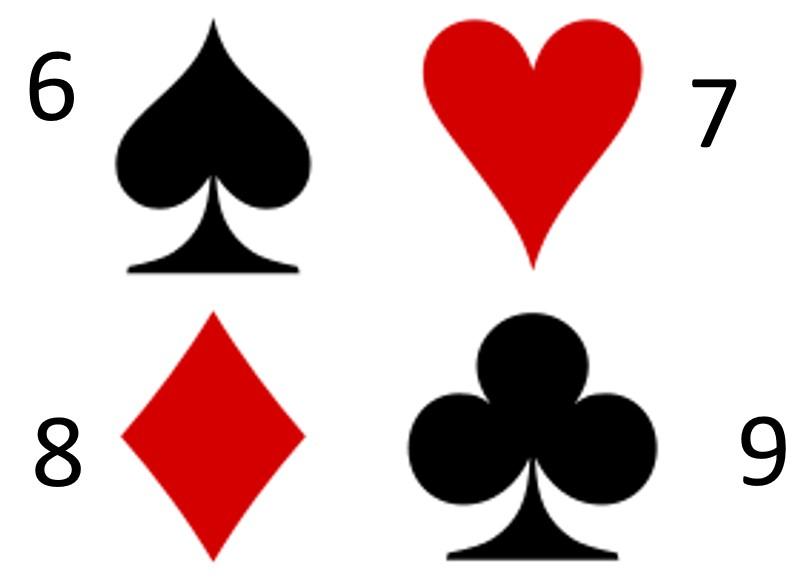
\includegraphics[width=0.2\linewidth]{figurenAuteur/kaartkleuren.jpg}
\end{center}
\end{figure}
Hiermee kun je als goochelaar zeggen welke kaart het was.

\tussentitel{De verklaring; het bewijs dat de truc werkt}

\begin{werktekstoef}
\item{Noem de getalwaarde van de kaart $n$ en het getal van de kleur $5+k$ (dus: $k$ is 1 als het een schoppen kaart is, 2 als het harten is enz.). Maak de berekening uit de instructie met deze variabele getallen.}

\emph{Het getal optellen met het volgende getal geeft $n+(n+1)$. Vereenvoudigen geeft: $n+(n+1)=n+n+1=2n+1$. Dit maal 5 geeft: $(2n+1)\cdot 5=10n+5$. Hierbij wordt de kleur bijgeteld: $10n+5+(5+k)=10n+5+5+k=10n+10+k=10(n+1)+k$.}

\item{Welke kaart werd getrokken als het eindresultaat 34 is? Of 122?}

\emph{$34=10\cdot3+4$. Dus $n+1=3$ en $k=4$. Dus $n=2$ en $5+k=9$. De kaart was klaveren 2. Analoog voor 122: harten boer.
}

\item{Formuleer in het algemeen het geheime recept dat de goochelaar toepast om vertrekkend van het resultaat van de berekening te weten welke kaart het is.}

\emph{Als het cijfer van de eenheden een 1 is, weet je dat het schoppen is, een 2 is harten, een 3 is ruiten en een 4 is klaver. Om de getalwaarde van de kaart te kennen, trek je 1 af van het aantal tientallen.}
\end{werktekstoef}
\eindewerktekst

\\Ook de tweede truc is niet moeilijk. Deze truc was ook vermeld in Uitwiskeling 33/1, p. 26.
\vspace{1cm}

\beginwerktekst{Vliegensvlug optellen}

\tussentitel{De goocheltruc}

De goochelaar vraagt aan iemand van het publiek om twee opeenvolgende getallen onder elkaar te schrijven. Daaronder: de som van die twee getallen. Daaronder: de som van de laatste twee getallen. Dit moet hij herhalen tot er juist zes getallen onder elkaar staan. De goochelaar kan vliegensvlug de som van deze zes getallen opschrijven.

\tussentitel{Voorbeeld}
\begin{center}
87\\
88\\
175\\
263\\
438\\
701   
\end{center}

De som is 1752. Dit is het derde getal waar een 2 achter gezet is.

\tussentitel{Bewijs dat de truc altijd werkt}

\begin{werktekstoef}
\item {Noem het eerste getal $x$. Bepaal voor dit variabel getal de zes getallen en hun som.}

\emph{De getallen zijn}
$$x$$
$$x+1$$
$$x+x+1=2x+1$$
$$x+1+2x+1=3x+2$$
$$2x+1+3x+2=5x+3$$
$$3x+2+5x+3=8x+5.$$
\emph{Hun som is} $$x+x+1+2x+1+3x+2+5x+3+8x+5=20x+12.$$

\item{Laat zien dat die som inderdaad het derde getal is waar een 2 achter gezet is.}

\emph{Er geldt:}
$$20x+12=20x+10+2=10(2x+1)+2.$$
\end{werktekstoef}
\eindewerktekst

\begin{multicols}{2}

De volgende goocheltruc is een klassieker die je in veel boeken terugvindt. Het verklaren ervan is waarschijnlijk te moeilijk voor de modale leerling. Maar soms heb je ook een paar niet-modale leerlingen...

\end{multicols}

\beginwerktekst{Het wondergetal}

\tussentitel{De goocheltruc}

Laat iemand uit het publiek een willekeurig getal van drie verschillende cijfers bedenken en opschrijven, zodat jij het niet kunt zien. Iemand anders moet dit getal omdraaien en weer iemand anders moet het kleinste van het grootste getal aftrekken. Laat dit laatste getal weer omdraaien en deze laatste twee getallen met elkaar optellen. Jij hebt nog altijd niets gezien. Doe alsof je gedachten leest en onthul het eindresultaat: 1089.

\tussentitel{Voorbeeld}
\begin{center}
782\\
$-$287\:\:\,\\
495\\
\underline{+594}\:\:\,\\
1089
\end{center}
\tussentitel{Bewijs dat de truc altijd werkt}
Het gekozen getal kun je schrijven als $100a+10b+c$. Bijvoorbeeld als het getal 349 is, dan is $a=3, b=4$ en $c=9$.
\begin{werktekstoef}
\item{Pas de eerste berekeningen (het omdraaien en het aftrekken) toe op het ‘algemene’ getal $100a+10b+c$. Bewijs dat je een veelvoud van 99 uitkomt.}

\emph{Het getal is:} 		$100a+10b+c$.

\emph{Omgedraaid:}	$100c+10b+a$.

\emph{Verschil:}		$100a+10b+c-(100c+10b+a)=100(a-c)+(c-a)=100(a-c)-(a-c)=99(a-c)$.
\item{Dit zijn alle 99-vouden van twee of drie cijfers: $99, 198, 297, 396, 495, 594, 693, 792, 891, 990$. Wat is er speciaal aan de cijfers van een 99-voud?}

\emph{Het cijfer van de tientallen is altijd 9. De som van de cijfers van de eenheden en de honderdtallen is ook 9.}

\item{Steun op deze eigenschap van 99-vouden om te bewijzen dat de som van een 99-voud en zijn ‘omgedraaide’ altijd 1089 is.}

\emph{Omdat er maar tien gevallen zijn, zou een mogelijk bewijs kunnen zijn: alle gevallen narekenen. Dit is niet slecht. Dit is wat we in vraag 2 deden om de eigenschap van de cijfers te bewijzen van \emph{alle} $99$-vouden. Nog leuker vanuit wiskundig standpunt is om het hier algemener aan te pakken.}

\emph{Steunend op de vastgestelde eigenschap is het 99-voud van de vorm $100d+10\cdot 9+e$ met $d+e=9$. Het omgedraaide getal is $100e+10\cdot 9+d$. Optellen geeft:
$100d+10\cdot 9+e+100e+10\cdot 9+d=100(d+e)+10\cdot 18+e+d=100\cdot 9+10\cdot 18+9=900+180+9=1089$.}

\item{Waarom is de goocheltruc hiermee aangetoond?}

\emph{Het verschil van het gekozen getal en zijn omgedraaide is een 99-voud (vraag 1). In 3 hebben we bewezen dat de som van dit verschil en zijn ‘omgedraaide’ altijd gelijk is aan $1089$.}
\end{werktekstoef}
\eindewerktekst

\begin{multicols}{2}
Naast het werken met een variabele als willekeurig getal en het toepassen op formules van rekenregels die gelden voor getallen, komt in de vorige werktekst nog iets aan bod: de betekenis van de cijfers in een getal (in het tiendelig talstelsel): het getal 346 is $3\cdot 100+4\cdot 10+6$. In het wondergetal werd op die manier een ‘willekeurig’ natuurlijk getal van drie cijfers geschreven als $a\cdot 100+b\cdot 10+c$ (waarbij $a$,$b$ en $c$ de cijfers zijn). Ook deelbaarheid komt aan bod (de 99-vouden).

\subsection{Deelbaarheid}

Deelbaarheid, even, oneven, deelbaarheidskenmerken: deze begrippen vormen een prima context voor kleine bewijsjes, door te rekenen met letters maar soms ook door te werken met een generiek voorbeeld. Strikt genomen is het geen bewijs als je op een concreet voorbeeld werkt, maar je kunt het idee van een bewijs er wel mee tonen. Dat bewijs-idee kun je vaak ook visueel maken, door de getallen voor te stellen als patronen. Het is belangrijk dat je met de leerlingen vragen over bewijzen bespreekt: wat is een bewijs, waarom volstaat het uitrekenen op voorbeelden niet, waarom ben je zeker dat je bewijs-idee altijd werkt...?

Dat de som van drie opeenvolgende getallen altijd een drievoud is, kun je met letters bewijzen: noem de getallen $n$, $n+1$ en $n+2$. De som is $n+n+1+n+2=3n+3=3(n+1)$. Dit bewijsidee kun je met een voorbeeld tonen. Neem bv. $13+14+15$. Als je de som gewoon uitrekent en vaststelt dat het een drievoud is, dan `bewijs' je nog niets. Maar door te schrijven $13+13+1+13+2=3\cdot 13+3=3\cdot (13+1)=3\cdot 14$ overtuig je wel dat je dit voor elk getal kunt doen, niet alleen voor 13. Je kunt het ook visualiseren: onder elkaar rijtjes van 13, 14 en 15 punten `herschikken' tot een rechthoek van 3 rijen van 14 (door het verste puntje van die 15 te verplaatsen achter de rij van 13):

o  o  o  o  o  o  o  o  o  o  o  o  o\\
o  o  o  o  o  o  o  o  o  o  o  o  o  o\\
o  o  o  o  o  o  o  o  o  o  o  o  o  o  o

Om bv. het kenmerk van deelbaarheid door $9$ te bewijzen, kun je werken met een generiek voorbeeld:  
\begin{center}
een (natuurlijk) getal is deelbaar door $9$\\ $\Leftrightarrow$ de som van de cijfers is deelbaar door $9$
\end{center}

Neem bv. het getal 576. Er geldt:
\begin{align}
576&=5\cdot 100+7\cdot 10+6 \nonumber\\
&=5\cdot(99+1)+7\cdot(9+1)+6 \nonumber\\
&=5\cdot99+5+7\cdot9+7+6 \nonumber\\
&=5\cdot99+7\cdot9+5+7+6 \nonumber\\
&=\text{een negenvoud}+(5+7+6)  \nonumber
\end{align}

Zo’n voorbeeld is wat de redenering betreft `algemeen'; werken met een willekeurig getal van drie cijfers zou hetzelfde zijn behalve dat 5, 6 en 7 vervangen zouden zijn door letters $a, b$ en $c$. Om heel algemeen te zijn, zou ook het aantal cijfers willekeurig moeten zijn en zou men moeten werken met $a_n 10^n+a_{n-1}10^{n-1}+...+a_0$, maar dit zou voor het begrijpen van het `waarom’ hier eigenlijk geen meerwaarde hebben

Voor getallen kleiner dan 100 kunnen we het ook visueel voorstellen. Om in het getallenrooster hieronder van het ene negenvoud naar het volgende te springen, tel je één tiental bij (ga je één stap naar beneden) en trek je één eenheid af (ga je één stap naar links). Op die manier blijft de som van het aantal cijfers ongewijzigd. Omdat bij 9 de som van de cijfers uiteraard een negenvoud is, is dit ook zo voor de andere negenvouden.

\begin{footnotesize}

\begin{tabular}{r r r r r r r r r r r}
1  &2  &3  &4  &5  &6  &7  &8  &\textbf{9}  &10\\
11 &12 &13 &14 &15 &16 &17 &\textbf{18} &19 &20\\
21 &22 &23 &24 &25 &26 &\textbf{27} &28 &29 &30\\
31 &32 &33 &34 &35 &\textbf{36} &37 &38 &39 &40\\
41 &42 &43 &44 &\textbf{45} &46 &47 &48 &49 &50\\
...
\end{tabular}
\end{footnotesize}

Een suggestie van Numberphile (Padilla, s.d.) is om ook kenmerken van deelbaarheid voor te stellen als goocheltoeren. Je geeft bv. aan een deelnemer een pakje van 9 kaarten genummerd 1(=aas), 2, 3, ...9. De deelnemer moet die allemaal op tafel leggen in een zelfgekozen volgorde en zo een getal van 9 cijfers maken. Je beweert: ``Ik voel dat je een negenvoud hebt gemaakt.'' De klas controleert met een rekenmachine. Dan mag de deelnemer de volgorde veranderen en een kaart wegnemen (of toevoegen uit de kaarten van een andere kleur). Jij neemt ook een kaart weg (of voegt ook een kaart toe). Opnieuw een negenvoud.
Hoe werkt dit? De som van de cijfers, ``1+2+3+4+5+6+7+8+9=45'', is een negenvoud. Daarom is het getal, wat de volgorde ook weze, een negenvoud. De som van de cijfers verandert niet als je de volgorde verandert. Als de deelnemer bv. de 6 heeft weggenomen, neem jij de 3 weg. Of als de deelnemer bv. een 2 toevoegt, voeg jij een 7 toe. Je zorgt ervoor dat de som van de cijfers een negenvoud blijft.

In feite kun je heel veel eigenschappen van getallen presenteren als goocheltrucs en ze hiermee (nog) aantrekkelijker maken voor de leerlingen.


\subsection{Redeneren met patronen en formules}

In Krysinska (2018) en Guissard \& Wettendorff (2018a, 2018b) vond ik onlangs mooie activiteiten waarin leerlingen zoeken naar een patroon in een rij figuurtjes en dit patroon met een formule uitdrukken.

Dit aspect komt ook voor in de huidige eindtermen en leerplannen, onder meer onder impuls van Uitwiskeling. Zie onze loep ‘Getallen en meetkunde in de eerste graad’ (Eggermont, Roelens, 1995), die verschenen is kort voor het leerplan van de eerste graad van 1997. Zie ook de loep ‘Patronen leren herkennen’ (Op de Beeck, R., Willems, J., 2010). Deze loepen zijn  nog steeds het lezen waard.

De eerste drie werkteksten hieronder zijn sterk geïnspireerd op Krysinska (2018). De vierde, over vierkante en rechthoekige matten, op Guissard \& Wettendroff (2018).
\end{multicols}
\newpage
\beginwerktekst{Een huizenrij met lucifers}

Hieronder zie je hoe een huizenrij gemaakt wordt met lucifers. Enkel de eerste drie stappen zijn getoond.

\begin{figure}[H]
\begin{center}
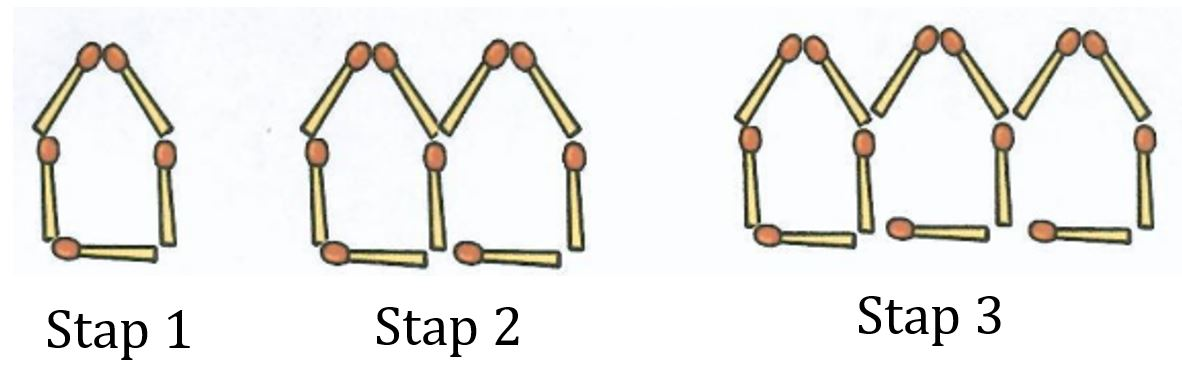
\includegraphics[width=0.40\linewidth]{figurenAuteur/luciferhuisjes2}
\end{center}
\end{figure}
\begin{werktekstoef}
\item{Maak een tabel met het aantal lucifers voor een rij met 1, 2, ..., 5 huisjes.}
\item{Zoek een patroon in die tabel. Verklaar dit patroon door de manier waarop de huisjes gemaakt zijn.}
\item{Hoeveel lucifers heb je nodig voor een rij van 10 huisjes?}
\item{Maak een formule voor het aantal lucifers in een rij met $n$ huisjes.}
\item{Vergelijk je formule met de formule van andere groepjes. Misschien heb je een andere redenering gevolgd maar komt het toch op hetzelfde neer… Bewijs dat het op hetzelfde neerkomt.}

\emph{Bv. de ene groep heeft geredeneerd: het eerste huisje is gemaakt met 5 lucifers en telkens worden 4 lucifers toegevoegd. Dit leidt tot de formule: aantal lucifers $=5+(n-1)\cdot 4$. Een andere groep kan gedacht hebben: 5 lucifers per huisje min het aantal gemeenschappelijke lucifers. Dit geeft voor het aantal lucifers $=n\cdot 5-(n-1)$. Nog een andere groep heeft in de tabel gezien dat het aantal lucifers in de $n$-de stap gelijk is aan $4n+1$. Met rekenregels kan aangetoond worden dat die formules op hetzelfde neerkomen.}

\item{Je beschikt over 100 lucifers. Na welke stap zijn er te weinig over om nog een nieuw huisje te kunnen toevoegen?}

\emph{De leerlingen moeten niet enkel de vergelijking $4n+1=100$ oplossen ($n=\frac{99}{4}$) maar ook naar onder afronden. Na de 24ste stap dus.}

\end{werktekstoef}
\eindewerktekst

\beginwerktekst{Een groeiende rechthoek}

Hieronder zie je een rechthoek gemaakt met M\&M’s. De rechthoek wordt stap voor stap groter.

\begin{figure}[H]
\begin{center}
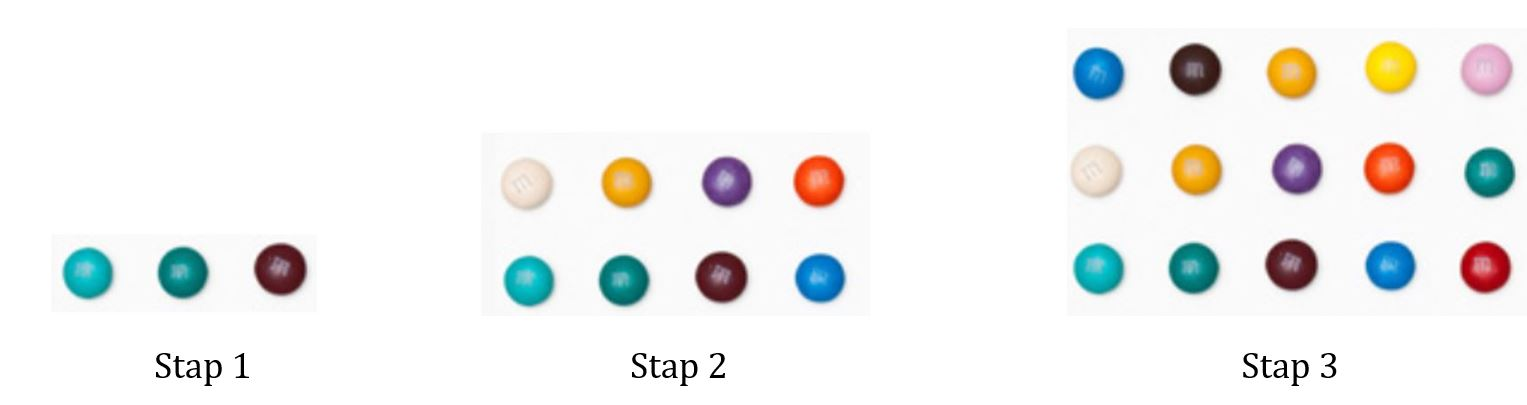
\includegraphics[width=0.7\linewidth]{figurenAuteur/menmrechthoeken2.JPG}
\end{center}
\end{figure}
\begin{werktekstoef}
\item{Maak een tabel met het aantal M\&M’s na stap 1, stap 2, … stap 5.}

\item{Zoek een patroon. Maak een formule voor het aantal M\&M’s na stap $n$.}

\item{Vergelijk je formule met die van de andere groepjes.}

\item{Hoever geraak je met drie zakjes van elk 34 M\&M’s?}
\end{werktekstoef}
\eindewerktekst
\newpage
\beginwerktekst{De takken van de boom}

Een boom heeft eerst twee takken en vanaf dan vertakt elke tak in drie.

\begin{figure}[H]
\begin{center}
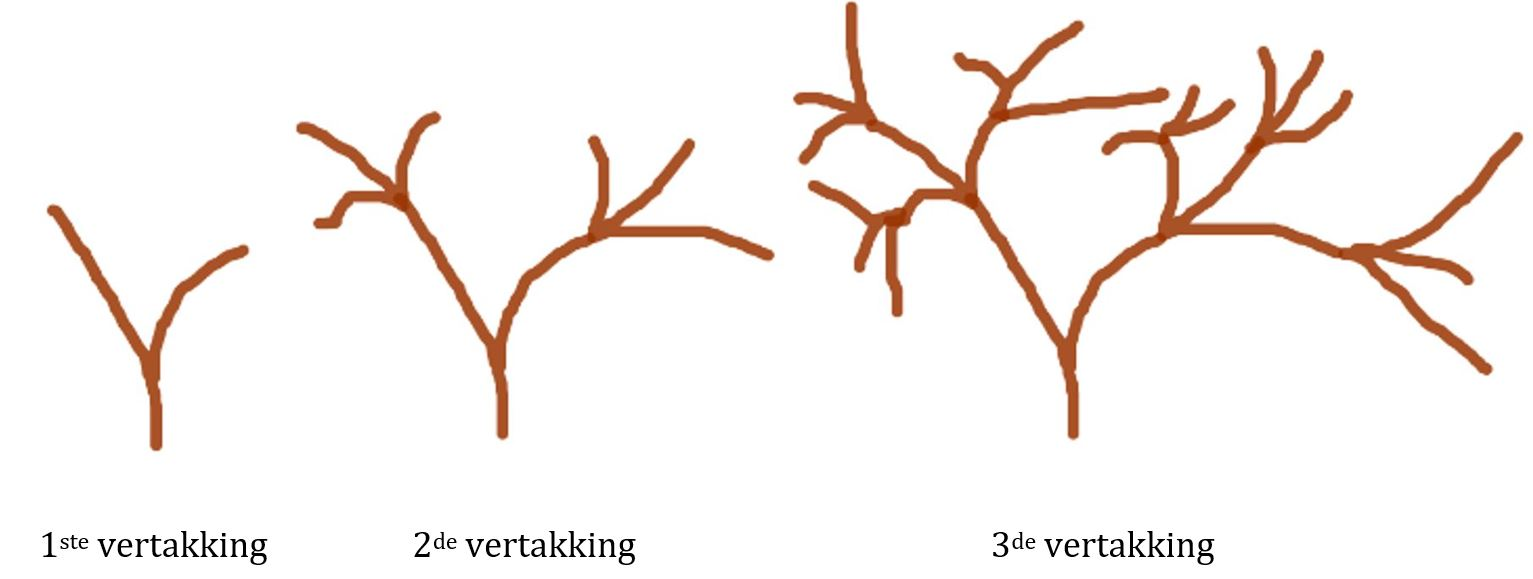
\includegraphics[width=0.8\linewidth]{figurenAuteur/groeiendeboom2.JPG}
\end{center}
\end{figure}

\begin{werktekstoef}
\item{Maak een tabel met aantal nieuwe takjes bij de 1ste, 2de , … 5de vertakking.}
\item{Zoek een patroon. Maak een formule voor het aantal nieuwe takjes bij de $n$-de vertakking.}
\item{Vergelijk je formule met die van de andere groepjes.}
\item{Hoeveel nieuwe takjes ontstaan er bij de 10de vertakking? En hoeveel takken zijn er dan in totaal (de stam niet meegerekend)?}

\end{werktekstoef}
\eindewerktekst

\begin{center}
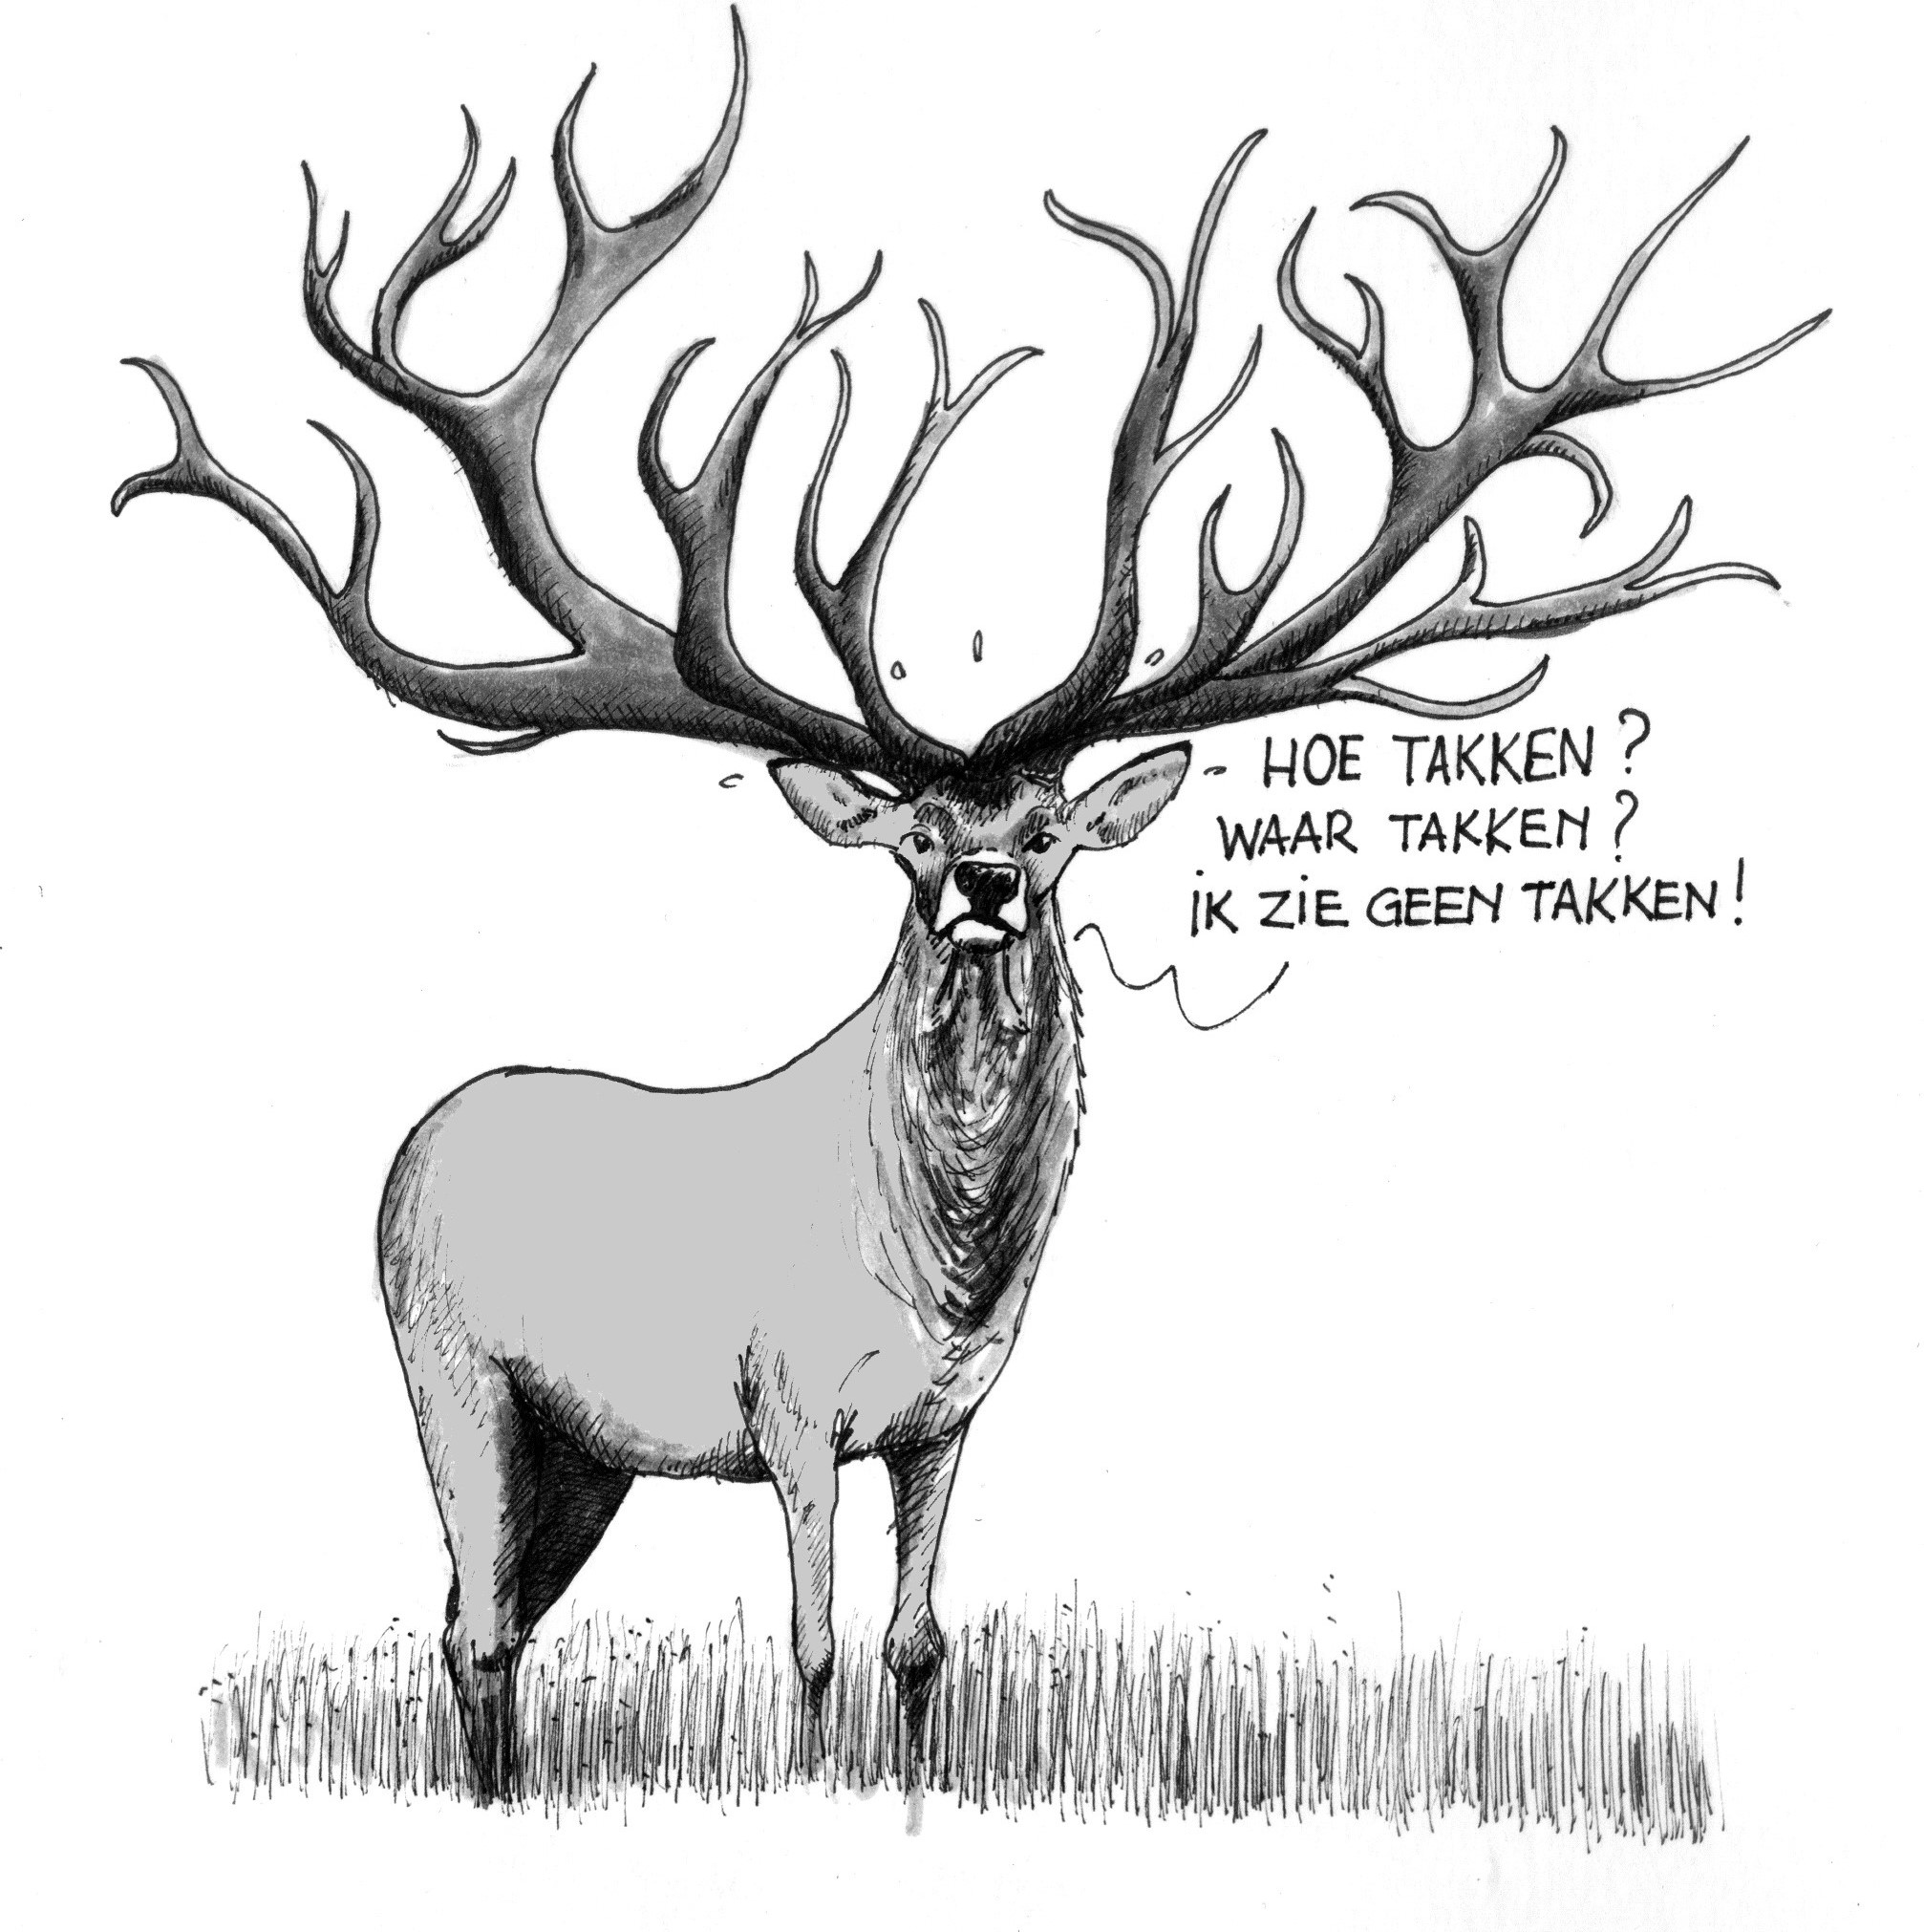
\includegraphics[width=0.65\linewidth]{tekeningenKurt/takken.jpg}
\end{center}
\begin{multicols}{2}

Zoals vaak presenteren we de volgende activiteit met vragen en antwoorden, maar dat wil niet zeggen dat de leerlingen alles zelfstandig of in groepjes moeten afwerken. Het best lijkt ons een afwisseling tussen korte werkmomenten in duo’s of groepjes met klassikale besprekingen. Je kunt je ook beperken tot enkel de vierkante of enkel de rechthoekige matten. Van de rechthoekige matten zijn er twee soorten. Eventueel kun je die verdelen: de helft van de klas doet de eerste soort en de andere helft de tweede.
\end{multicols}

\beginwerktekst{Matten van vierkante tegels}

Er komt een nieuwe soort vierkante matten op de markt. Ze bestaan uit gelijke vierkante tegels. De buitenste tegels zijn gekleurd en de binnenste zijn wit, zoals op de figuur. De kleinste heeft maar één witte tegel in het midden en de grootste heeft acht witte tegels per zijde van de binnenkant. Hieronder zie je de mat met twee witte tegels per binnenzijde.

\begin{figure}[H]
\begin{center}
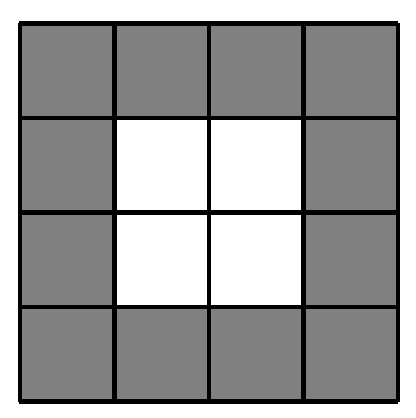
\includegraphics[width=0.15\linewidth]{figurenAuteur/vierkantemat}
\end{center}
\end{figure}

\begin{werktekstoef}
\item{Is het mogelijk om zo’n vierkante mat te hebben met evenveel witte als gekleurde tegels? Leg uit hoe je te werk gaat.}

\emph{Een eerste methode die de leerlingen kunnen toepassen is: al deze matten tekenen en tellen. Ze stellen vast dat er geen enkele bij is met evenveel witte als gekleurde tegels.}

\emph{Een tweede methode, die je kunt voorstellen aan leerlingen die niet weten hoe te beginnen, is het maken van een tabel.}
\emph{
\begin{center}
  \begin{tabular}{ | c | c | c | }
    \hline
     Aantal witte tegels per binnenzijde & Aantal witte tegels & Aantal gekleurde tegels \\ \hline
    1 & 1 & 8 \\ \hline
    2 & 4 & 12 \\ \hline
    3 & 9 & 16 \\ \hline
    4 & 16 & 20 \\ \hline
    5 & 25 & 24 \\ \hline
    6 & 36 & 28 \\ \hline
    7 & 49 & 32 \\ \hline
    8 & 64 & 36 \\ \hline
  \end{tabular}
\end{center}}
\emph{Ze stellen vast dat het aantal witte tegels nooit gelijk is aan het aantal gekleurde. Als de matten groter worden, komen deze aantallen eerst dichter bij elkaar en daarna gaan ze weer verder uit elkaar. Dit doet vermoeden dat ook bij grotere matten, buiten de tabel, de aantallen niet gelijk zullen zijn. 
Voor de volgende vraag hebben alle leerlingen deze tabel nodig (ook als zij die niet gebruikt hebben bij het zoeken van het antwoord op vraag 1).
}

\end{werktekstoef}

De tabel bevat heel wat regelmaat.

\begin{werktekstoef}
\setcounter{enumi}{1}

\item{Hoe ga je van kolom 1 naar kolom 2? En hoe ga je van kolom 1 naar kolom 3. Je kunt naar de getallen kijken, maar je kunt ook een tekening van een mat gebruiken.}

\emph{De tweede kolom bevat de kwadraten van de getallen van de eerste kolom. Hoe ga je van de eerste naar de derde kolom? De leerlingen ontdekken, met de getallen of visueel aan de hand van de matten, dat je met 4 moet vermenigvuldigen (vier zijden) en nog 4 bijtellen (de vier ‘hoekjes’). Andere leerlingen zeggen: 1 bijtellen en dan met vier vermenigvuldigen. Ook dat is visueel te verklaren.}

\begin{figure}[H]
\begin{center}
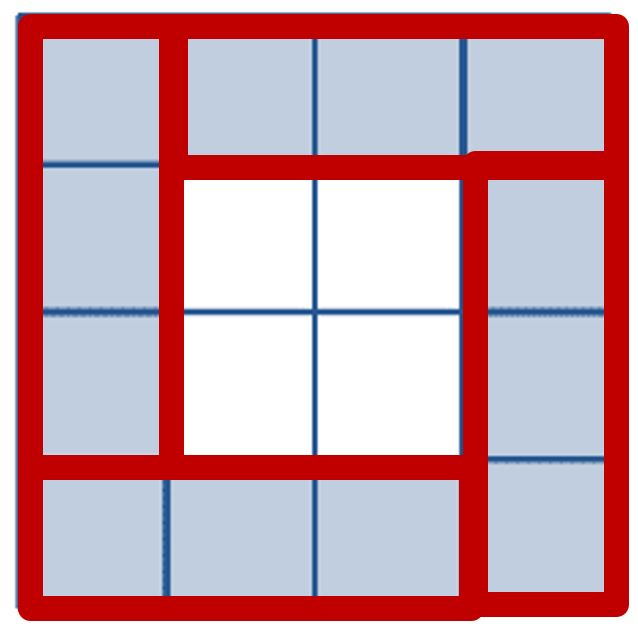
\includegraphics[width=0.15\linewidth]{figurenAuteur/vierkantemat2}
\end{center}
\end{figure}

\emph{Wanneer de leerlingen dan (samen met de leerkracht) het verband tussen de eerste en de derde kolom in een formule uitdrukken, geeft dat twee mogelijkheden die op hetzelfde neerkomen. Noem $w$ het aantal witte tegels per zijde van de binnenkant, dan is het aantal gekleurde tegels $g$ te schrijven als $g=4w+4$, maar ook als $g=4(w+1)$. Dit levert de gelijkheid $4w+4=4(w+1)$ op, een (her)ontdekking van de distributiviteit van de vermenigvuldiging ten opzichte van de optelling. Nog anderen geven een uitleg die neerkomt op $g=2w+2(w+2)$ of zelfs $g=(w+2)^2-w^2$. Beiden zijn ook visueel te ontdekken of te verklaren.}

\begin{figure}[H]
\begin{center}
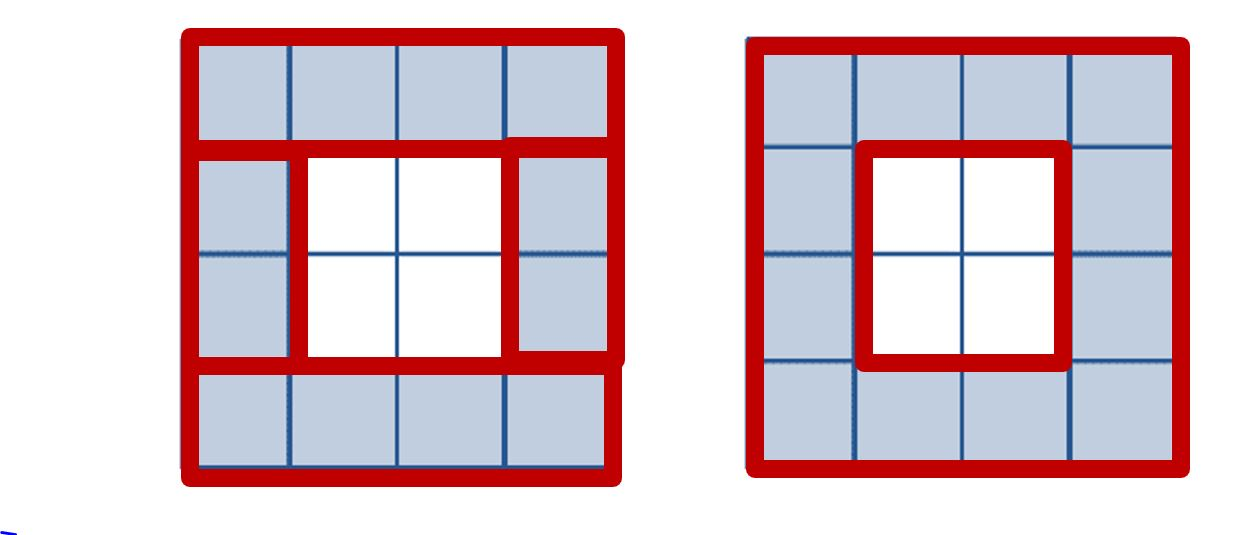
\includegraphics[width=0.41\linewidth]{figurenAuteur/vierkantemat3}
\end{center}
\end{figure}

\emph{Ook al gebruik je voor het visualiseren van de verklaring een voorbeeld (bv. een mat met twee tegels aan elke binnenzijde zoals hierboven), het is duidelijk dat je dit analoog kunt doen voor andere vierkante matten. Ook al is het strikt genomen geen bewijs ``voor elke $w$'' (zoals een bewijs door volledige inductie), toch beschouwen we dit als een overtuigend (preformeel) bewijs.}

\item{Zie je ook verbanden binnen één zelfde kolom?}

\emph{In de derde kolom is elk getal gelijk aan het getal erboven vermeerderd met vier. In de tweede kolom worden opeenvolgende oneven getallen bijgeteld: plus 3, plus 5, plus 7… Dit kan, met wat hulp van de leraar, ook visueel worden geïllustreerd/bewezen.}

\end{werktekstoef}
\begin{figure}[H]
\begin{center}
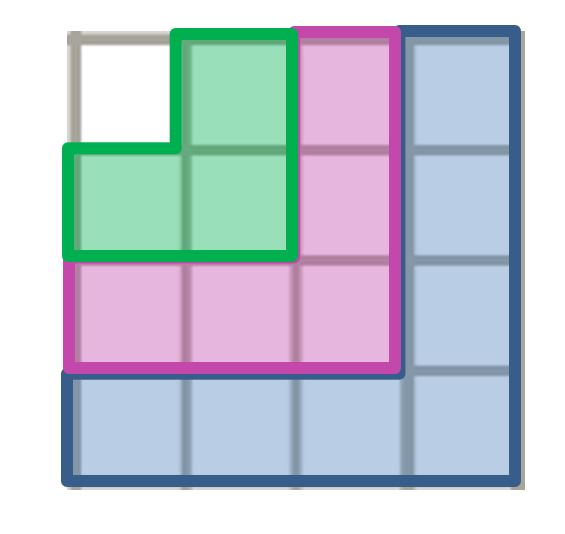
\includegraphics[width=0.20\linewidth]{figurenAuteur/vierkantemat4}
\end{center}
\end{figure}

Er komen twee nieuwe soorten matten op de markt. Ze bestaan ook uit gelijke vierkante tegels: witte in het midden en daarrond een gekleurde boord van tegels. Maar de witte tegels binnenin hoeven geen vierkant meer te vormen. Bij de eerste soort vormen de witte tegels een rechthoek met drie tegels op één van de zijden. Bij de tweede soort vormen de witte tegels een rechthoek met vijf tegels op één van de zijden. Het aantal tegels op de andere zijde kan telkens variëren.

\begin{figure}[H]
\begin{center}
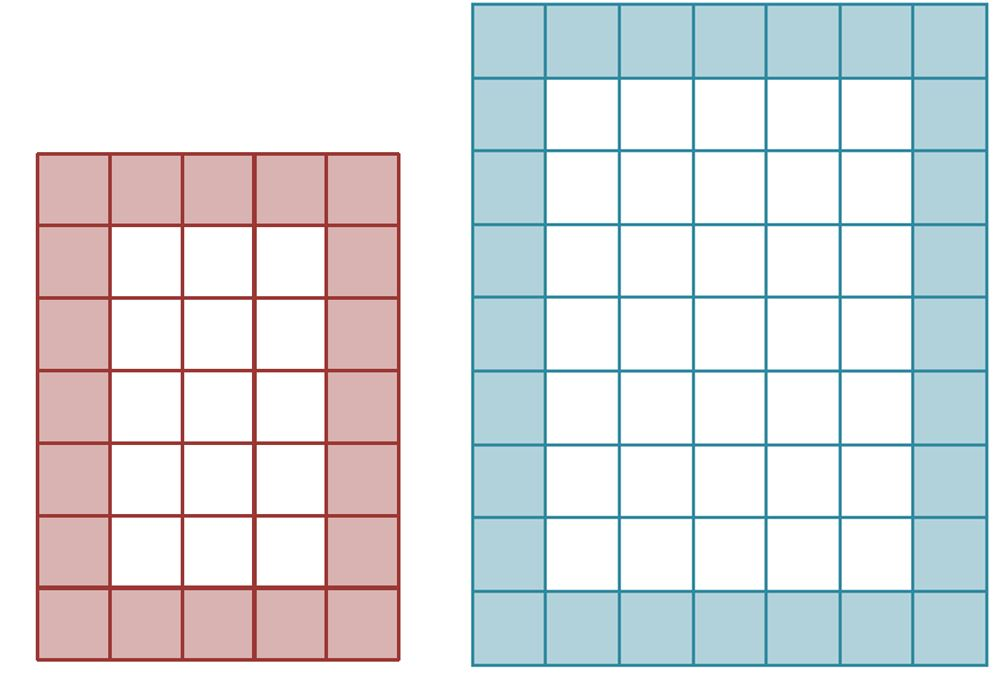
\includegraphics[width=0.5\linewidth]{figurenAuteur/rechthoekigematten}
\end{center}
\end{figure}

\begin{werktekstoef}
\setcounter{enumi}{3}  
\item{Kunnen er bij deze soorten matten evenveel witte als gekleurde tegels zijn?}

\emph{De leerlingen kunnen opnieuw voor beide situaties een tabel maken: de eerste kolom is het aantal rijen van witte tegels in het midden, de tweede kolom het aantal witte tegels en de derde kolom het aantal gekleurde tegels. (We nemen deze tabel hier niet op.) Leerlingen zien dat er bij de eerste soort wel een oplossing is en bij de tweede niet. Maar: er is geen grens gesteld aan het aantal rijen. Zijn we zeker dat er in het eerste geval maar één oplossing is en dat er bij de tweede soort niet buiten de tabel nog een oplossing kan zijn?}\\

\emph{De leerlingen kunnen weer, met de tabel of met een tekening van de matten, formules maken voor het aantal witte en gekleurde tegels. Noem $r$ het aantal rijen van witte tegels.}\\

\emph{Bij de eerste soort: $w=3r$ (voorgesteld door 
$\circ$); $g=2r+10$ (voorgesteld door $\diamond$).}\\

\emph{Bij de tweede soort: $w=5r$ (voorgesteld door $\circ$), $g=2r+14$ (voorgesteld door $\diamond$).}\\

\emph{De punten $(r,\: w)$ liggen op één rechte. Ook de punten $(r,\: g)$ liggen op één rechte. In het eerste geval snijden deze rechten elkaar in het punt $(10,\: 30)$: bij de mat met 10 witte rijen heb je evenveel witte als gekleurde tegels, namelijk 30. In het tweede geval liggen die punten ook telkens op een rechte, maar deze rechten snijden elkaar niet in een roosterpunt met gehele coördinaten. Dit overtuigt dat er in het eerste geval juist één oplossing is en in het tweede geval geen oplossing.}

\begin{figure}[H]
\begin{center}
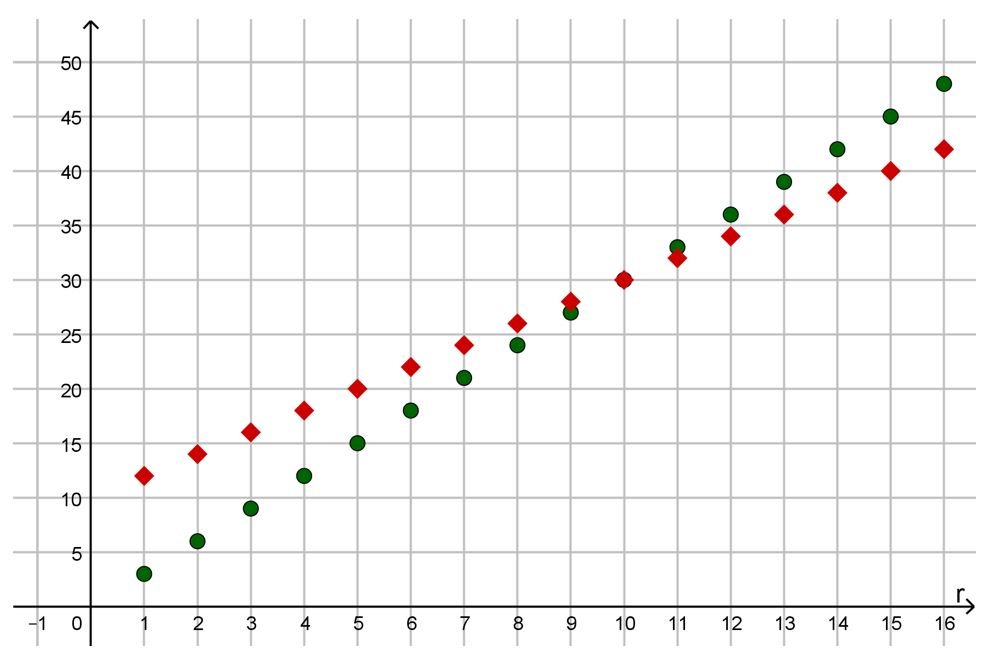
\includegraphics[width=0.66\linewidth]{figurenAuteur/rechthoekigemattengrafiek1}\\
\emph {Grafiek: eerste soort matten}
\end{center}
\end{figure}

\begin{figure}[H]
\begin{center}
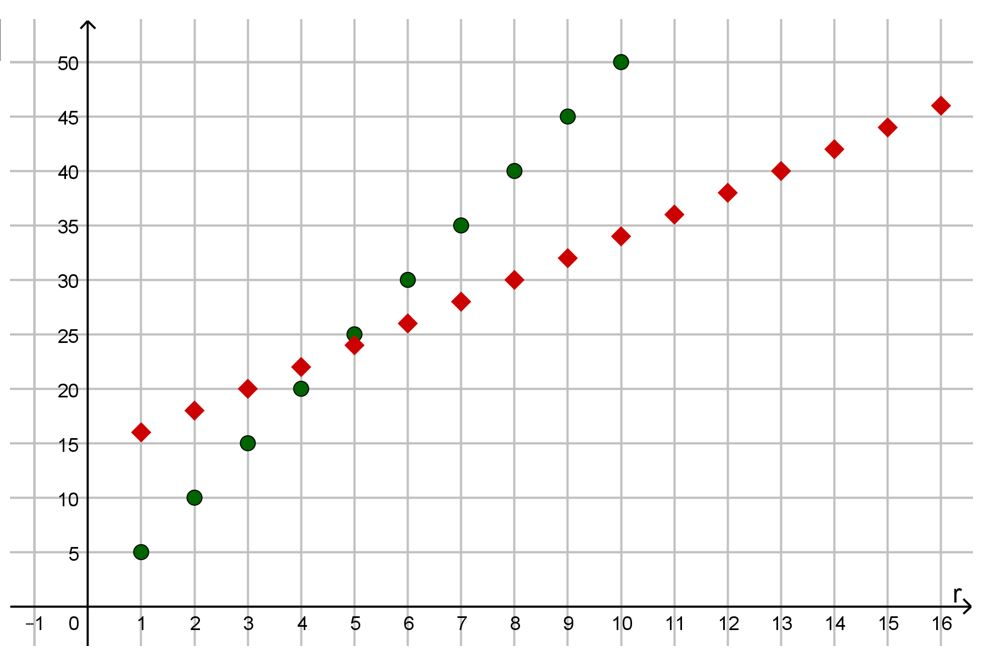
\includegraphics[width=0.6\linewidth]{figurenAuteur/rechthoekigemattengrafiek2}\\
\emph {Grafiek: tweede soort matten}
\end{center}
\end{figure}




\emph{Je kunt het probleem in plaats van grafisch, ook algebraïsch oplossen. Uitdrukken dat het aantal witte tegels $w$ gelijk is aan het aantal gekleurde tegels $g$, levert een vergelijking op in $r$.}

\emph{Bij de eerste soort: $3r=2r+10$ (oplossing: $r=10$). Bij de tweede soort: $5r=2r+14$ (oplossing: $r=\frac{14}{3}$, dus geen oplossing want het aantal rijen moet geheel zijn).}

\emph{Merk op: als je ook bij het probleem van de vierkante matten een grafiek zou maken, dan zou je een parabool met een rechte moeten snijden. Uiteraard kunnen de leerlingen van de eerste graad dit niet met een vergelijking oplossen.}

\end{werktekstoef}
\eindewerktekst

\begin{multicols} {2}

\section{Bewijzen met hoeken}
\subsection{Hoeken en evenwijdigheid}

We willen hier het voorbeeld van ‘verwisselende binnenhoeken’ (in Nederland: Z-hoeken) aangrijpen om het te hebben over een stelling en haar omgekeerde en over een bewijsje uit het ongerijmde. We gaan ervan uit dat de leerlingen al transformaties en hun eigenschappen gezien hebben. Een voordeel van het gebruik van transformaties is dat de eigenschappen van deze transformaties dan gebruikt worden. Het heeft weinig zin deze eigenschappen vast te stellen en te formuleren als er daarna niets meer mee gebeurt. Er is een tijd geweest dat de congruentiekenmerken in het secundair onderwijs ‘bewezen’ werden aan de hand van transformaties. Dit paste in een meer globale deductieve opbouw. Daar pleiten we niet voor. Meer uitleg hierover in onze loep over transformaties (UW14/3). We vermelden hier zowel hoe je het met transformaties kunt doen als zonder.

Bij deze activiteit horen, per duo leerlingen, twee kartonnen hoeken van de grootte van $\hat{A}_1$ en $\hat{A}_2$. De leerlingen kunnen die gebruiken niet alleen om vast te stellen dat hoekgroottes gelijk zijn maar ook om te zien welke transformaties bruikbaar zijn. In vraag 6 vragen we aan de leerlingen om de gelijkheid van overstaande hoeken te bewijzen, zonder dit te sturen via deelvraagjes. Dit wil niet zeggen dat alle leerlingen dit meteen zullen kunnen. Indien nodig helpt de leraar wel met tips zoals “kun je gebruik maken van nevenhoeken?” of “misschien is er een transformatie die hier nuttig is”.

Nog een opmerking over de benamingen: sommige boeken spreken over verwisselende binnen- en buitenhoeken ook wanneer de twee rechten waarbinnen of waarbuiten deze hoeken zich bevinden, niet evenwijdig zijn. In dat geval zegt de eigenschap: ``als die twee rechten evenwijdig zijn, dan zijn de verwisselende binnenhoeken (of buitenhoeken) gelijk''. Wij gebruiken de term verwisselende binnenhoeken enkel wanneer deze twee rechten evenwijdig zijn. De eigenschap luidt dan dat verwisselende binnenhoeken (of buitenhoeken) altijd gelijk zijn. Het is voor de leraar nuttig om bewust te zijn van het bestaan van deze twee versies.

\end{multicols}

\beginwerktekst{Gelijkheid van hoeken bij twee evenwijdige rechten gesneden door een derde rechte}

Om over hoeken bepaalde zaken te kunnen bewijzen (bv. de som van de hoeken in een driehoek), hebben we een verband nodig tussen evenwijdigheid en hoekgrootte.

\tussentitel{Eigenschappen van hoeken bij evenwijdige rechten vaststellen}

Hieronder zijn de rechten $a$ en $b$ evenwijdig. Ze worden gesneden door de rechte $c$. De snijpunten zijn $A$ en $B$.

\begin{figure}[H]
\begin{center}
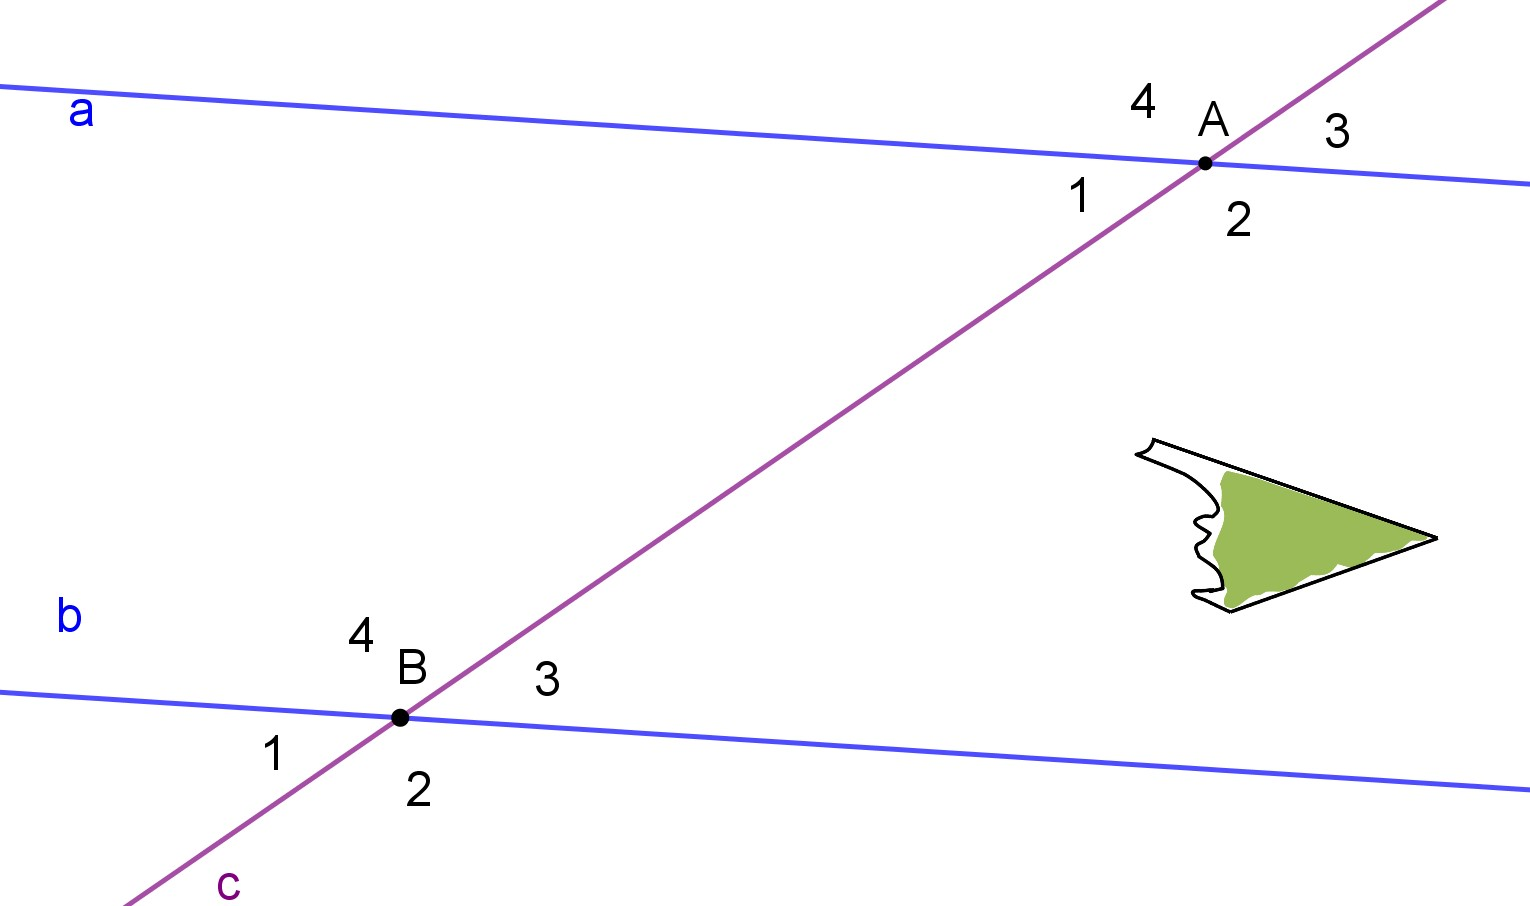
\includegraphics[width=0.5\linewidth]{figurenAuteur/zhoeken1}
\end{center}
\end{figure}

\begin{werktekstoef}
\item Welke hoeken zijn nevenhoeken? Waarom?

\emph{De hoeken $\hat{A}_1$ en $\hat{A}_2$, $\hat{A}_2$ en $\hat{A}_3$, $\hat{A}_3$ en $\hat{A}_4$ ,  $\hat{A}_4$ en $\hat{A}_1$ en ook de hoeken $\hat{B}_1$ en $\hat{B}_2$, $\hat{B}_2$ en $\hat{B}_3$, $\hat{B}_3$ en $\hat{B}_4$, $\hat{B}_4$ en $\hat{B}_1$. Dit zijn telkens nevenhoeken omdat ze één been gemeenschappelijk hebben en omdat hun andere benen telkens één rechte vormen.}

\item Wat weet je over de hoekgroottes van nevenhoeken?

\emph{We weten dat nevenhoeken supplementair zijn: hun som is 180°.}

\end{werktekstoef}

We geven namen aan bepaalde paren van hoeken bij twee evenwijdige rechten en een snijlijn.
\begin{opsomming}
\item{De hoeken $\hat{A}_1$ en $\hat{A}_3$ noemen we \textbf{overstaande hoeken} (in Nederland: X-hoeken).}
\item{De hoeken $\hat{A}_1$ en $\hat{B}_1$ noemen we \textbf{overeenkomstige hoeken} (in Nederland: F-hoeken).}
\item{De hoeken $\hat{A}_1$ en $\hat{B}_3$ noemen we \textbf{verwisselende binnenhoeken} (in Nederland: Z-hoeken).}
\item{De hoeken $\hat{A}_3$ en $\hat{B}_1$ noemen we \textbf{verwisselende buitenhoeken}.}
\end{opsomming}

\begin{werktekstoef}
\setcounter{enumi}{2}  

\item{Verklaar deze benamingen.}

\emph{Bv. voor verwisselende binnenhoeken: deze hoeken liggen ‘binnen’ de evenwijdige rechten en aan ‘wisselende’ kanten van de snijlijn. De Nederlandse benamingen: omdat deze soort hoeken voorkomen in die hoofdletters (als we die letters als meetkundige figuren opvatten).}
\item{Geef van elke soort een ander paar uit dezelfde figuur.}

\emph{Bv. voor verwisselende binnenhoeken: $\hat{A}_2$ en $\hat{B}_4$}

\item{Noteer alle hoeken van de figuur waarvan je vermoedt dat ze gelijk zijn aan $\hat{A}_1$. Je mag dit controleren met één van de kartonnen hoeken. Welke hiervan vormen met $\hat{A}_1$ overstaande, overeenkomstige, ... hoeken? }

\emph{De overstaande hoeken $\hat{A}_1$ en $\hat{A}_3$ zijn gelijk.}

\emph{De overeenkomstige hoeken $\hat{A}_1$ en $\hat{B}_1$ zijn gelijk.}

\emph{De verwisselende binnenhoeken $\hat{A}_1$ en $\hat{B}_3$ zijn gelijk.}

\begin{figure}[H]
\begin{center}
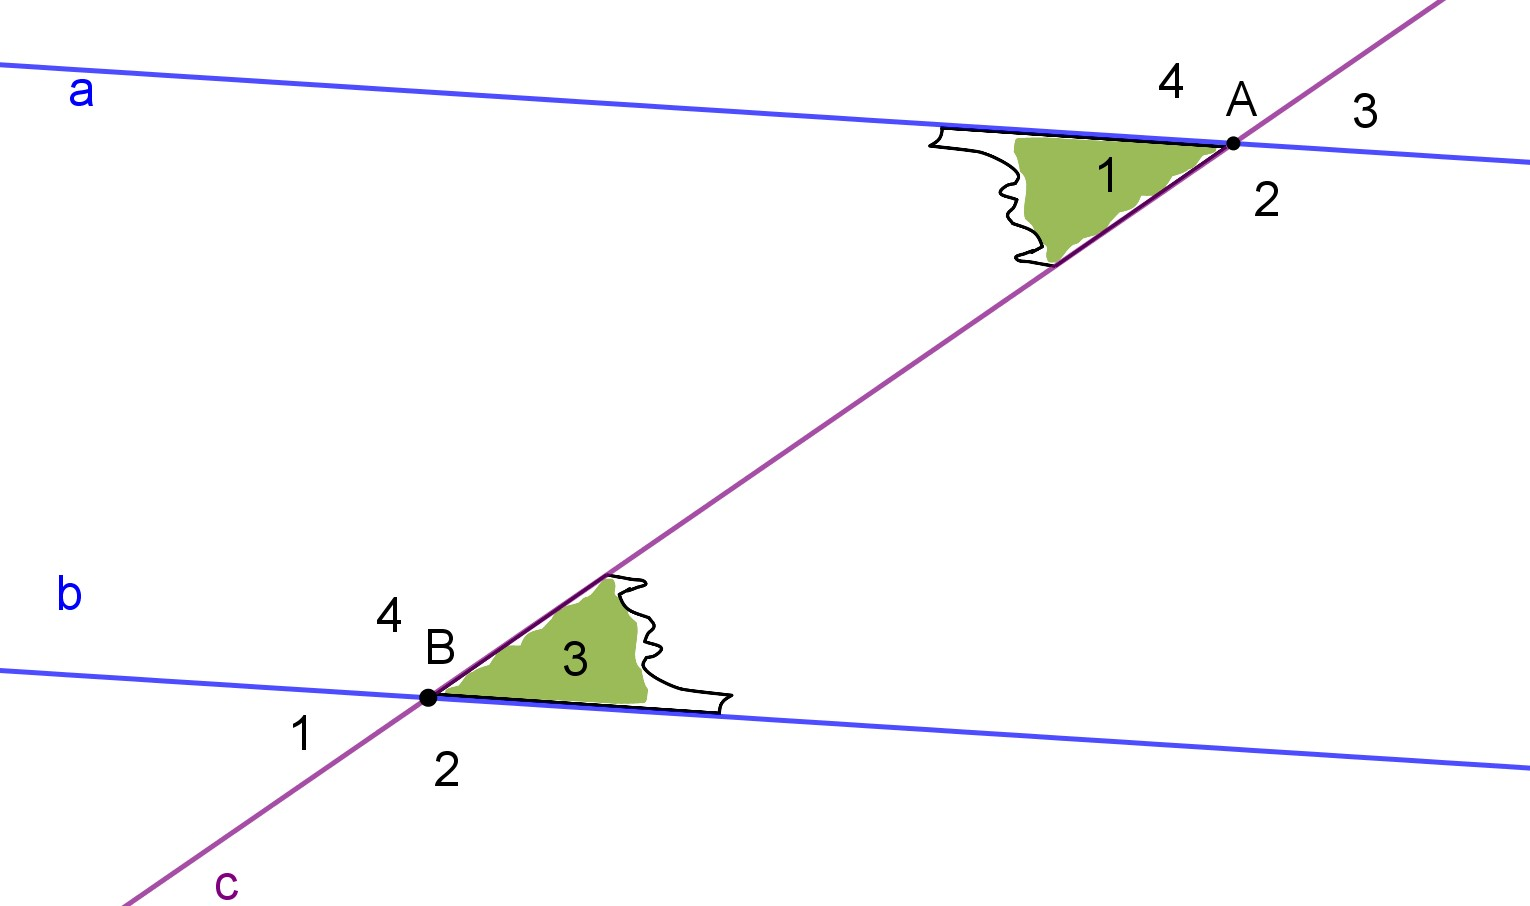
\includegraphics[width=0.5\linewidth]{figurenAuteur/zhoeken2}
\end{center}
\end{figure}

\item{Noteer alle hoeken van de figuur waarvan je vermoedt dat ze gelijk zijn aan $\hat{A}_4$. Welke hiervan vormen met $\hat{A}_4$ overstaande, overeenkomstige, ... hoeken.}

\emph{De overstaande hoeken $\hat{A}_4$ en $\hat{A}_2$ zijn gelijk.}

\emph{De overeenkomstige hoeken $\hat{A}_4$ en $\hat{B}_4$ zijn gelijk.}

\emph{De verwisselende buitenhoeken $\hat{A}_4$ en $\hat{B}_2$ zijn gelijk.}

\end{werktekstoef}

\tussentitel{Deze eigenschappen bewijzen}

\begin{werktekstoef}
\setcounter{enumi}{6}  

\item{Bewijs dat de overstaande hoeken $\hat{A}_1$ en $\hat{A}_3$ gelijk zijn.}

\emph{Bewijs met nevenhoeken:}

\emph{$\hat{A}_1 =180^\circ-\hat{A}_2$ (nevenhoeken zijn supplementair)}

\emph{$\hat{A}_2 =180^\circ- \hat{A}_{3}$ (nevenhoeken zijn supplementair)}

\emph{Invullen geeft: $\hat{A}_1 =180^\circ-(180^\circ-\hat{A}_3)$
$=180^\circ-180^\circ+\hat{A}_3=\hat{A}_3$}

\emph{Bewijs met een transformatie:}

\emph{De puntspiegeling met centrum $A$ beeldt de hoek $\hat{A}_1$ af op de hoek $\hat{A}_3$. Omdat een puntspiegeling de hoekgrootte bewaart, geldt $\hat{A}_3=\hat{A}_1$.}

\item{Welke transformatie beeldt de hoek $\hat{A}_1$ op de overeenkomstige hoek $\hat{B}_1$? Bewijs dat deze overeenkomstige hoeken gelijk zijn.}

\emph{De verschuiving met de vector $\overrightarrow{AB}$. Immers: het schuifbeeld van punt $A$ is punt $B$; het schuifbeeld van de rechte $c$ is diezelfde rechte $c$; het schuifbeeld van de rechte $a$ is de rechte door $B$ evenwijdig met $a$ en moet dus wel $b$ zijn. De hoek $\hat{B}_1$ is gelijk aan de hoek $\hat{A}_1$ omdat een verschuiving de hoekgrootte bewaart.}

\item{Bewijs dat de verwisselende binnenhoeken $\hat{A}_1$ en $\hat{B}_3$ gelijk zijn. Je kunt steunen op de reeds bewezen gelijkheden van hoeken. je kunt ook met een transformatie werken.}

\emph{Bewijs met eerder bewezen gelijkheden:}

\emph{$\hat{A}_1=\hat{B}_1$ (overeenkomstige hoeken)}

\emph{\:\:\:\:\:\:$=\hat{B}_3$ (overstaande hoeken).}

\emph{Bewijs met een transformatie:}

\emph{De puntspiegeling met als centrum het midden van $[AB]$ beeldt de hoek $\hat{A}_1$ af op de hoek $\hat{B}_3$. Immers, het punt $A$ wordt op het punt $B$ afgebeeld, de rechte $a$ op een rechte door $B$ en evenwijdig met $a$, dus op $b$, en de rechte $c$ wordt op zichzelf afgebeeld. Omdat een puntspiegeling de hoekgrootte bewaart, is $\hat{A}_1=\hat{B}_3$.}

\item{Bewijs dat de verwisselende buitenhoeken $\hat{A_4}$ en $\hat{B_2}$ gelijk zijn.}

\emph{Volledig analoog}
\end{werktekstoef}

\tussentitel{De omgekeerde eigenschappen vaststellen}

Tot nu toe hebben we onder andere bewezen: als de rechten $a$ en $b$ evenwijdig zijn, dan zijn de verwisselende binnenhoeken $\hat{A}_1$ en $\hat{B}_3$ gelijk. In symbolen:
$$a\parallel b\Rightarrow\hat{A}_1=\hat{B}_3$$
De omgekeerde eigenschap ontstaat door het implicatieteken $\Rightarrow$ om te keren:
$$a\parallel b\Leftarrow\hat{A}_1=\hat{B}_3$$
Of nog:
$$\hat{A}_1=\hat{B}_3\Rightarrow a\parallel b.$$

De omgekeerde eigenschap zegt dus: ``als de hoeken gelijk zijn binnen de rechten $a$ en $b$ en aan weerskanten van de snijlijn, dan zijn $a$ en $b$ evenwijdig''.

Het is niet omdat de eigenschap geldt, dat de omgekeerde eigenschap automatisch geldt. Er zijn eigenschappen die waar zijn zonder dat de omgekeerde eigenschap waar is. Bv. ``$a=2$ en $b=3 \Rightarrow a+b=5$'' is waar maar de omgekeerde eigenschap niet! In ons geval is de omgekeerde eigenschap geen logisch gevolg van de eigenschap zelf, maar is die wel waar en kan die wel meetkundig bewezen worden.

\begin{werktekstoef}
\setcounter{enumi}{10}  

\item{Onderzoek met één van de kartonnen hoeken of de omgekeerde eigenschap van verwisselende binnenhoeken waar is. Teken hiertoe een rechte $a$ en een snijlijn $c$ zodat de kartonnen hoek één van de hoeken is tussen $a$ en $c$. Gebruik de kartonnen hoek om nu een rechte $b$ te bepalen zo dat de hoeken ‘binnen’ $a$ en $b$ en aan wisselende kanten van $c$ gelijk zijn. Controleer met je geodriehoek of $b$ evenwijdig is met $a$.}

\end{werktekstoef}

\tussentitel{De omgekeerde eigenschappen bewijzen}

We willen nu de omgekeerde eigenschap bewijzen.

Gegeven zijn twee rechten $a$ en $b$ (we weten nog niet of die evenwijdig zijn) en een snijlijn. Gegeven is ook dat de hoeken $\hat{A}_1$ en $\hat{B}_3$, binnen $a$ en $b$ en aan weerskanten van de snijlijn, gelijk zijn.

Te bewijzen is dat $a//b$.

Om dit te doen gaan we even veronderstellen dat $a$ en $b$ niet evenwijdig zijn, en proberen aan te tonen dat dit leidt tot iets onmogelijks. We spreken van een \textbf{bewijs uit het ongerijmde}.

Veronderstel dat $a$ en $b$ niet evenwijdig zijn. Dan hebben we een situatie zoals op de volgende figuur.

\begin{figure}[H]
\begin{center}
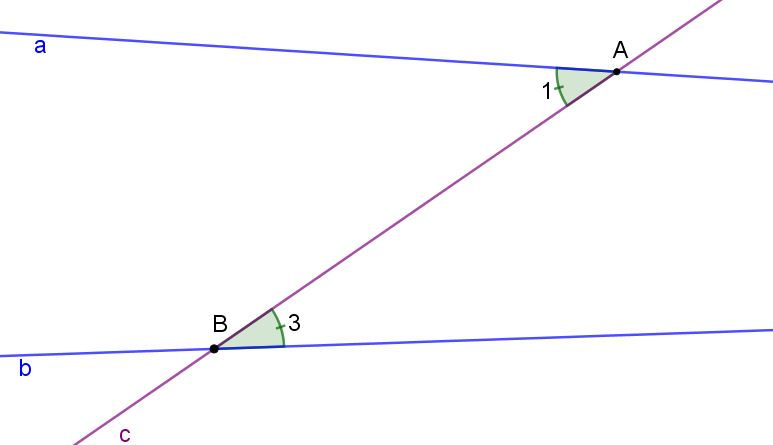
\includegraphics[width=0.5\linewidth]{figurenAuteur/zhoeken25}
\end{center}
\end{figure}

We zouden graag de eigenschap “verwisselende binnenhoeken zijn gelijk” gebruiken. Maar met de rechten $a$ en $b$ gaat dit niet, want de eigenschap werkt enkel als je evenwijdigen hebt.

\begin{werktekstoef}
\setcounter{enumi}{11}  

\item{Teken een extra rechte, zodanig dat je deze eigenschap wel kunt gebruiken. Laat zien dat dit tot iets onmogelijks leidt.}

\emph{De leerlingen tekenen bv. door $B$ een evenwijdige $d$ met $a$. Dan geldt:}
\begin{align}
\hat{B}_3 & = \hat{A}_1 & \emph{(gegeven)} \nonumber\\
 & = \hat{B}_3+\hat{B}_5 & \emph{(verwisselende binnenhoeken).} \nonumber
\end{align}


\emph{Maar dan moet} $$\hat{B}_5=0^\circ,$$
\emph{wat niet kan als $b$ niet evenwijdig is met $a$.}
\end{werktekstoef}

\begin{figure}[H]
\begin{center}
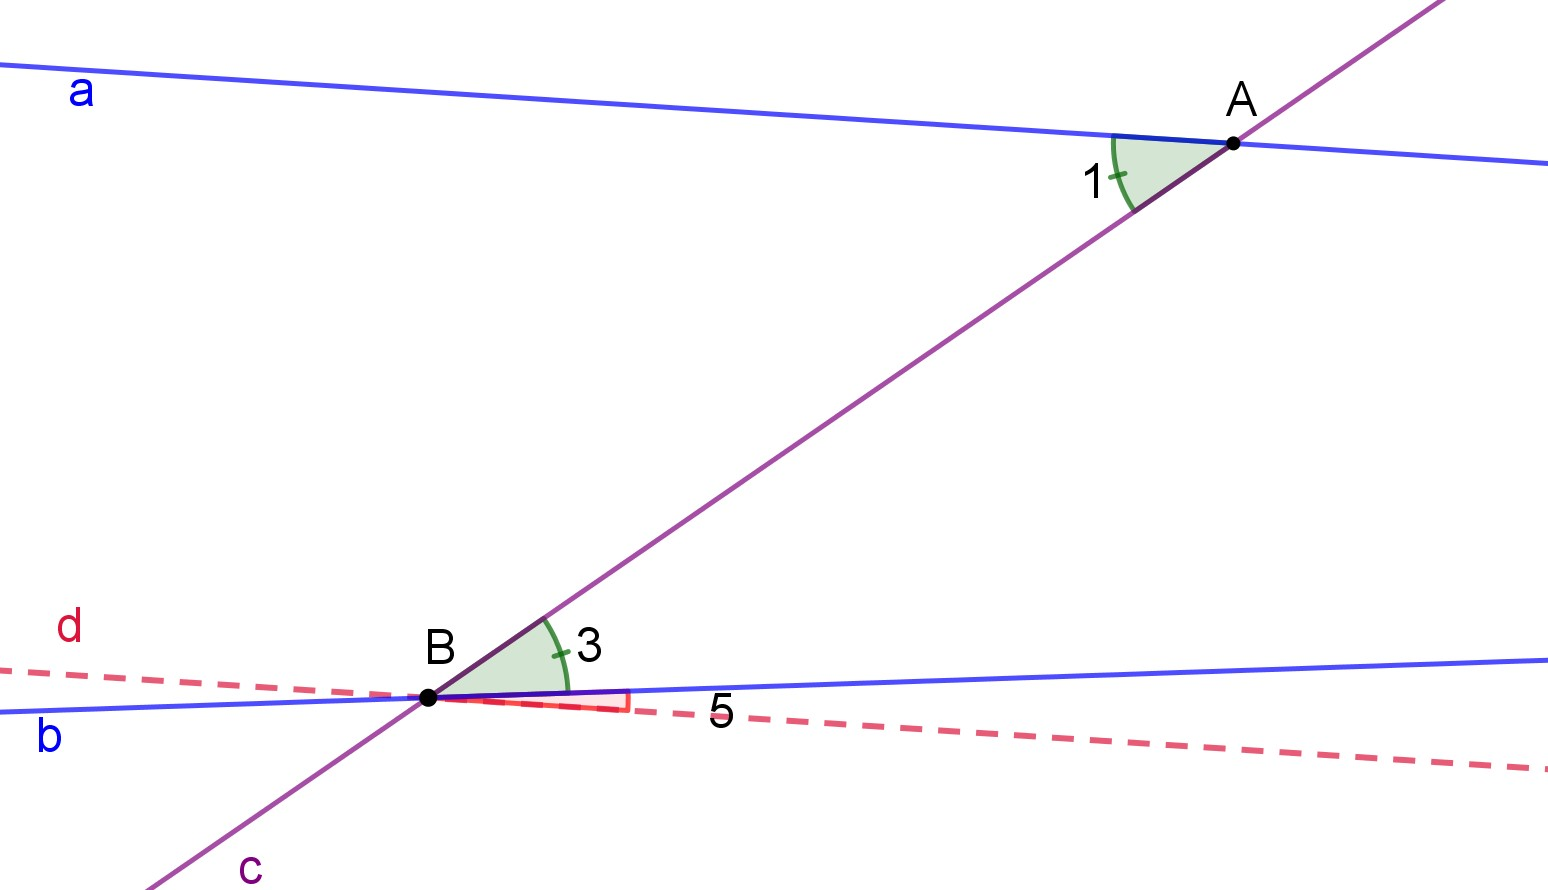
\includegraphics[width=0.6\linewidth]{figurenAuteur/zhoeken3}
\end{center}
\end{figure}

De veronderstelling dat $a$ en $b$ niet evenwijdig zijn, leidt dus tot onzin en kan niet waar zijn. Besluit: $a$ en $b$ zijn toch evenwijdig.

Bewijzen uit het ongerijmde komen vaak voor in de wiskunde. Men veronderstelt dat hetgeen men wil bewijzen niet waar is en men toont aan dat dit niet kan omdat het tot onzin leidt. Er is een minderheidsgroep wiskundigen die niet wil steunen op bewijzen uit het ongerijmde. Men noemt hen intuïtionisten.

Omdat zowel de eigenschap als de omgekeerde eigenschap gelden, kunnen we zeggen:
$$a\parallel b\Leftrightarrow \hat{A}_1=\hat{B}_3.$$

De dubbele pijl $\Leftrightarrow$ spreek je uit ``als en alleen als''. De enkele pijl wordt \emph{implicatie} genoemd en de dubbele pijl \emph{equivalentie}. 

Implicatie komt van het Latijn implicare: verwikkelen, insluiten (plica = vouw). Denk aan het Franse ``il est impliqué dans cette affaire'' (hij is bij deze zaak betrokken). In plaats van ``als $a//b$, dan $\hat{A}_1=\hat{B}_3$'' zeggen wiskundigen ook ``$a//b$ impliceert $\hat{A}_1=\hat{B}_3$''. Dit komt geleerder over.

Ook equivalentie komt van het Latijn. Aequus betekent gelijk en valere is kracht hebben, waard zijn, gelden, het Franse ``valoir''.

\eindewerktekst

\begin{multicols}{2}
Meteen na deze lesactiviteit zijn er eenvoudige oefeningen nodig om los te komen van de vaste notaties. Leerlingen mogen niet de indruk krijgen dat bv. overeenkomstige hoeken noodzakelijk dezelfde index moeten hebben (zoals $\hat{A}_1$ en $\hat{B}_1$)...
Voor leerlingen die toe zijn aan wat creatievere (bewijs-)oefeningen hierover, vermelden we er enkele.

\begin{opsomming}
\item Wat is het verband tussen twee opeenvolgende hoeken van een parallellogram? Bewijs dit verband.

\item (Naar Schmid \& Schweitzer, 1990.) De visser (zie figuur\ref{visser3}) wordt een beetje moe en laat zijn hengel (dit is de stok waaraan de vislijn bevestigd is) zakken over een hoek $\alpha$. De hoek $\beta$ verandert hierdoor in de hoek $\gamma$, die groter is dan $\beta$. Hoeveel groter? Bewijs dat.

\begin{figure}[H]
\begin{center}
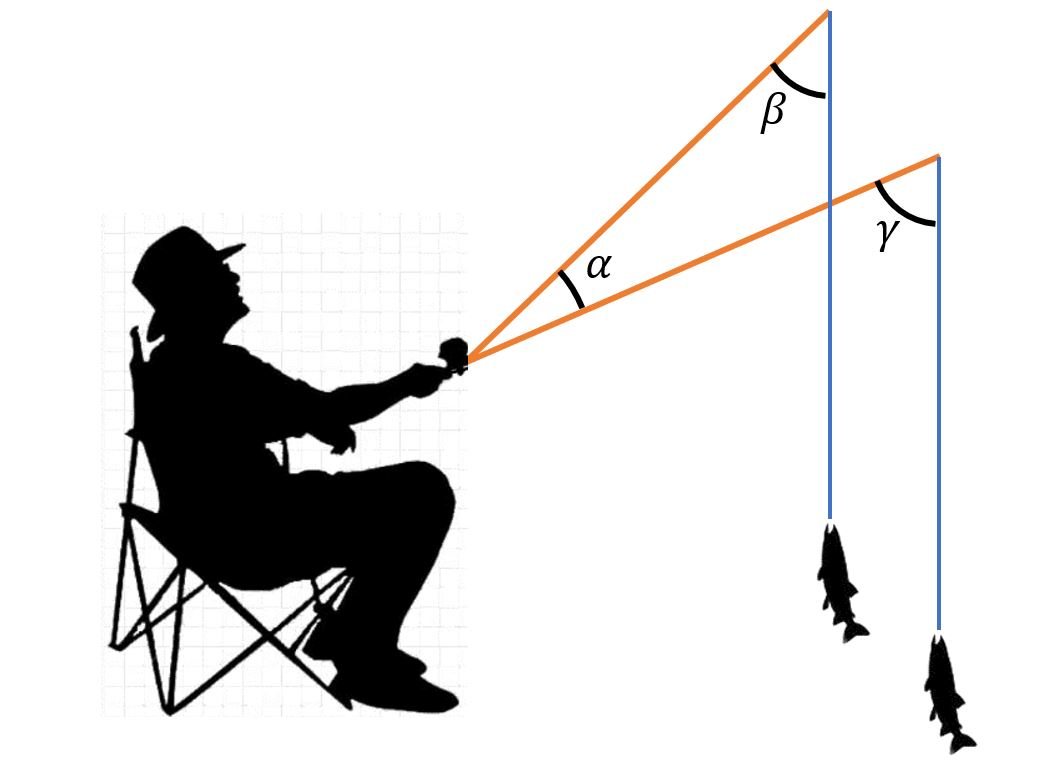
\includegraphics[width=0.9\linewidth]{figurenAuteur/visser3}
\captionof{figure}{De visser: opgave}
\label{visser3}
\end{center}
\end{figure}

\emph{Een mogelijke werkwijze wordt gesuggereerd door figuur \ref{visser4}. Dit geeft: $\gamma=\alpha+\beta$. Het is ook mogelijk om te steunen op de som van de hoeken van een driehoek.}

\begin{figure}[H]
\begin{center}
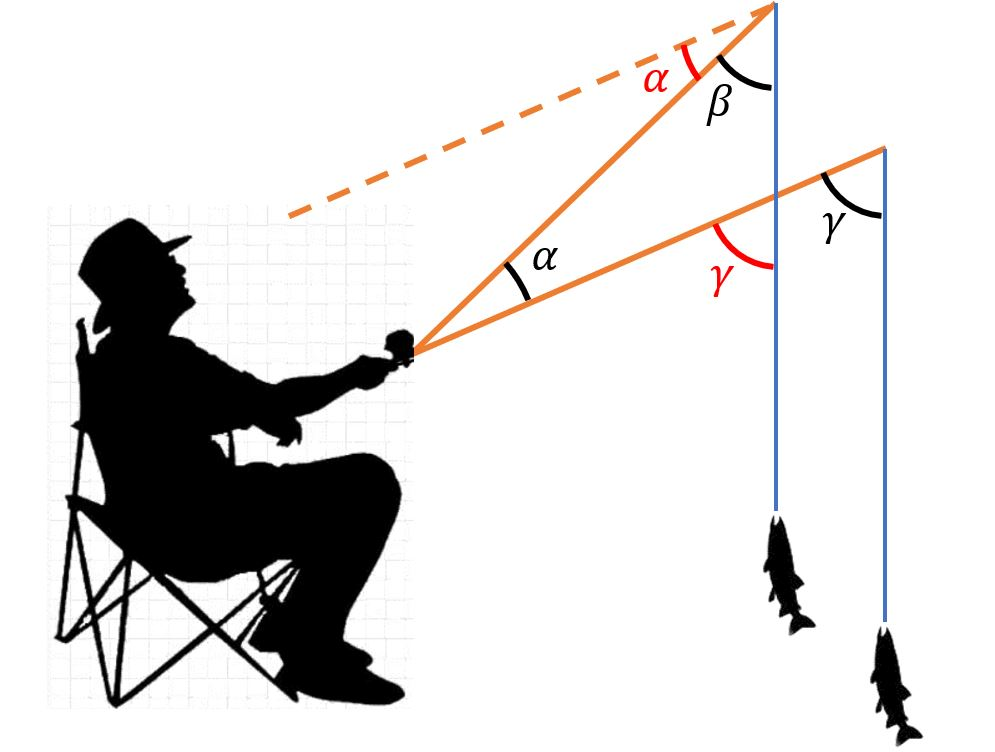
\includegraphics[width=0.86\linewidth]{figurenAuteur/visser4}
\captionof{figure}{De visser: mogelijke werkwijze}
\label{visser4}
\end{center}
\end{figure}

\item In figuur \ref{oefbiss} zijn $AC$ en $BD$ evenwijdig en is hoek $\alpha$ willekeurig. $BC$ is de bissectrice van $A\hat{B}D$ en $CD$ is de bissectrice van de hoek tussen $[BC]$ en het verlengde van $AC$. Maak een nieuwe tekening waarbij de hoek $\alpha$ groter of kleiner is dan op deze figuur. Onderzoek wat het verband is tussen de hoeken $\alpha$ en $\beta$.

\emph{Het verband is $\beta=\frac {\alpha}{4}+45^\circ$.}

\begin{figure}[H]
\begin{center}
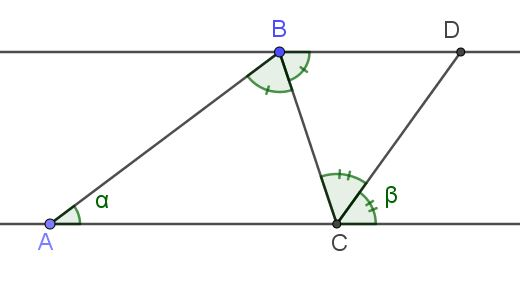
\includegraphics[width=0.7\linewidth]{figurenAuteur/oefbiss}
\captionof{figure}{Bissectrices}
\label{oefbiss}
\end{center}
\end{figure}

\end{opsomming}
\end{multicols}
\begin{center}
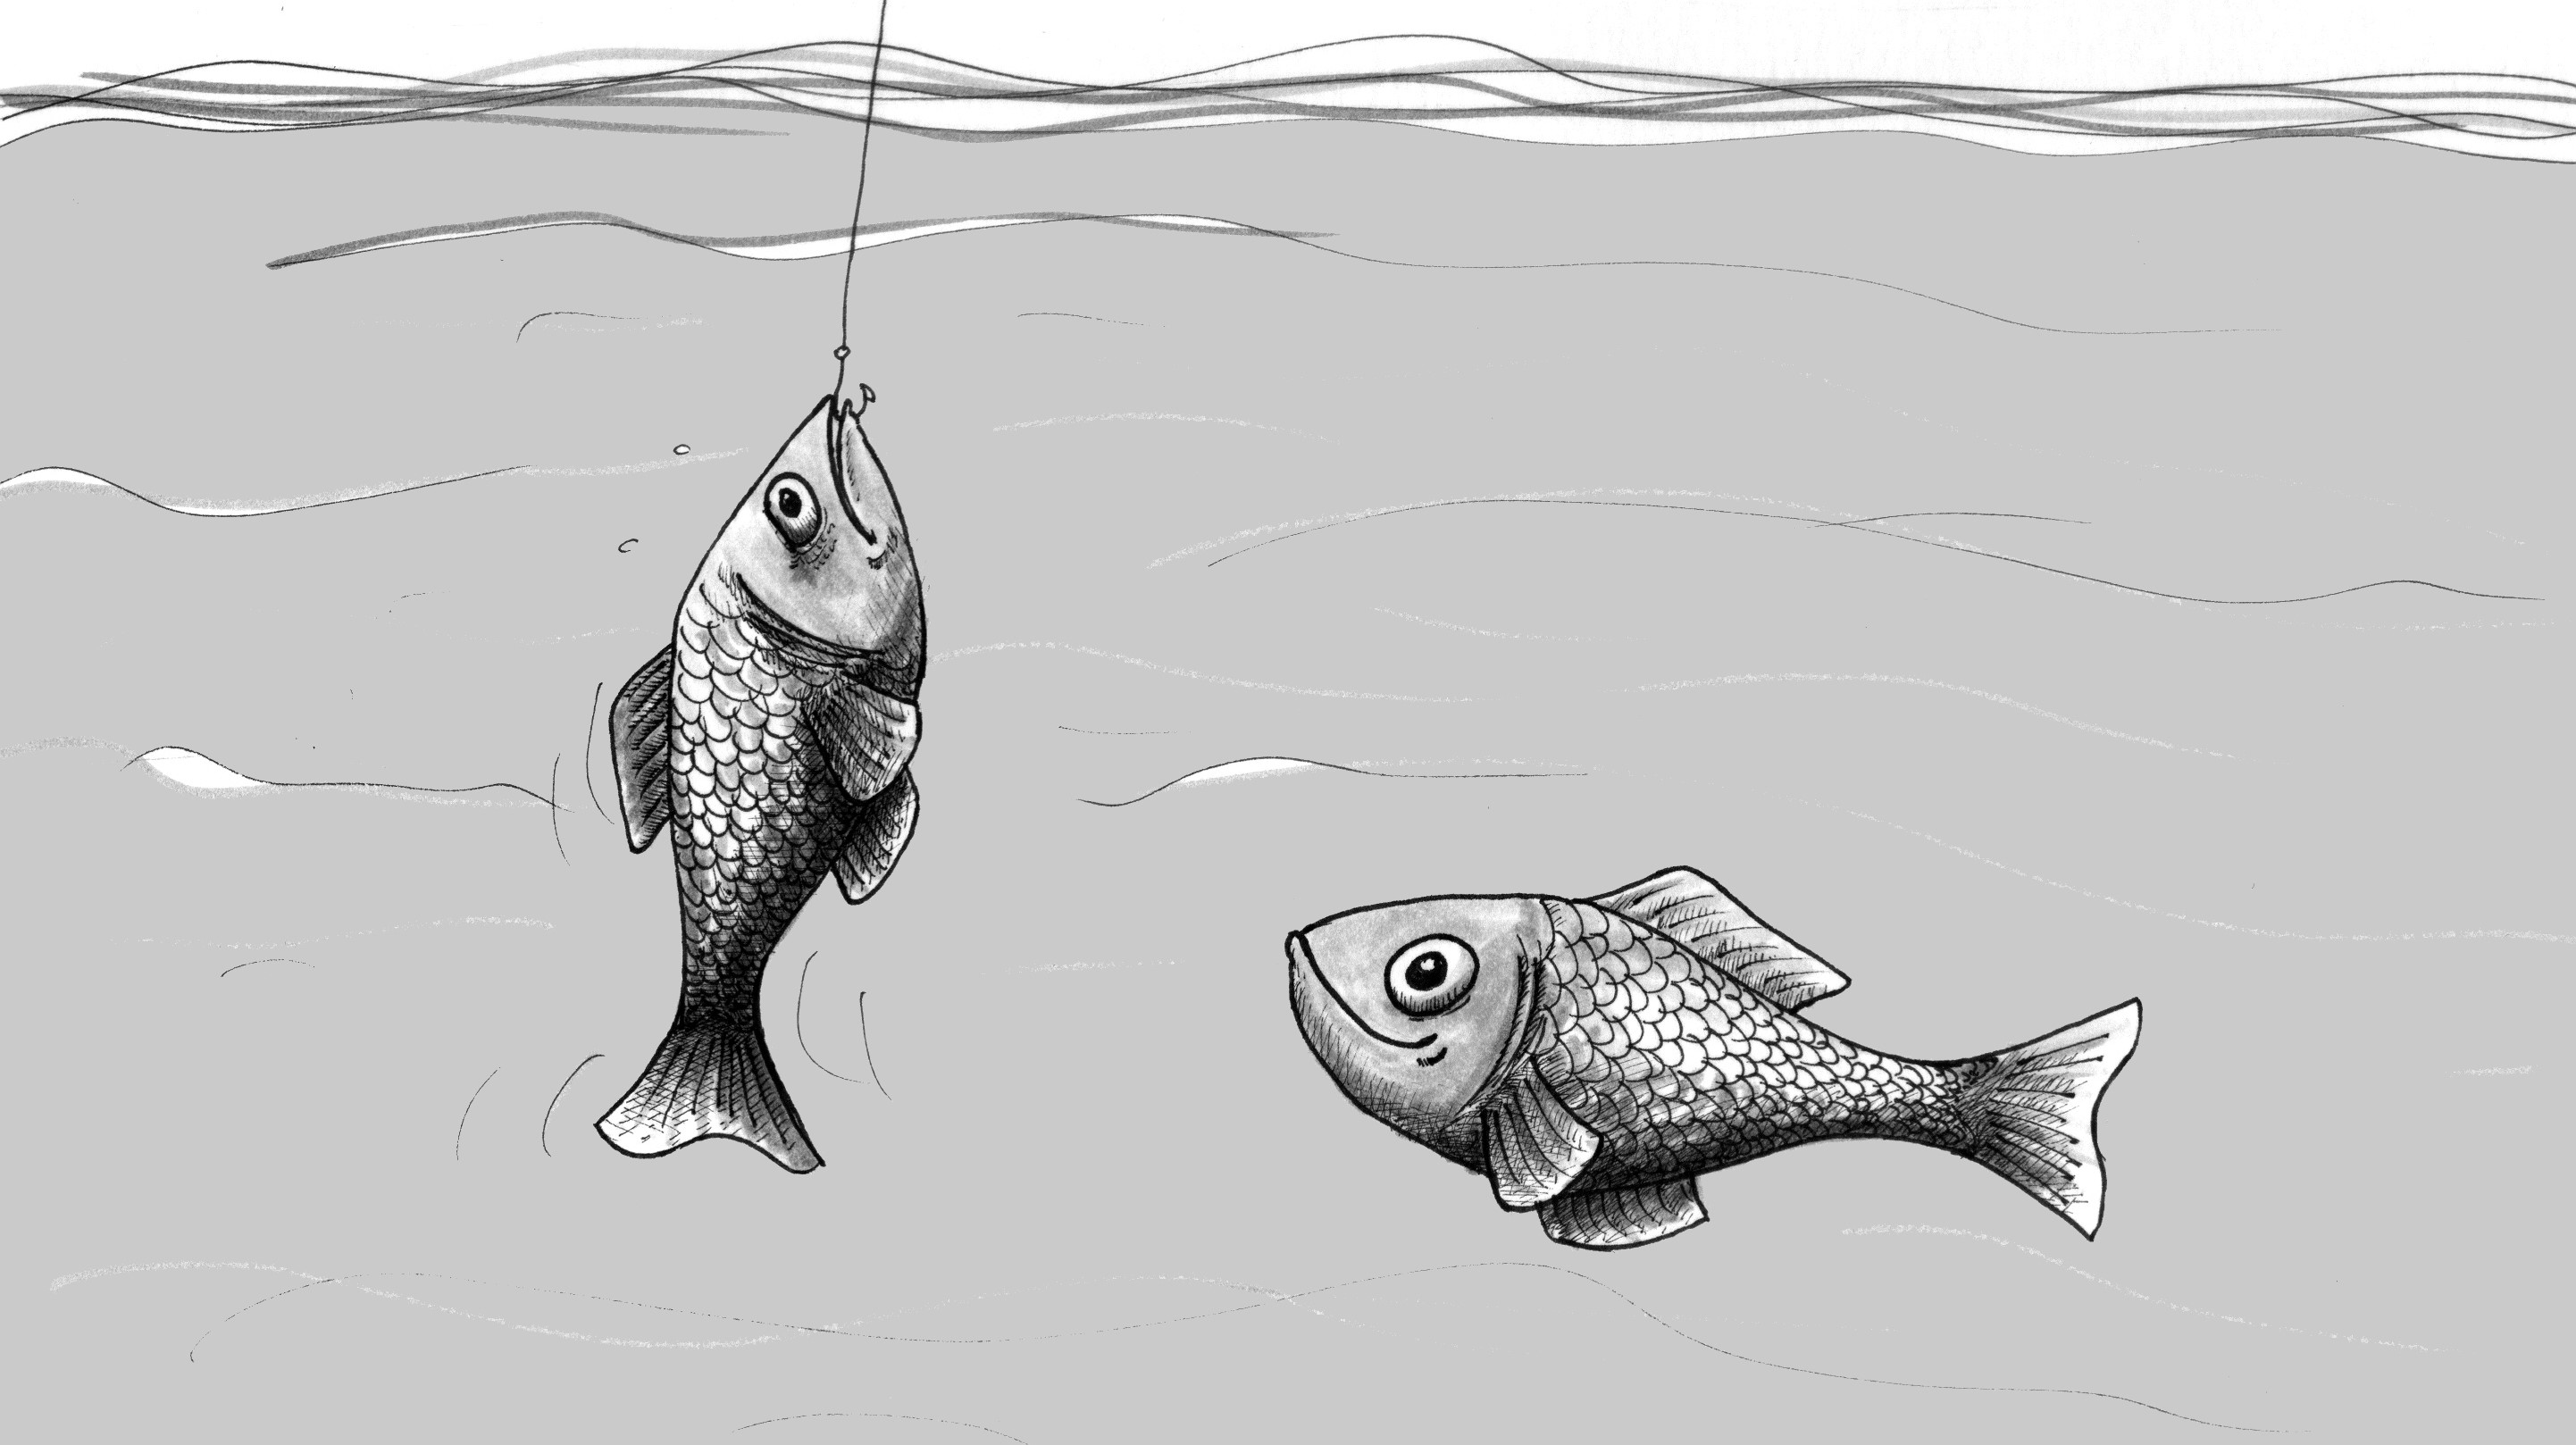
\includegraphics[width=0.85\linewidth]{tekeningenKurt/vissen.jpg}
\end{center}
\begin{multicols}{2}
\subsection{Som van de hoeken}
Als je een zijde en de twee aanliggende hoeken van een driehoek kent, ligt de derde hoek vast. Deze vaststelling geeft aan dat er een verband moet zijn tussen de hoekgroottes van de drie hoeken. Leerlingen kunnen de hoeken meten en optellen. Afhankelijk van de meetnauwkeurigheid zullen ze iets in de buurt van 180° uitkomen. Dit bewijst nog niet dat de som 180° is; het zou bv. ook 179,9° kunnen zijn.

In de lesactiviteit hieronder bewijzen de leerlingen op drie manieren dat de som van de hoeken van een driehoek gelijk is aan 180°. \\
Je kunt de klas in drie groepen verdelen en door elke groep één bewijs laten uitwerken en nadien aan de anderen laten uitleggen. De lesactiviteit zet op weg om het bewijs te vinden. Daarna is het nuttig om de leerlingen het bewijs netjes te laten uitschrijven (niet meer met vragen en antwoorden).

\end{multicols}


\beginwerktekst{Som van de hoeken van een driehoek}

\tussentitel{Het scheurbewijs}

Teken een willekeurige driehoek $ABC$. Geef elke hoek een andere kleur. Scheur de hoeken $\hat{A}$ en $\hat{B}$ en plaats ze tegen de hoek $\hat{C}$ zodat ze aanliggende hoeken worden.

\begin{figure}[H]
\begin{center}
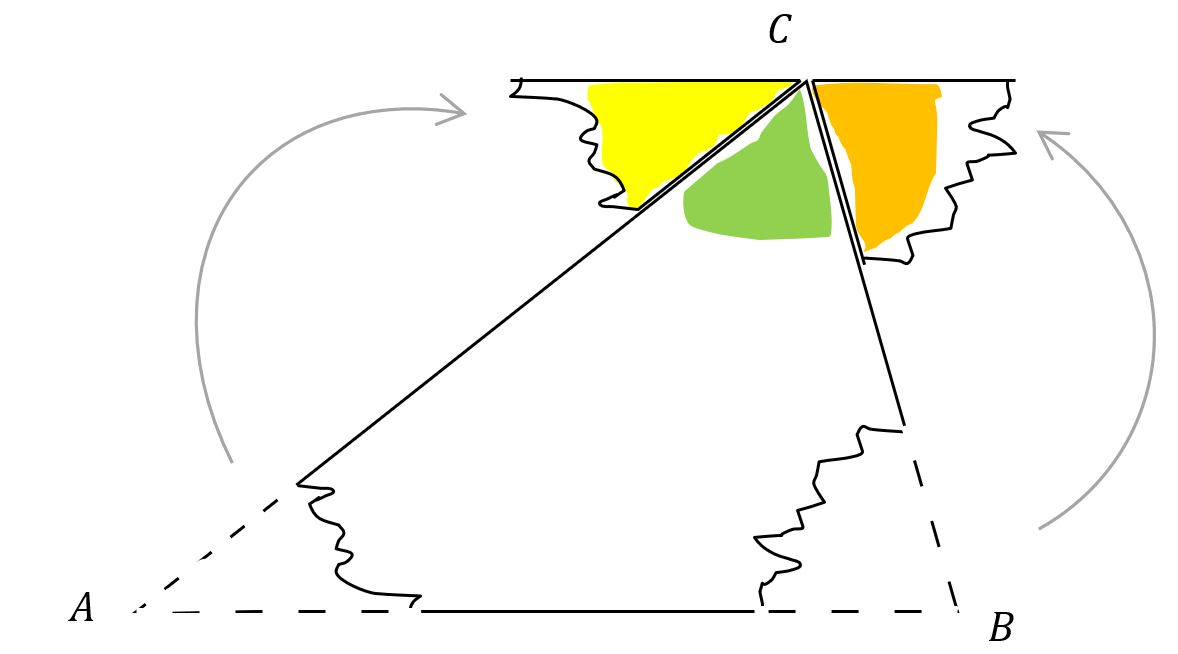
\includegraphics[width=0.47\linewidth]{figurenAuteur/hoekensom}
\end{center}
\end{figure}
\begin{werktekstoef}

\item Druk het ``scheuren en verplaatsen'' van de hoeken $\hat{A}$ en $\hat{B}$ op een wiskundige manier uit: wat construeer je precies?

\emph{We construeren tegen de driehoek (aan de linkerkant) een hoek met hoekpunt $C$ en been $[CA$ die even groot is als de hoek $\hat{A}$}. Analoog construeren we aan de rechterkant een hoek met hoek punt $C$ en been $[CB$ even groot als $\hat{B}$.

\item Wat moet je over je geconstrueerde hoeken bewijzen om aan te tonen dat de som van de drie hoeken 180° is?

\emph{We moeten bewijzen dat de bijgetekende benen van de hoeken in $C$ doorlopen, met andere woorden dat het halfrechten zijn van een zelfde rechte.}

\item Hoe bewijs je dat?

\emph{Beide halfrechten zijn evenwijdig met $AB$ door ``verwisselende binnenhoeken omgekeerd''. Omdat er door $C$ maar één rechte bestaat die evenwijdig is met $AB$, liggen beide halfrechten op dezelfde rechte. Dus: de som is 180°.}

\end{werktekstoef}

\tussentitel{Het bewijs met een evenwijdige}

Teken een rechte door $C$ evenwijdig met $AB$.\
\begin{figure}[H]
\begin{center}
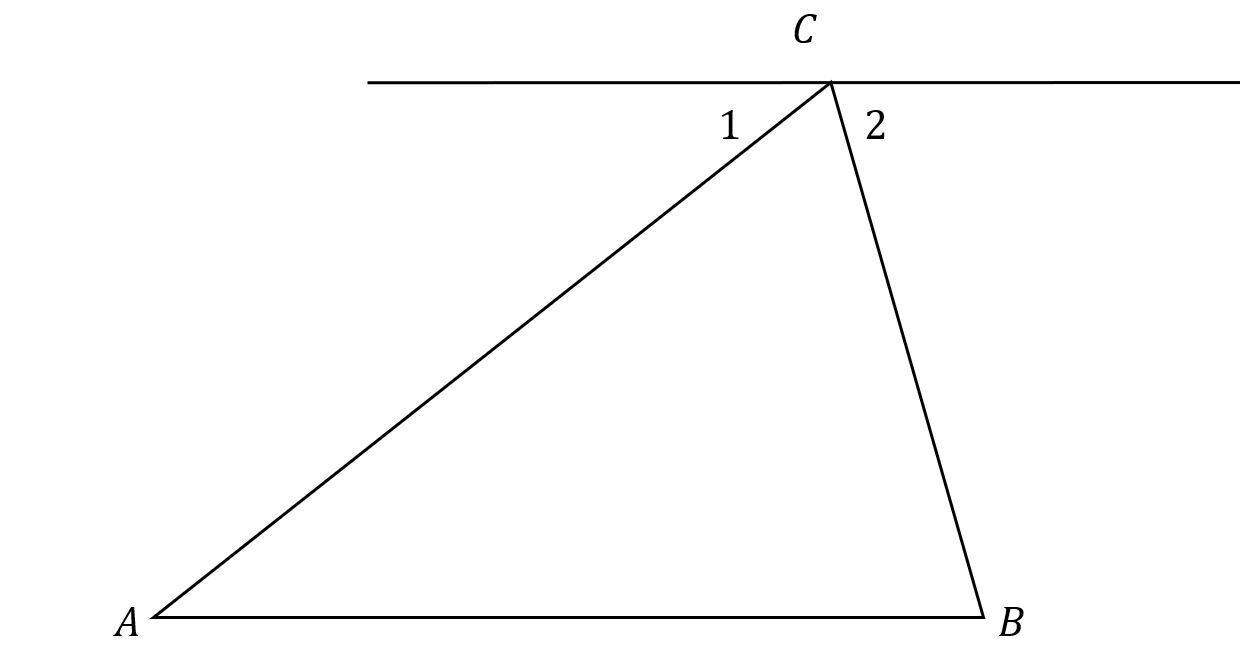
\includegraphics[width=0.50\linewidth]{figurenAuteur/hoekensom2}
\end{center}
\end{figure}
\begin{werktekstoef}
\setcounter{enumi}{3} 
\item Welke hoeken zijn gelijk en waarom?

\emph{De hoek $\hat{C_1}$ (zie figuur) is gelijk aan $\hat{A}$ en de hoek $\hat{C_2}$ is gelijk aan $\hat{B}$, wegens verwisselende binnenhoeken.}



\item Werk het bewijs af: waarom volgt hieruit dat de som van de hoeken van de driehoek 180° is?

\emph{De som van de hoeken van de driehoek $\hat{A}+\hat{B}+\hat{C}$ is gelijk aan $\hat{C_1}+\hat{C_2}+\hat{C}$ en dat is 180°.}
\end{werktekstoef}
\tussentitel{Het bewijs met een telegeleide auto}

Veronderstel dat je het autootje op de figuur hieronder vanop afstand kunt besturen. Je hebt een knop om die vooruit te laten rijden en je hebt een wieltje om die te laten draaien. Het is een fictieve auto en die draait ook een beetje anders dan echte auto's. Als die draait, gebeurt dit rond het midden van zijn achterbumper. 

\begin{werktekstoef}
\setcounter{enumi}{5} 
\item Stel dat je de auto vooruit laat rijden vanuit de positie op de figuur, tot het midden van de achterbumper in het volgende hoekpunt staat. Over welke hoek moet je de auto laten draaien zodat die op de volgende zijde verder kan rijden?

\emph{Het supplement van de hoek van de driehoek in dat hoekpunt.}

\begin{figure}[H]
\begin{center}
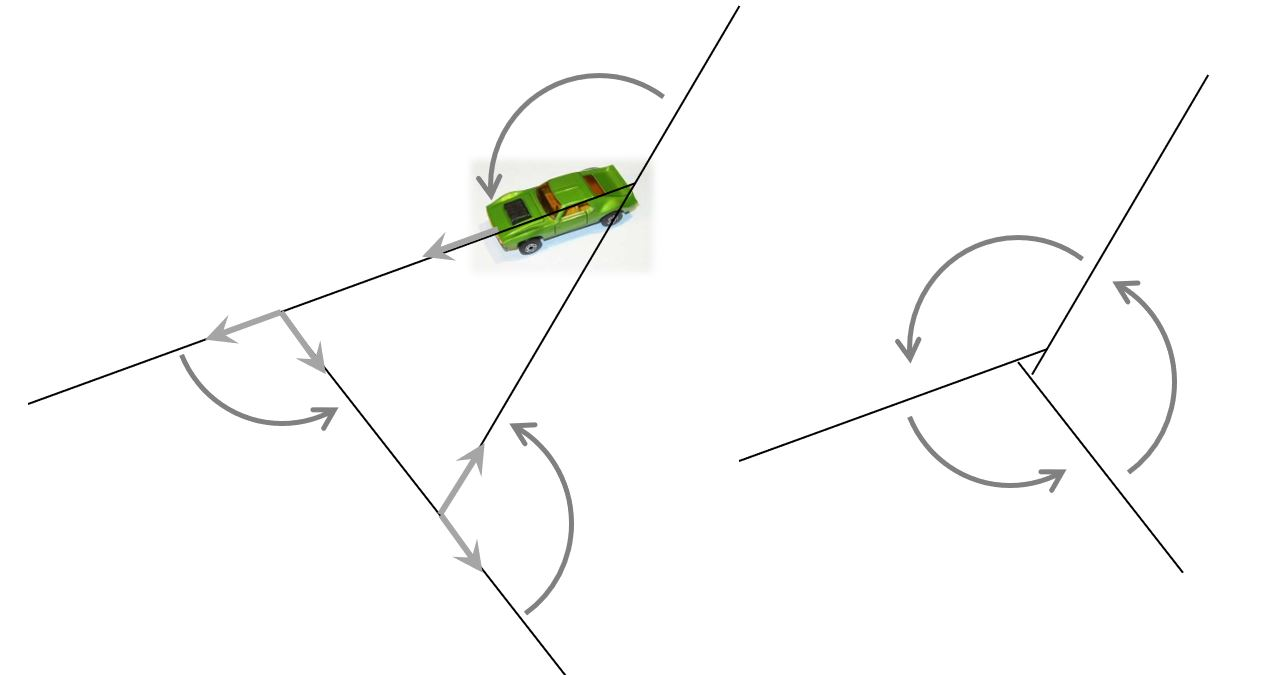
\includegraphics[width=0.68\linewidth]{figurenAuteur/hoekensomautootje}
\end{center}
\end{figure}

\item Laat de auto op die manier helemaal rond de driehoek rijden, tot hij weer in de beginpositie staat. Over hoeveel graden heeft het autootje in totaal gedraaid? Tip: laat in gedachten de driehoek piepklein worden zoals op de figuur ernaast.

\emph{De auto is gedraaid over een volle hoek (360°). Het verkleinen van de driehoek zorgt voor wat psychologen een `Gestalt' noemen: eens je het ziet, kun je het niet meer niet zien... Als (overkritische) leerlingen het kijken naar een `piepkleine' driehoek nog niet overtuigend genoeg vinden, kunnen ze ook meteen het limietgeval creëren: een punt tekenen en vanuit dit punt halfrechten evenwijdig met de benen van de hoeken waarover de auto draait. De som van deze hoeken is gelijk aan 360°.}
\newpage
\item Maak het bewijs af: waarom bewijst dit dat de som van de hoeken van de driehoek gelijk is aan 180°?

\emph{De som van de supplementen van de hoeken van de driehoek is 360°. Dit geeft}
\begin{align}
180^\circ-\hat{A}+180^\circ-\hat{B}+180^\circ-\hat{C}&=360^\circ \nonumber \\
\hat{A}+\hat{B}+\hat{C}&=180^\circ \nonumber
\end{align}
\end{werktekstoef}
\eindewerktekst
\begin{multicols}{2}

De leerlingen kunnen, steunend op de som van de hoeken in een driehoek, de som van de hoeken in een vierhoek, vijfhoek, ... $n$-hoek zoeken. Een mogelijke werkwijze is het tekenen van diagonalen vanuit één hoekpunt. Op die manier wordt een vierhoek verdeeld in twee driehoeken, een vijfhoek in drie driehoeken, ... een $n$-hoek in $n-2$ driehoeken. Op die manier is de som van de hoeken van een vierhoek $360^\circ$, van een vijfhoek $540^\circ$, ... van een $n$-hoek $(n-2)\cdot 180^\circ$. Verdelen de leerlingen de veelhoek in driehoeken vanuit een centraal punt binnen de veelhoek, dan verdelen ze hiermee de $n$-hoek in $n$ driehoeken, maar hierbij creëren ze een overtollige volle hoek die nog van de som $n\cdot 180^\circ$ moet worden afgetrokken om de som van de hoeken van de $n$-hoek te verkrijgen.

Een mooie context waarin de som van de hoeken van veelhoeken tot zijn recht komt, is `betegelingen'. We verwijzen hiervoor naar Van Leemput \& Roelens (2006).

Een wat zwaardere oefening op de som van de hoeken in veelhoeken gaat over een stervijfhoek.

\begin{quote}

 Bepaal de som van de `uitspringende' hoeken van de stervijfhoek (figuur \ref{stervijfhoek}).    
\end{quote}
\begin{figure}[H]
\begin{center}
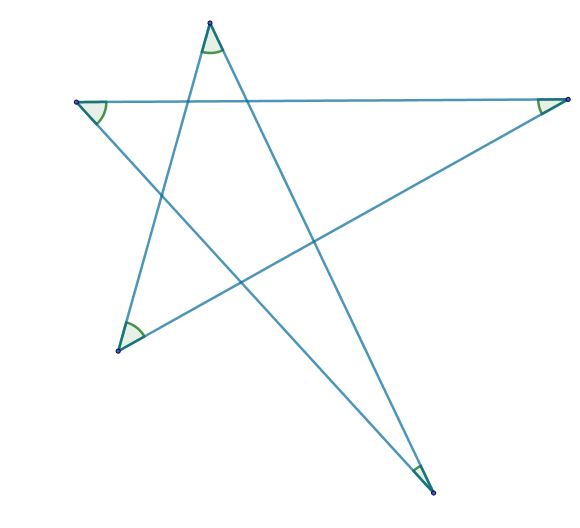
\includegraphics[width=0.80\linewidth]{figurenAuteur/stervijfhoek1}
\captionof{figure}{Stervijfhoek}
\label{stervijfhoek}
\end{center}
\end{figure}
Met GeoGebra of door goed te meten komen de leerlingen er snel achter dat de som gelijk is aan 180°, maar om het te bewijzen moeten ze systematisch te werk gaan. We zetten de lezer op weg zonder alle details uit te schrijven.
\end{multicols}
\begin{center}
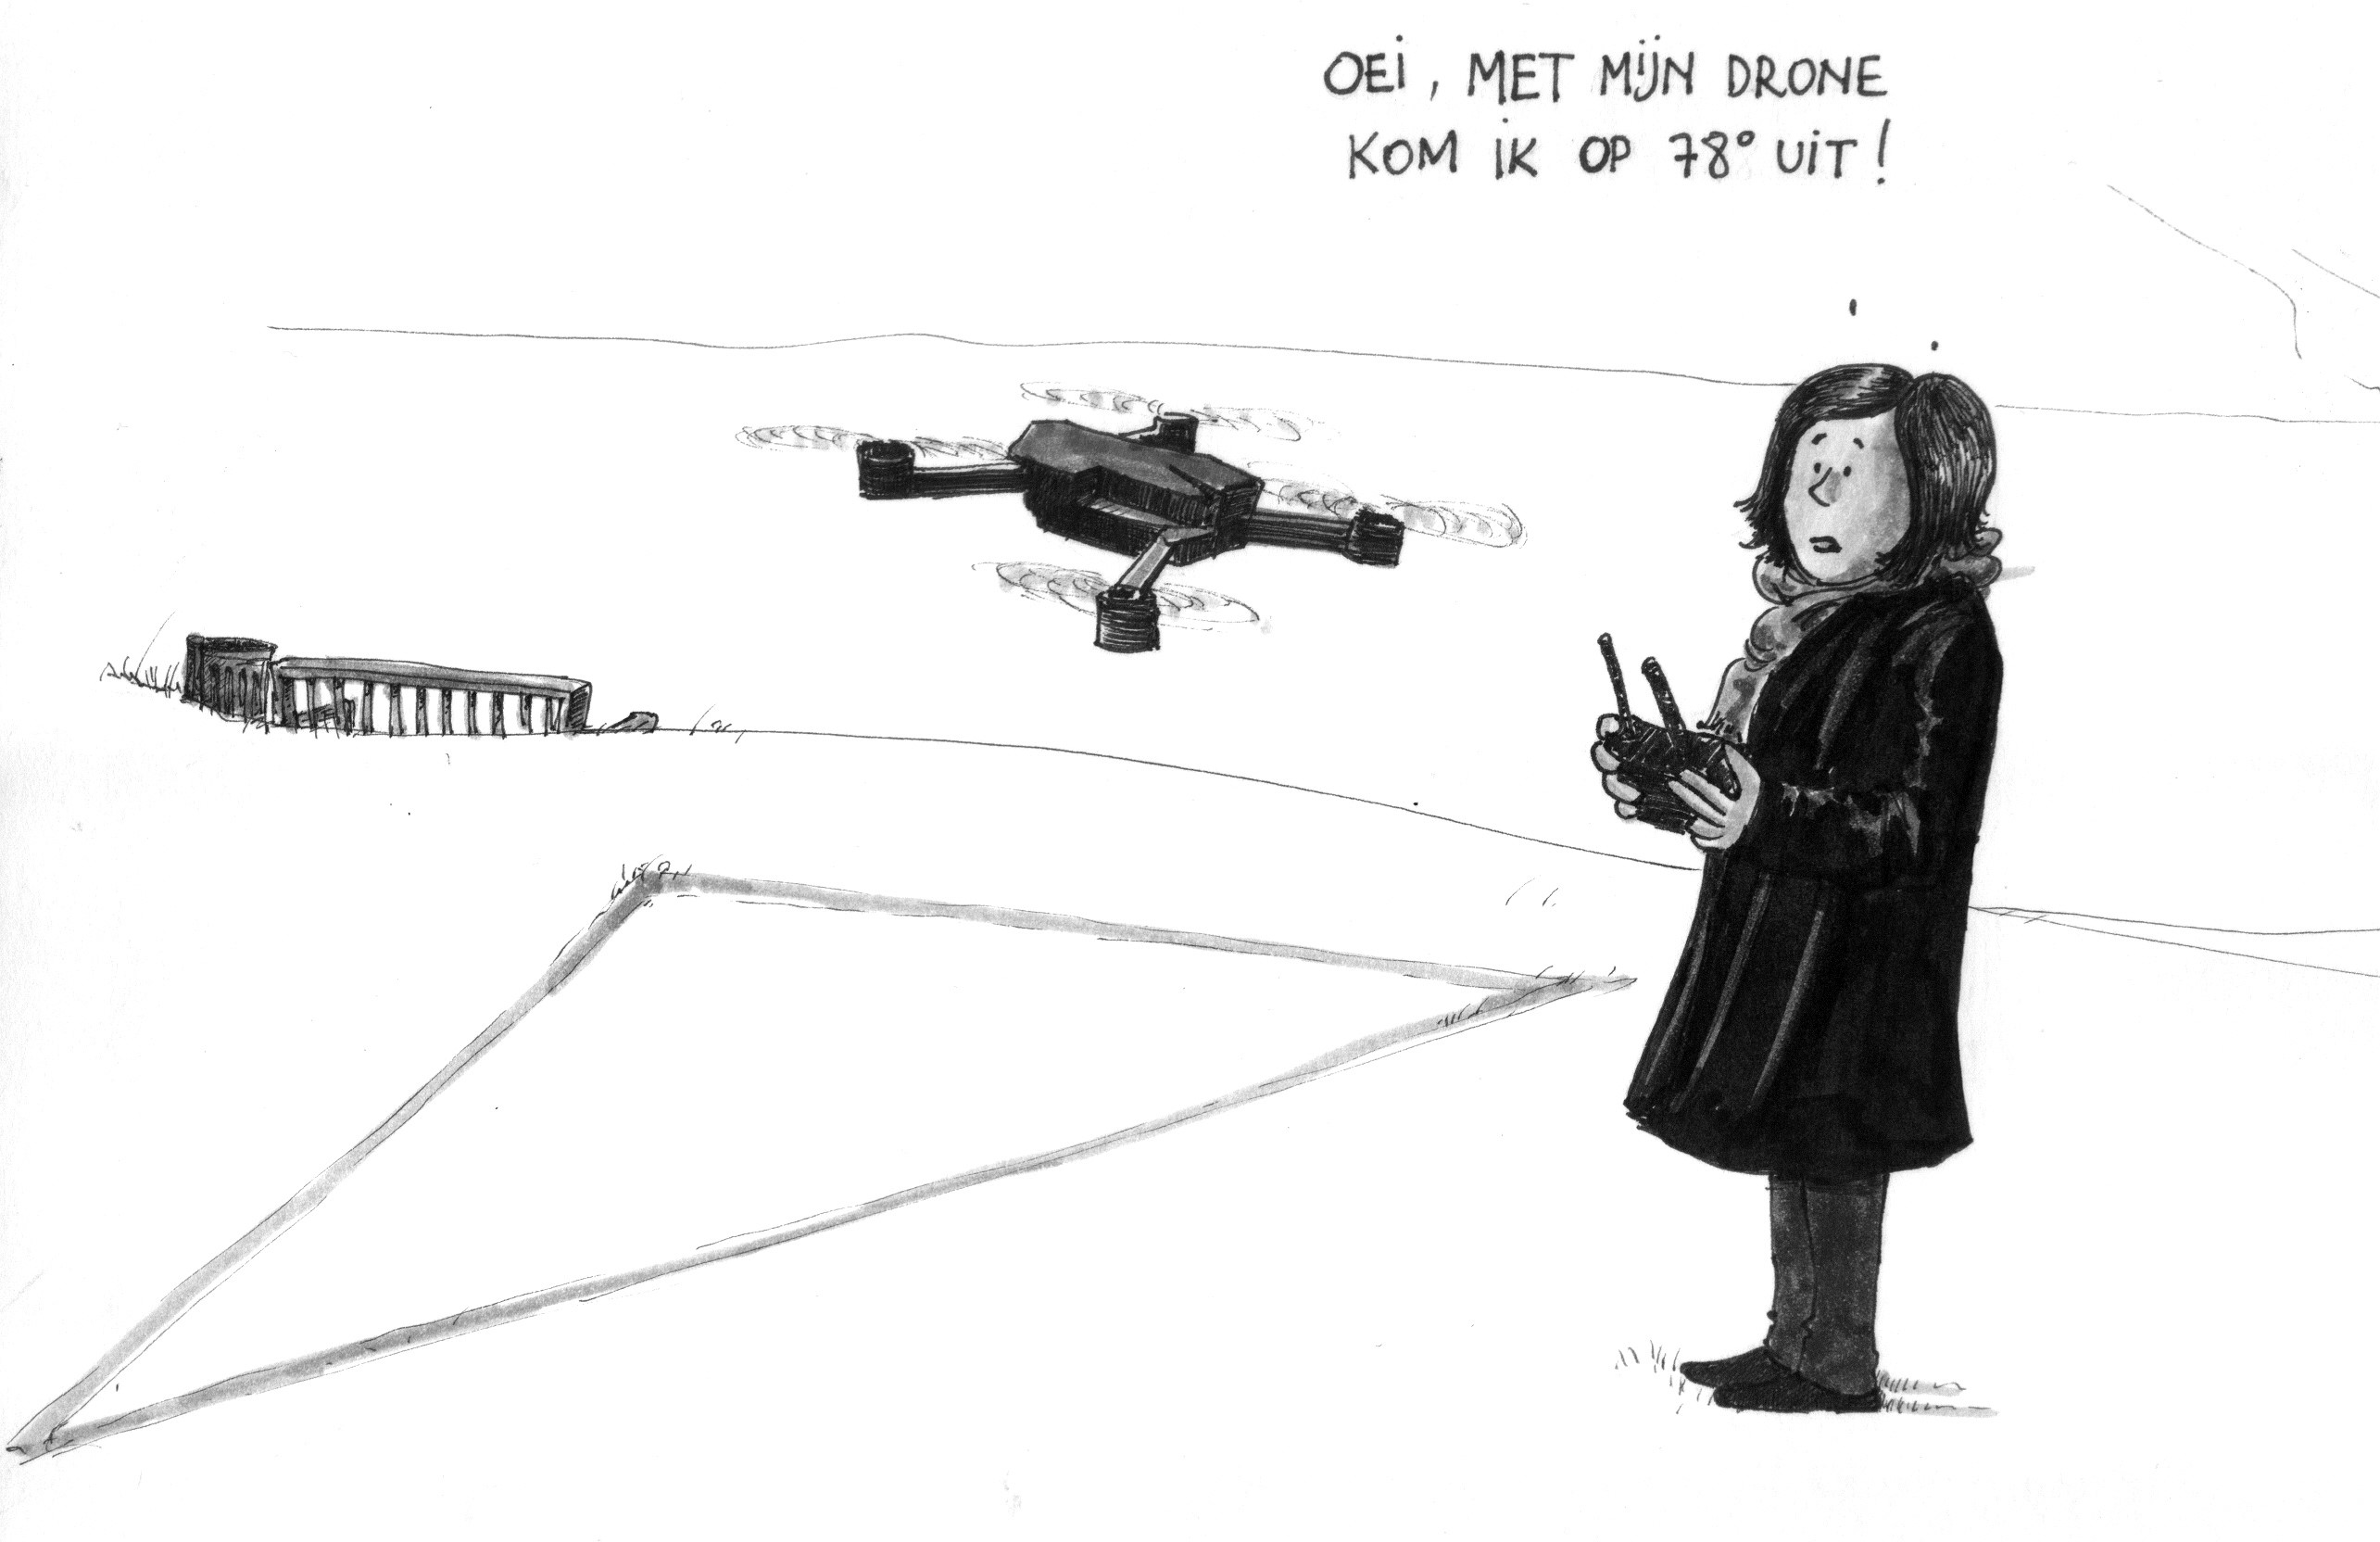
\includegraphics[width=0.75\linewidth]{tekeningenKurt/drone.jpg}
\end{center}
\begin{multicols}{2}
\begin{opsomming}
\item Ze kunnen werken met driehoeken gevormd door één hoek van de binnenste vijfhoek en twee `uitsteeksels'. Als ze van de som van de hoeken van deze vijf driehoeken ($5\cdot 180^\circ$) de som van de hoeken van de binnenste vijfhoek ($3\cdot 180^\circ$) aftrekken, dan moeten ze nog delen door twee want ze hebben elke aangeduide hoek twee keer geteld. 
\item Ze zouden ook kunnen werken met de vijf buitenste driehoeken. De som is $5\cdot 180^\circ$, waarvan ze twee keer de som van de buitenhoeken van de binnenste vijfhoek moeten aftrekken want die zijn teveel geteld. 

\item Ook het telegeleid autootje kan hier heel nuttig zijn om een kort bewijs op te stellen. De auto maakt in totaal twee verschillende wentelingen ($4 \cdot 180^\circ$) en dus blijft er om 5 gestrekte hoeken te maken nog $180^\circ$ over voor de hoeken van de ster (zie figuren \ref{stervijfhoekauto1} en \ref{stervijfhoekauto2}).
\end{opsomming}

\begin{figure}[H]
\begin{center}
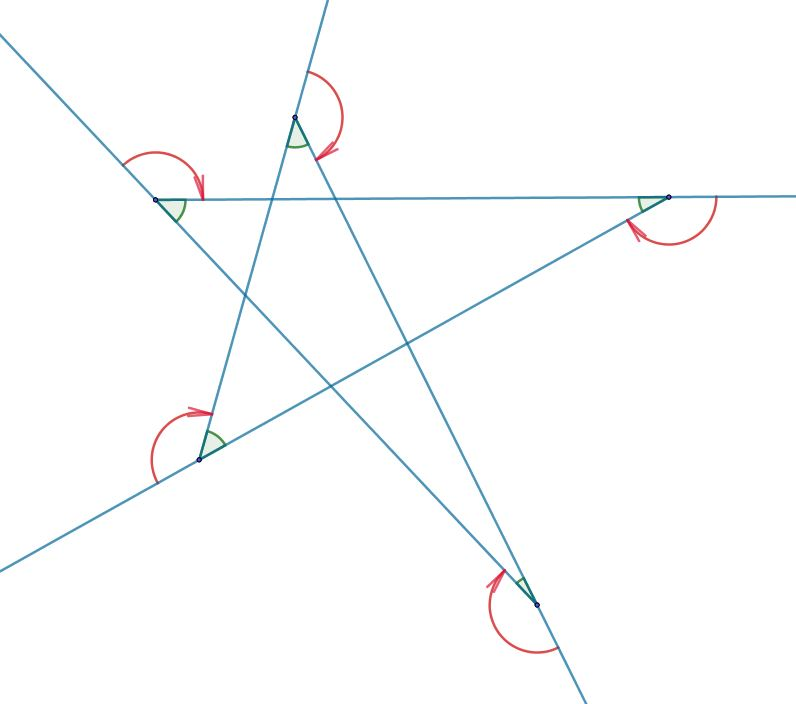
\includegraphics[width=0.9\linewidth]{figurenAuteur/stervijfhoekauto1}
\captionof{figure}{Autootje langs de stervijfhoek}
\label{stervijfhoekauto1}
\end{center}
\end{figure}

\begin{figure}[H]
\begin{center}
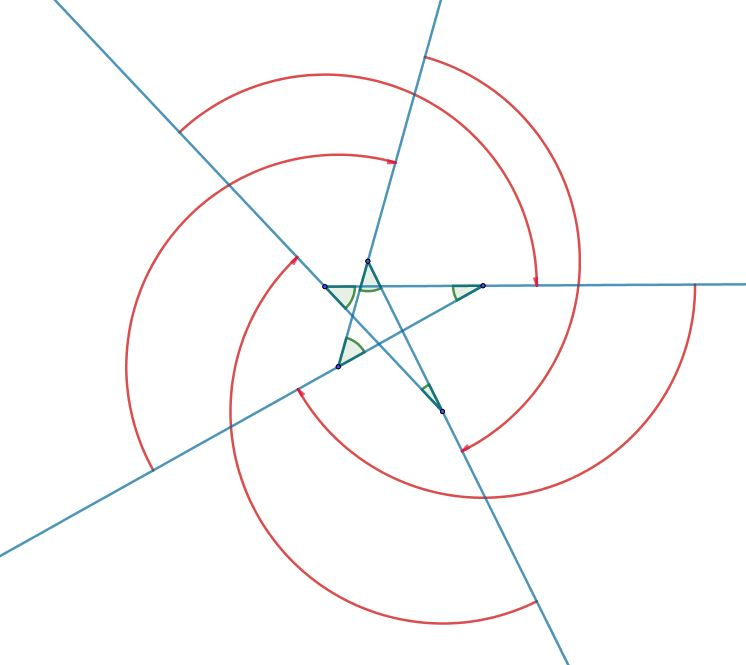
\includegraphics[width=0.9\linewidth]{figurenAuteur/stervijfhoekauto2}
\captionof{figure}{Autootje langs de stervijfhoek, uitgezoomd}
\label{stervijfhoekauto2}
\end{center}
\end{figure}

\section{Bewijzen met congruente driehoeken}

Het gebruik van congruente driehoeken om te bewijzen dat lijnstukken even lang zijn of dat hoeken even groot zijn, is niet nieuw en kreeg ook in het huidige leerplan veel aandacht. Omdat dit bij de lezers erg bekend is, werken we hier geen lesactiviteiten uit, maar beperken we ons tot enkele ideeën die we willen benadrukken.

Het voordeel van congruentiekenmerken is dat het voor de bewijzende leerling een duidelijk kader biedt. 

Om te bewijzen dat twee lijnstukken even lang zijn (voor twee hoeken is het analoog), moet je op zoek gaan naar twee driehoeken waarbij het ene lijnstuk een zijde is van de ene driehoek en het andere lijnstuk een zijde is van de andere driehoek. Uiteraard moet je geen driehoeken nemen waarvan je meteen ziet dat ze niet congruent kunnen zijn (een `korte dikke' en een `lange magere' maken geen kans...). Soms moet je iets bijtekenen omdat de geschikte driehoeken nog niet voorhanden zijn. Vervolgens moet je, steunend op wat gegeven is, aantonen dat één van de congruentiekenmerken geldig is: een voldoende voorwaarde voor congruentie. De congruentiekenmerken van driehoeken bestaan uit drie gelijkheden (zzz, zhz, hzh, hhz, zz90°). 

Merk op: zzh is geen congruentiekenmerk omdat het soms mogelijk is om twee driehoeken te tekenen die aan deze voorwaarden voldoen maar niet congruent zijn. In figuur \ref{zzh2} probeer ik een driehoek met $5,7, 40^\circ$ te maken, in die volgorde. Ik teken een lijnstuk van lengte 7 en aan één uiteinde hiervan een hoek van $40^\circ$. Aan het andere uiteinde moet een zijde van lengte 5 komen. Met de passer zie ik dat er twee mogelijkheden zijn voor het derde hoekpunt en deze mogelijkheden leveren driehoeken met $5, 7, 40^\circ$ op die niet congruent zijn.

\begin{figure}[H]
\begin{center}
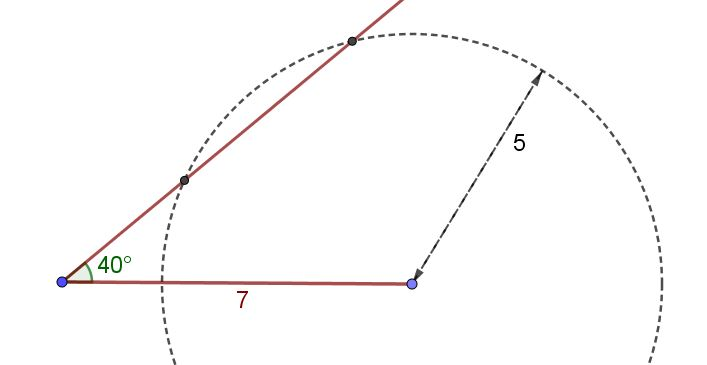
\includegraphics[width=0.95\linewidth]{figurenAuteur/zzh2}
\captionof{figure}{}
\label{zzh2}
\end{center}
\end{figure}

Wanneer de hoek tegenover de langste van deze twee zijden staat, dan kan dit niet. In figuur \ref{zzh} probeer ik een driehoek met $7,5, 40^\circ$ te maken en nu is er maar één mogelijkheid. De cirkel snijdt de halfrechte maar in één punt. Zzh (lange zijde, korte zijde, hoek) is wel een congruentiekenmerk. 

\begin{figure}[H]
\begin{center}
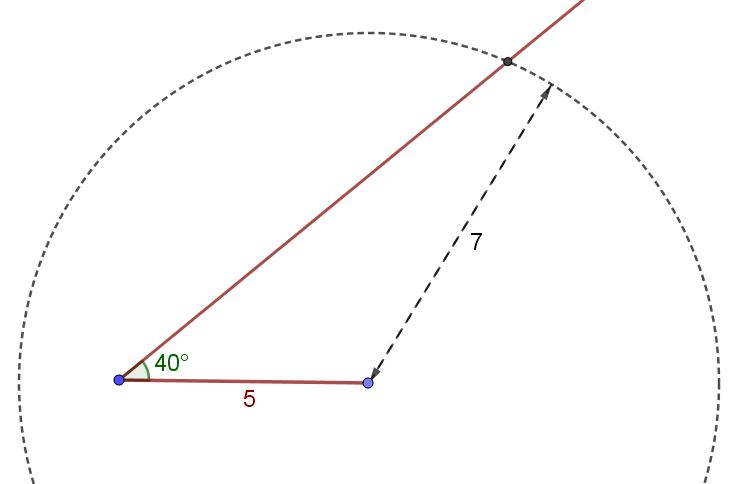
\includegraphics[width=0.95\linewidth]{figurenAuteur/zzh}
\captionof{figure}{}
\label{zzh}
\end{center}
\end{figure}
In het secundair onderwijs wordt hiervan meestal enkel het speciale geval zz90° vermeld. Het is een speciaal geval van Zzh want de schuine zijde is inderdaad altijd langer dan één van de rechthoekszijden.

We pleiten ervoor om genoeg aandacht te besteden aan het `zoeken' van zo'n bewijs en niet enkel aan het correct opschrijven ervan. Bewijzen is altijd een vorm van problem solving.

Het voordeel van de congruentiekenmerken, het duidelijke kader waarbinnen de leerlingen naar een dergelijk bewijs kunnen zoeken, mag er niet toe leiden dat dit de enige bewijzen zijn waar de leerlingen mee kennis maken. Elke juiste redenering waarmee je in wiskunde overtuigt, is een bewijs. Om die reden begonnen we deze loep met andere bewijzen, over getallen en algebra: bewijzen komt niet enkel in meetkunde voor en beperkt zich niet tot een vaste vorm of methode.

\subsection{Middelloodlijn en bissectrice}

\tussentitel{Middelloodlijn van een lijnstuk}

De middelloodlijn van een lijnstuk en de bissectrice van een hoek zijn gedefinieerd als rechten die voldoen aan een bepaalde voorwaarde. De middelloodlijn van een lijnstuk gaat, zoals de naam het zegt, door het midden van het lijnstuk en staat er loodrecht op. De bissectrice van een hoek gaat door het hoekpunt en verdeelt de hoek in twee gelijke hoeken.

Als je deze rechten wilt bekijken als verzamelingen van punten (meetkundige plaatsen), dan gaat het over de voorwaarde voor een punt van het vlak om op die rechte gelegen te zijn. Dit vormt een goede gelegenheid om het te hebben over implicatie en equivalentie.

Als een punt op de middelloodlijn van een lijnstuk ligt, dan ligt het even ver van beide eindpunten:
\begin{center}
$P$ ligt op mll$[AB]$ $\Rightarrow$ $|PA|=|PB|$.
\end{center}
Maar ook: als een punt even ver van twee punten ligt, dan ligt het op de middelloodlijn van het lijnstuk dat die twee punten verbindt:
\begin{center}
$|PA|=|PB|$ $\Rightarrow$ $P$ ligt op mll$[AB]$. 
\end{center}

Om de omgekeerde implicatie met GeoGebra te ontdekken, teken je de twee punten $A$ en $B$ en maak je een schuifbalk aan die een variabele afstand $d$ voorstelt. Je construeert de punten op afstand $d$ van $A$ en van $B$. Dit zijn de twee snijpunten $P_1$ en $P_2$ van de cirkels met middelpunten $A$ en $B$ en straal $d$. Nu zou je er de middelloodlijn van $[AB]$ kunnen bij tekenen en vaststellen dat deze snijpunten erop liggen. Je kunt ook de meetkundige plaats van $P_1$ (klikken op `meetkundige plaats’, $P_1$, $d$) en van $P_2$ laten tekenen en je ziet dat de middelloodlijn ontstaat.

\begin{figure}[H]
\begin{center}
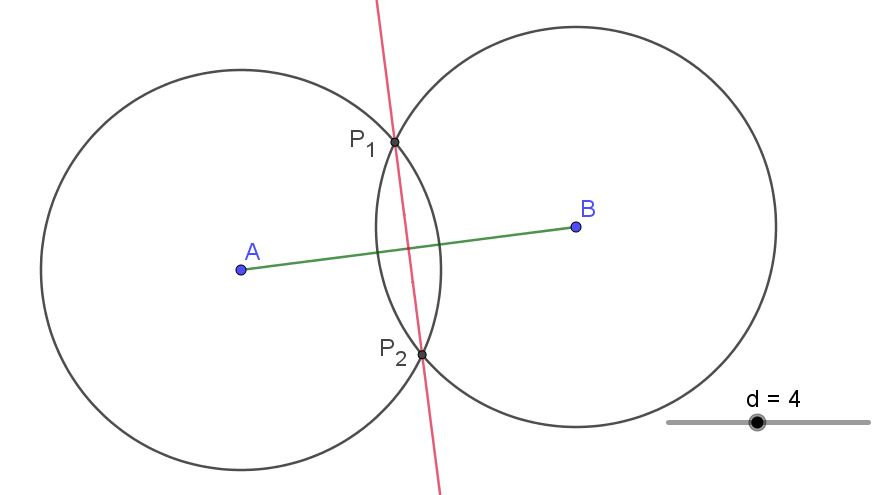
\includegraphics[width=0.98\linewidth]{figurenAuteur/mll}
\captionof{figure}{De omgekeerde eigenschap van de middelloodlijn met GeoGebra}
\label{mll}
\end{center}
\end{figure}

Beide implicaties kunnen worden bewezen met congruente driehoeken. De figuren zien er hetzelfde uit, maar het gegeven en het te bewijzen zijn anders. Je kunt met de leerlingen afspreken dat ze op hun tekening vaste kleuren gebruiken voor het gegeven en het te bewijzen. Bij de eerste implicatie steunen ze op het kenmerk zhz. Bij de tweede implicatie moeten ze beslissen wat ze, behalve het lijnstuk $[AB]$ en de gelijke afstanden $|PA|$ en $|PB|$, bijtekenen. Tekenen ze uit $P$ een loodlijn op $[AB]$, dan kunnen ze het kenmerk zz90° gebruiken om aan te tonen dat deze loodlijn door het midden van $[AB]$ gaat en dus de middelloodlijn van $[AB]$ is. Maar als ze punt $P$ verbinden met het midden van $[AB]$, dan moeten ze zzz gebruiken en hiermee bewijzen dat deze verbindingslijn loodrecht staat op $[AB]$

De eerste implicatie wordt ook ook wel als volgt geformuleerd: $|PA|=|PB|$ is een \emph{nodige voorwaarde} voor punt $P$ om op de middelloodlijn van $[AB]$ te liggen. De tweede implicatie: $|PA|=|PB|$ is een \emph{voldoende voorwaarde} voor punt $P$ om op de middelloodlijn van $[AB]$ te liggen. Even ver van de eindpunten liggen is dus een `nodige en voldoende' voorwaarde om op de middelloodlijn te liggen: 

\begin{center}
$P$ ligt op mll$[AB]$ $\Leftrightarrow$ $|PA|=|PB|$
\end{center}

Dus: de middelloodlijn van $[AB]$ is de verzameling (meetkundige plaats) van de punten van het vlak die even ver van $A$ als van $B$ liggen.

\tussentitel{Bissectrice van een hoek}

Voor de bissectrice van een hoek $\hat{A}=B\hat{A}C$ is het gedeeltelijk analoog, maar de nodige en voldoende voorwaarde is niet zomaar

\begin{center}
$P$ ligt op biss $\hat{A}$ $\Leftrightarrow$ $d(P, AB)=d(P, AC)$
\end{center}

maar wel:

\begin{center}
Voor $P$ binnen $\hat{A}$ geldt: 

$P$ ligt op biss $\hat{A}$ $\Leftrightarrow$ $d(P, AB)=d(P, AC)$
\end{center}

of: 

\begin{center}
$d(P, AB)=d(P, AC)$\\
$\Leftrightarrow P$ ligt op één van de bissectrices van de rechten $AB$ en $AC$
\end{center}

\begin{figure}[H]
\begin{center}
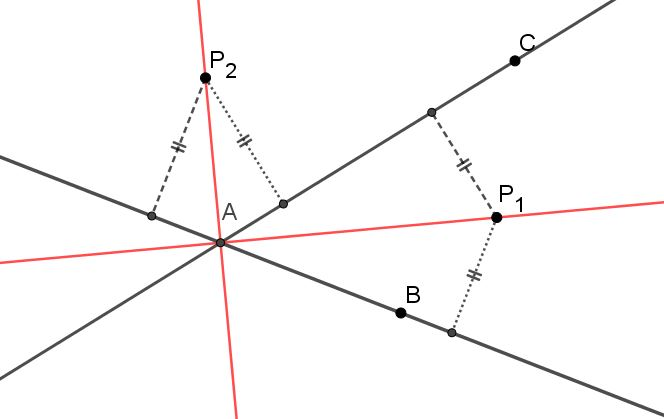
\includegraphics[width=0.8\linewidth]{figurenAuteur/biss}
\captionof{figure}{Punten even ver van twee gegeven rechten}
\label{biss}
\end{center}
\end{figure}

De meetkundige plaats van de punten op gelijke afstand tot twee snijdende rechten is immers de unie van twee rechten, die loodrecht op elkaar staan (figuur \ref{biss}).

In verband met meetkundige plaatsen van de eerste tot de derde graad verwijzen we naar de loep van UW 30/2 (Eggermont, Roelens en Vanlommel, 2014).

\tussentitel{Ruimer kader}

Schatteman (2010) pleit om de eigenschappen van de middelloodlijn en de bissectrice boeiender aan te brengen, als onderdeel van een ruimer onderzoek: welke punten liggen even ver van één punt, van twee punten, van drie punten...? Welke punten liggen even ver van één rechte, van twee rechten, van drie rechten...? Dit maakt het veel interessanter dan de aankondiging ``we hebben de definitie van de middelloodlijn gezien, nu gaan we er een eigenschap van bewijzen''.

\subsection{De gelijkbenige driehoek}

De eigenschap ``de basishoeken van een gelijkbenige driehoek zijn gelijk'' en de omgekeerde eigenschap ``als een driehoek twee gelijke hoeken heeft, dan is die driehoek gelijkbenig'' zijn erg dankbaar om leerlingen naar bewijzen te laten zoeken en te laten ervaren dat verschillende bewijzen mogelijk zijn. Je kunt de leerlingen, bv. per twee, hun eigen bewijs laten opstellen en dan alle gevonden bewijzen (in de hoop dat er verschillende zijn) samenbrengen. Het is natuurlijk niet nodig dat `alle' mogelijkheden uit de bus komen maar het zou hier jammer zijn om door teveel sturing de leerlingen allemaal op één zelfde spoor te sturen.

Om de rechtstreekse stelling te bewijzen, veronderstellen we dat de zijden $|AB|$ en $|AC|$ gelijk zijn. De leerlingen moeten aantonen dat de hoeken $\hat{B}$ en $\hat{C}$ gelijk zijn. Hiervoor hebben ze twee congruente driehoeken nodig, één met hoekpunt $B$ en één met hoekpunt $C$. Wanneer ze een rechte bijtekenen om de driehoek in twee driehoeken te verdelen, is het belangrijk dat ze erbij zeggen welke rechte ze tekenen. De tekening ziet er telkens hetzelfde uit (op de aanduiding van gelijke lengtes of hoeken na) en na het bewijs zal blijken dat dit telkens dezelfde rechte is, maar de redenering is wel telkens anders.

\begin{figure}[H]
\begin{center}
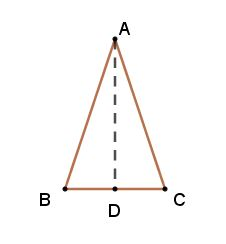
\includegraphics[width=0.4\linewidth]{figurenAuteur/gelijkbenig}
\captionof{figure}{}
\label{gelijkbenig}
\end{center}
\end{figure}

\begin{opsomming}
\item Nemen ze de zwaartelijn uit $A$, dan zijn de deeldriehoeken congruent door zzz.
\item Nemen ze de hoogtelijn uit $A$, dan zijn de deeldriehoeken congruent door zz90°.
\item Nemen ze de bissectrice van $\hat{A}$, dan zijn de deeldriehoeken congruent door zhz.
\item Ze kunnen ook steunen op de omgekeerde eigenschap van de middelloodlijn (zie 4.1): omdat $A$ even ver ligt van $B$ als van $C$, ligt $A$ op mll$[BC]$. Bij deze aanpak hebben ze de keuze tussen zzz, zz90° en zhz. 
\item Ten slotte, maar weinig leerlingen denken hieraan, is het ook mogelijk om niets bij te tekenen en te zeggen dat driehoek $ABC$ congruent is met driehoek $ACB$ (wegens zzz of zhz). Congruente driehoeken mogen immers overlappen en zelfs samenvallen...
\end{opsomming}

Voor de omgekeerde eigenschap is gegeven dat $\hat{B}=\hat{C}$ en moeten we bewijzen dat $|AB|=|AC|$. Ook hier hebben de leerlingen keuze tussen verschillende mogelijkheden. Het is hierbij belangrijk te benadrukken dat deze omgekeerde eigenschap niet zomaar een gevolg is van de rechtstreekse eigenschap. (Zie 3.1.)

\begin{opsomming}
\item Met de zwaartelijn: zzh (hm, omdat dit geen kenmerk van congruentie is, neem je beter een andere rechte...).
\item Met de hoogtelijn: hhz.
\item Met de bissectrice: hhz.
\item Ook hier is het mogelijk om te zeggen dat driehoek $ABC$ congruent is met driehoek $ACB$ (hzh of hhz).
\end{opsomming}

Nog een paar (bewijs)opgaven over basishoeken van een gelijkbenige driehoek (naar: Schmid \& Schweitzer, 1990).

\begin{opsomming}

\item In  figuur \ref{gelijkbenig1}: hoe groot is $\beta$ als $\alpha=25^\circ$ is? Voor welke waarde van $\alpha$ is de driehoek $BCD$ gelijkzijdig?

\emph{De hoek $\beta$ is het dubbel van $\alpha$. Voor $\alpha=30^\circ$ is $\beta$ dus $60^\circ$ en dan is $BCD$ gelijkzijdig omdat die twee (en dus drie) hoeken van $60^\circ$ heeft.}

\begin{figure}[H]
\begin{center}
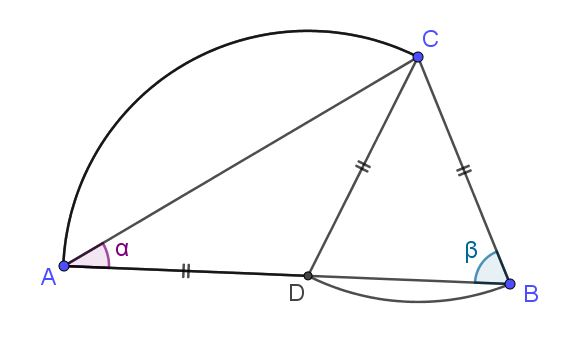
\includegraphics[width=0.75\linewidth]{figurenAuteur/gelijkbenig1}
\captionof{figure}{}
\label{gelijkbenig1}
\end{center}
\end{figure}

\item Onderzoek zonder te meten of de driehoek $PQR$ in figuur \ref{gelijkbenig2} gelijkbenig is.

\emph{Het antwoord is positief omdat de hoeken $\hat{P}$ en $\hat{Q}$ van deze driehoek gelijk zijn. We laten de lezer zelf ontdekken waarom.}
\end{opsomming}

\begin{figure}[H]
\begin{center}
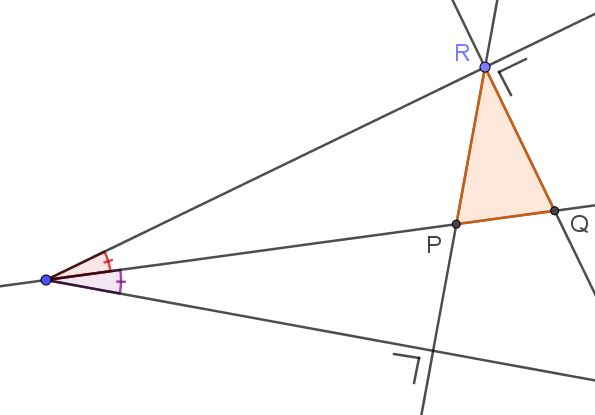
\includegraphics[width=0.8\linewidth]{figurenAuteur/gelijkbenig2}
\captionof{figure}{}
\label{gelijkbenig2}
\end{center}
\end{figure}

\subsection{Eigenschappen en kenmerken van vierhoeken}

\tussentitel{Eigenschappen en kenmerken verkennen en bewijzen}

Een mooie en eenvoudige context om eigenschappen te ontdekken, te ordenen en te bewijzen wordt gevormd door de klassieke speciale vierhoeken: trapezia, parallellogrammen, ruiten, rechthoeken, vierkanten (en eventueel ook gelijkbenige trapezia en vliegers). In De Bock \& Roelens (1990) beschreven we hoe we toekomstige leraren zelf orde laten scheppen in welke eigenschappen wel en niet gelden, om dan zelf een ordelijke theorie, met bewijzen, op te bouwen gebaseerd op de classificatie van de speciale vierhoeken. Een eigenschap die geldt voor parallellogrammen en voor ruiten, bewijzen ze best voor een parallellogram, want dan is die eigenschap automatisch ook bewezen voor een ruit. Een ruit is immers een speciaal geval van een parallellogram. Iets dergelijks in het klein kan ook met leerlingen eerste graad. Veel huidige handboeken voorzien trouwens een verkenning van wel of niet geldende eigenschappen.

De eigenschappen van het parallellogram die op die manier weerhouden worden, zijn:
\begin{opsomming}
\item In een parallellogram zijn de overstaande zijden twee aan twee even lang.
\item In een parallellogram zijn de overstaande hoeken twee aan twee even groot.
\item In een parallellogram snijden de diagonalen elkaar middendoor.
\end{opsomming}

Een voorbeeld van een eigenschap die \emph{niet} geldt: in een parallellogram zijn de diagonalen bissectrices van de hoeken. Om te zien dat de eigenschap niet geldt, tekenen de leerlingen best een redelijk `extreem' parallellogram, dat genoeg afwijkt van een ruit, want in een ruit geldt deze eigenschap wel... 

In een rechthoek gelden de eigenschappen van het parallellogram ook, want een rechthoek is een parallellogram. Er komt nog een eigenschap bij: in een rechthoek zijn de diagonalen even lang. Merk op: als ook het gelijkbenig trapezium `meedoet' in deze theorie, waarbij de rechthoek gezien wordt als een speciaal geval van een gelijkbenig trapezium, dan wordt de eigenschap over de even lange diagonalen voor het gelijkbenig trapezium bewezen en geldt die dan automatisch ook voor een rechthoek.

Al deze en andere eigenschappen zijn mooi te bewijzen met congruente driehoeken. Zoals eerder benadrukt, is het de bedoeling dat de leerlingen zelf die bewijzen leren opstellen, door geschikte congruente driehoeken te zoeken afhankelijk van het te bewijzen.

Sommige eigenschappen gelden ook omgekeerd en worden daarom \emph{kenmerken} genoemd. Dit is het geval voor de drie eerder vermelde eigenschappen van het parallellogram. 

De eigenschap ``in een parallellogram snijden de diagonalen elkaar middendoor'' en de omgekeerde eigenschap ``een vierhoek met diagonalen die elkaar middendoor snijden is een parallellogram'' kunnen worden samengevat worden door te zeggen dat het middendoor snijden van de diagonalen een \emph{kenmerk} is van parallellogrammen. Dit komt neer op de equivalentie: 

voor een vierhoek $ABCD$ waarbij de diagonalen $AC$ en $BD$ elkaar snijden in $S$ geldt:

\begin{center}
$ABCD$ is een parallellogram \\
$\Leftrightarrow |AS|=|SC|$ en $|BS|=|SD|$.
\end{center}

De eigenschap ``In een rechthoek zijn de diagonalen even lang.'' is geen kenmerk van de rechthoek. Als je immers `zomaar' twee even lange lijnstukken tekent die elkaar snijden en je verbindt de eindpunten, dan heb je een vierhoek met even lange diagonalen dat geen parallellogram hoeft te zijn (figuur \ref{tegenvoorbeeld}). Eén tegenvoorbeeld volstaat om te bewijzen dat een eigenschap niet geldt!

\begin{figure}[H]
\begin{center}
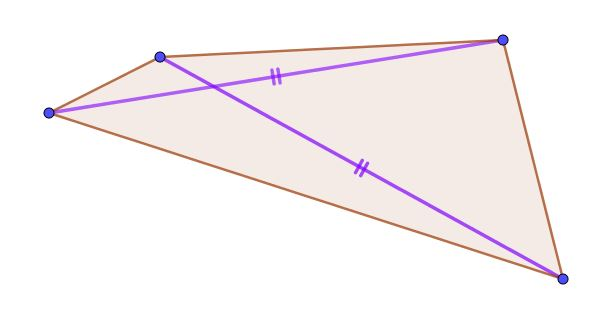
\includegraphics[width=0.85\linewidth]{figurenAuteur/tegenvoorbeeld}
\captionof{figure}{Even lange diagonalen is geen kenmerk van rechthoeken.}
\label{tegenvoorbeeld}
\end{center}
\end{figure}

Andere voorbeelden van eigenschappen die geen kenmerken zijn van het parallellogram: ``één paar overstaande zijden die even lang zijn'', of ``één paar overstaande zijden die evenwijdig zijn''. Het is gemakkelijk om telkens een tegenvoorbeeld te tekenen. Maar als je deze twee eigenschappen combineert, krijg je wel een kenmerk. Een vierhoek met één paar evenwijdige en even lange overstaande zijden, is altijd een parallellogram. Of nog: voor een vierhoek $ABCD$ geldt:
\begin{center}
$ABCD$ is een parallellogram\\ $\Leftrightarrow AB \parallel DC$ en $|AB|=|DC|$    
\end{center}


\tussentitel{Een toepassing: de schuivende ladder}

Een mooie toepassing, voor trouwe Uitwiskelaars bekend maar steeds verrassend voor de leerlingen, is de schuivende ladder. Je vraagt aan de leerlingen welke baan het middelpunt van de ladder aflegt in de ruimte als de ladder begint te schuiven. De onderkant van de ladder glijdt op de grond en de bovenkant van de ladder glijdt naar beneden langs de gevel. Het eerste idee van de leerlingen, en ook van volwassenen die het probleem nog niet kennen, is ofwel een recht lijnstuk ofwel een kromme met de holle kant naar boven gericht. De juiste baan is echter een kwartcirkel zoals in figuur \ref{ladder2},  loodrecht op gevel en grond.

De verklaring is een mooie toepassing van de eigenschappen van de diagonalen van een rechthoek. Het midden van de ladder is het midden van één van de diagonalen van een (variabele) rechthoek, zie figuur \ref{ladder3}. Omdat de diagonalen van een rechthoek elkaar middendoor snijden, is dit ook het midden van de andere diagonaal van die rechthoek. Omdat de diagonalen van een rechthoek even lang zijn, is de andere diagonaal ook even lang als de ladder en die lengte verandert niet tijdens het glijden. Dit betekent dat het midden van de ladder zich op elk moment op een vaste afstand (de halve ladderlengte) bevindt van het (vaste!) hoekpunt van de rechthoek op de grond en tegen de gevel. Dit bewijst dat het midden van de ladder op een cirkel beweegt en dus dat de baan een stuk cirkel is.\\
\begin{figure}[H]
\begin{center}
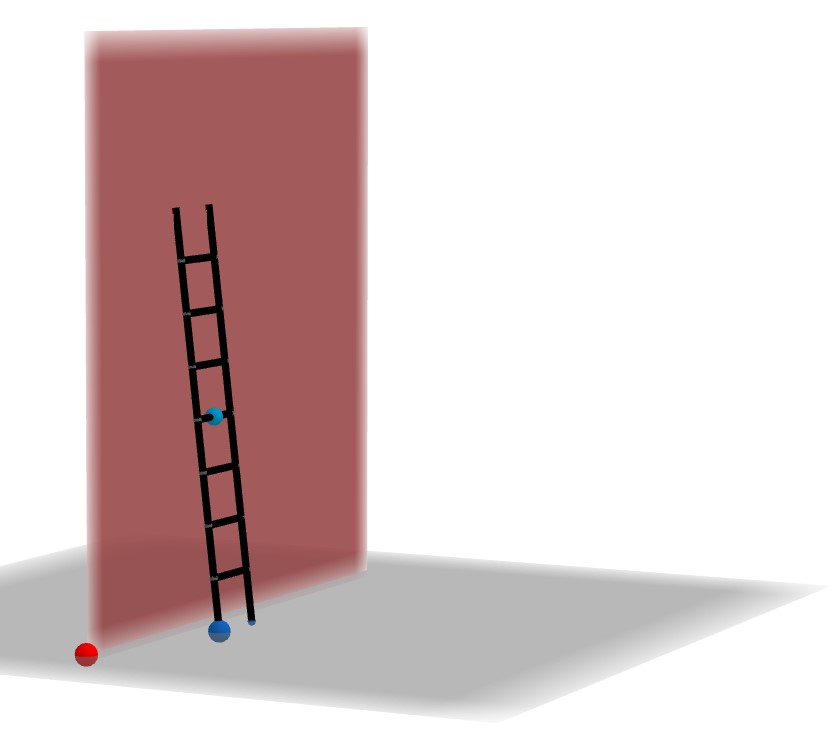
\includegraphics[width=0.95\linewidth]{figurenAuteur/ladder1}
\captionof{figure}{Het probleem van de schuivende ladder}
\label{ladder1}
\end{center}
\end{figure}


\begin{figure}[H]
\begin{center}
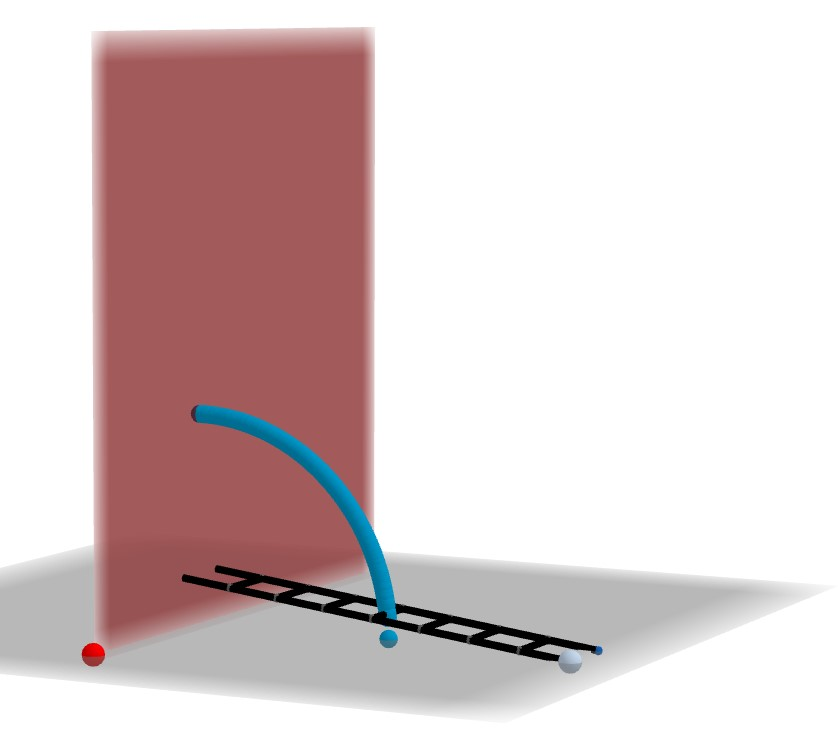
\includegraphics[width=0.95\linewidth]{figurenAuteur/ladder2}
\captionof{figure}{De baan van het middelpunt van de ladder}
\label{ladder2}
\end{center}
\end{figure}
\begin{figure}[H]
\begin{center}
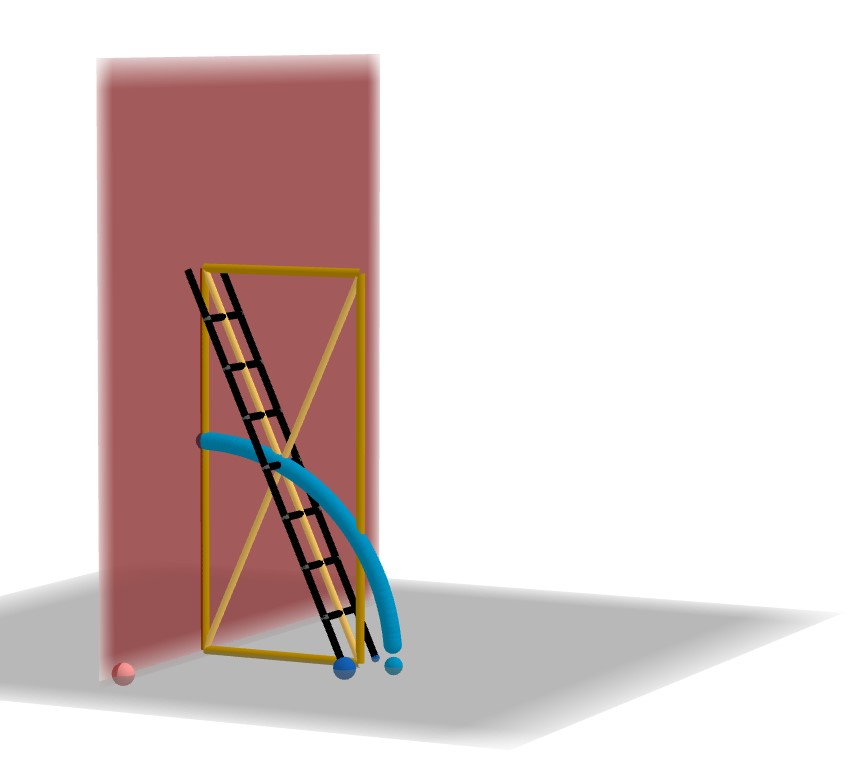
\includegraphics[width=0.95\linewidth]{figurenAuteur/ladder3}
\captionof{figure}{Bewijs met de diagonalen van een variabele rechthoek}
\label{ladder3}
\end{center}
\end{figure}

\subsection{Middenparallel en de stelling van Varignon}


\tussentitel{De eigenschap van de middenparallel}

 De eigenschap over de middenparallel zegt dat het lijnstuk dat de middens van twee zijden van een driehoek verbindt, evenwijdig is met en half zo lang als de derde zijde. Dit wordt meestal in de tweede graad behandeld, als toepassing van gelijkvormige driehoeken. Het is echter ook mogelijk om deze eigenschap te bewijzen steunend op eigenschappen en kenmerken van parallellogrammen. We vonden dit in Schatteman (2010). Op die manier zou die al in de eerste graad aan bod kunnen komen. 
 \ \\
Het bewijs met gelijkvormige driehoeken is eenvoudiger: kies je voor de eenvoud, dan stel je dit uit tot de tweede graad. Maar zoek je een toepassing van de eigenschappen en kenmerken van het parallellogram, dan is dit wel een hele mooie. We beschrijven hieronder eerst het zoekproces naar het bewijs. Dit is minstens even belangrijk als het bewijs zelf. Als je meteen het bewijs zou lezen, zou het ``uit de lucht vallen'', maar als je het zoekproces doorloopt, begrijp je waarom je het zo aanpakt. Dit zoekproces moet je natuurlijk begeleiden. 
 Je moet het niet helemaal ``voordoen'' maar zeker ook niet overlaten aan de leerlingen als zelfstandig werk...
\newpage 
\tussentitel{Bewijs met eigenschappen en kenmerken van parallellogrammen}
 
 Gegeven: een driehoek $ABC$, $M$ is het midden van $[AB]$ en $N$ het midden van $[AC]$.
 
 Te bewijzen: $MN \parallel BC$ en $2\cdot|MN|=|BC|$.
 
 Het idee is om $[MN]$ te verlengen tot het twee keer zo lang is. We construeren dus punt $P$ zodat $N$ het midden is van $[MP]$ (figuur \ref{middenparallel1}). Dan willen we proberen te bewijzen dat $[MP]$ evenwijdig is met en even lang als $[AB]$. We moeten met andere woorden bewijzen dat $BCPM$ een parallellogram is.
 
 Hoe kunnen we dat doen? Met de definitie van parallellogram of met een kenmerk. De definitie kunnen we niet gebruiken want de evenwijdigheid van $BC$ en $MP$ moeten we juist bewijzen. Het kenmerk over middendoor snijdende diagonalen lijkt hier ook niet geschikt want we weten helemaal niets over $[MC]$ en $[BP]$. Er bestaat ook nog het kenmerk over een paar even lange en evenwijdige zijden. We kunnen dit niet toepassen op de zijden $[BC]$ en $[MP]$ want dat is weer het te bewijzen. Dus: we proberen aan te tonen dat $[BM]$ en $[CP]$ evenwijdig en even lang zijn. Als dat lukt, dan is $BCPM$ een parallellogram en dan is de buit binnen!
 \begin{figure}[H]
\begin{center}
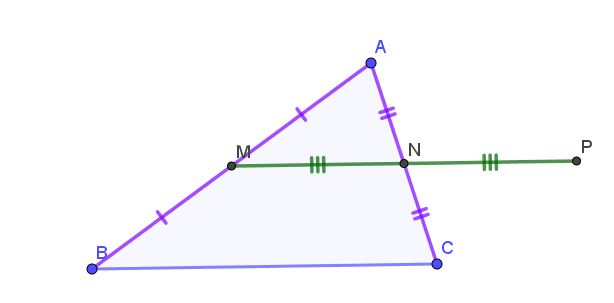
\includegraphics[width=0.9\linewidth]{figurenAuteur/middenparallel1}
\captionof{figure}{Bewijs middenparallel}
\label{middenparallel1}
\end{center}
\end{figure}
   Belangrijk is altijd de gegevens te gebruiken. We moeten iets doen met het gegeven dat $M$ het midden is van $[AB]$.
 
 $[MB]$ is even lang als $[AM]$ omdat $M$ het midden is. In plaats van te bewijzen dat $[BM]$ en $[CP]$ evenwijdig en even lang zijn, mogen we dus even goed bewijzen dat $[MA]$ en $[CP]$ evenwijdig en even lang zijn! Het volstaat dus te bewijzen dat $MAPC$ een parallellogram is (figuur \ref{middenparallel2}). Maar dat is het geval want $[MP]$ en $[AC]$ snijden elkaar middendoor!
 Na dit zoekproces ``van achter naar voor'' kunnen we samen met de leerlingen het bewijs netjes ``van voor naar achter'' opschrijven.
 
 \begin{figure}[H]
\begin{center}
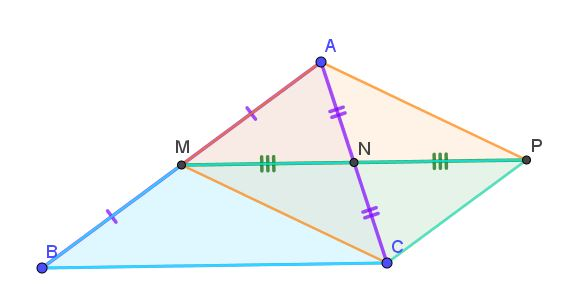
\includegraphics[width=0.9\linewidth]{figurenAuteur/middenparallel2}
\captionof{figure}{Bewijs middenparallel, vervolg}
\label{middenparallel2}
\end{center}
\end{figure}
 \emph{Bewijs}
 \begin{opsomming}
 \item Construeer punt $P$ zo dat $N$ het midden is van $[MP]$.
 
 \item In de vierhoek $MAPC$ snijden de diagonalen $[MP]$ en $[AC]$ elkaar middendoor in punt $N$ (constructie en gegeven).
 
 \item De vierhoek $MAPC$ is dus een parallellogram (kenmerk diagonalen snijden middendoor).
 
 \item Dus: $|MA|=|CP|$ en $MA\parallel CP$ (eigenschappen parallellogram).
 
 \item Dus: $|BM|=|CP|$ en $BM\parallel CP$ ($M$ is het midden van $[AB]$).
 
 \item De vierhoek $BCPM$ is dus een parallellogram (kenmerk een paar even lange en evenwijdige zijden).
 
 \item Dus: $|MP|=|BC|$ en $MP \parallel BC$ (eigenschappen parallellogram).
 
 \item Dus: $2\cdot|MN|=|BC|$ en $MN \parallel BC$.
\end{opsomming}
 
 Hiermee is het bewijs af.
 
 \tussentitel{De stelling van Varignon}
 
 Vraag aan elke leerling om een willekeurige vierhoek te tekenen en de middens van de zijden te verbinden tot een nieuwe vierhoek. Verrassende vaststelling: iedereen verkrijgt een parallellogram (dat toevallig een ruit of rechthoek kan zijn). Om dit met GeoGebra vast te stellen, is één tekening genoeg want je kunt de hoekpunten van de gegeven vierhoek nog verplaatsen.
 
 Kunnen de leerlingen het ook bewijzen? Als je deze opgave net na de middenparallel aanbiedt, geef je misschien onrechtstreeks een tip weg. Middenparallellen komen voor in driehoeken, niet in een vierhoek... Dit brengt misschien de leerlingen op het idee om de vierhoek in twee driehoeken te verdelen, met een diagonaal (figuur \ref{Varignon}). En dan gaat de rest vanzelf...
 \newpage
 \begin{figure}[H]
\begin{center}
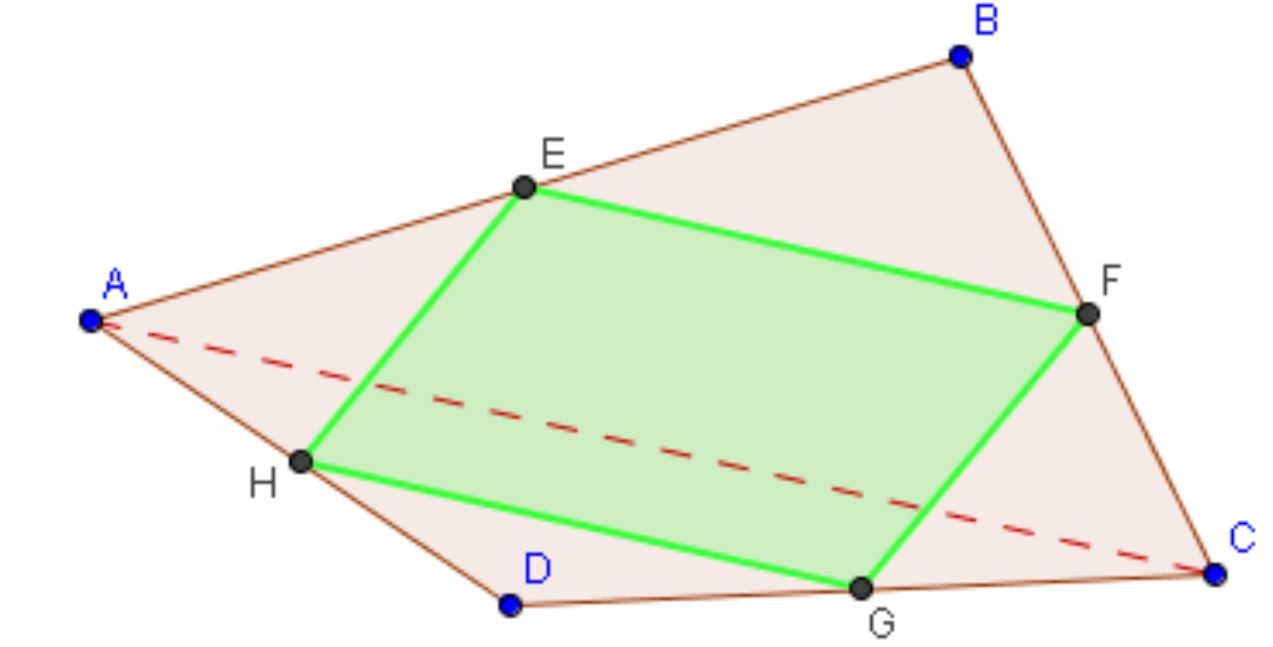
\includegraphics[width=0.9\linewidth]{figurenAuteur/Varignon}
\captionof{figure}{Bewijs van de stelling van Varignon}
\label{Varignon}
\end{center}
\end{figure} 
Het bewijs dat $EFGH$ een parallellogram is:
\begin{opsomming}
\item $EF \parallel AC$ (middenparallel in driehoek $ABC$).
\item $HG \parallel AC$ (middenparallel in driehoek $ADC$).
\item Dus: $EF \parallel HG$
\item Analoog: $EH \parallel FG$.
\end{opsomming}
Hiermee is bewezen dat $EFGH$ een parallellogram is.


Het is altijd interessant om op zoek te gaan naar speciale gevallen van een gevonden eigenschap. Ook dat is een aspect van wiskundig redeneren. Je kunt speciale gevallen nemen voor de gegeven vierhoek $ABCD$ en je afvragen wat het gevolg is voor de vierhoek $EFGH$. Het omgekeerde is nog interessanter: hoe moet je $ABCD$ nemen om ervoor te zorgen dat $EFGH$ een bepaalde speciale vorm aanneemt? 
Je kunt bv. een rechthoek verkrijgen door te starten met een vlieger of een ruit. Dat komt omdat de diagonalen dan loodrecht op elkaar staan. Maar: om een rechthoek te verkrijgen, volstaat dat de diagonalen van de oorspronkelijke vierhoek loodrecht op elkaar staan, en dat is ook bij andere vierhoeken dan vliegers het geval (figuur \ref{Varignonrechthoek}). 
\begin{figure}[H]
\begin{center}
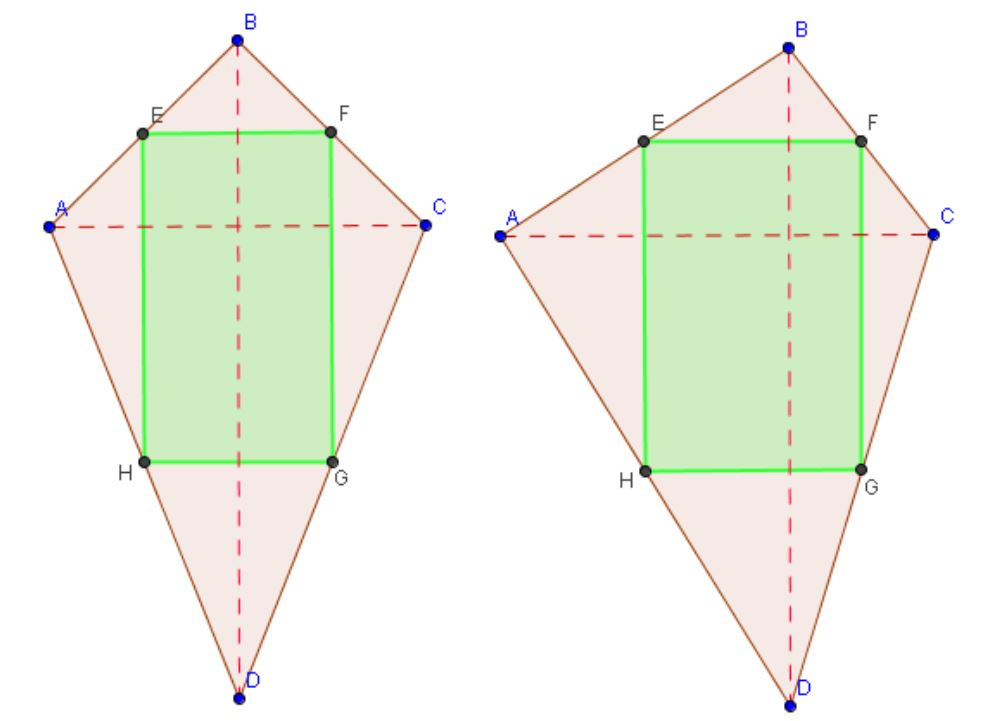
\includegraphics[width=\linewidth]{figurenAuteur/Varignonrechthoek}
\captionof{figure}{Varignon: een rechthoek verkrijgen}
\label{Varignonrechthoek}
\end{center}
\end{figure}

Wil je een ruit verkrijgen, dan moet je vertrekken van een vierhoek met even lange diagonalen. Dat is het geval bij rechthoeken en gelijkbenige trapezia, maar ook bij andere vierhoeken (zie figuur \ref{tegenvoorbeeld} in 4.3.).



\section{Bewijzen over en met oppervlakte}

\subsection{De oppervlakte van een driehoek en van een parallellogram}

De oppervlakte van driehoeken en vierhoeken vormt een mooie, toegankelijke context voor eenvoudige, visuele bewijzen. Leerlingen kunnen bv. helemaal begrijpen waarom je voor de oppervlakte van een driehoek door $2$ moet delen. In de ruimte is het fundamenteel moeilijker om te begrijpen waarom je voor het volume van een piramide door $3$ moet delen; daar gaat het in het algemeen niet door te knippen en te plakken (zie Roelens \& Willems, 2005).
Gaan we ervan uit dat de oppervlakte van een rechthoek gekend is, dan kan hieruit door te knippen en te plakken de oppervlakte van een parallellogram afgeleid worden. Beschouw een gegeven parallellogram. Door een driehoekje uit te knippen en te verplaatsen, ontstaat een rechthoek met zelfde basis en hoogte als het gegeven parallellogram, dus

$$A_{\text{parallellogram}}=\text{basis}\cdot \text{hoogte}.$$


\begin{figure}[H]
\begin{center}
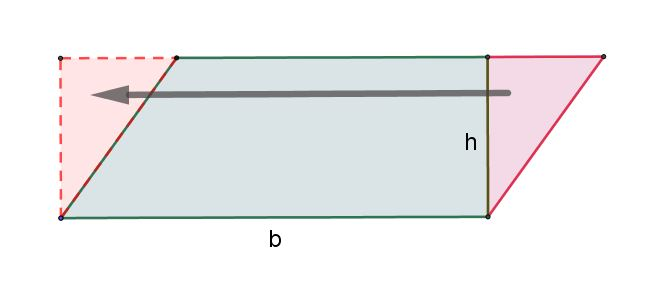
\includegraphics[width=\linewidth]{figurenAuteur/parallellogram1}
\captionof{figure}{De oppervlakte van een parallellogram}
\label{parallellogram1}
\end{center}
\end{figure}
Kritische leerlingen kunnen vragen: maar wat met een parallellogram dat `te schuin’ staat? Je kunt dan een andere zijde als basis nemen. Maar wat als je toch die basis wilt nemen? Dan maar een puzzel met meer stukjes.
\begin{figure}[H]
\begin{center}
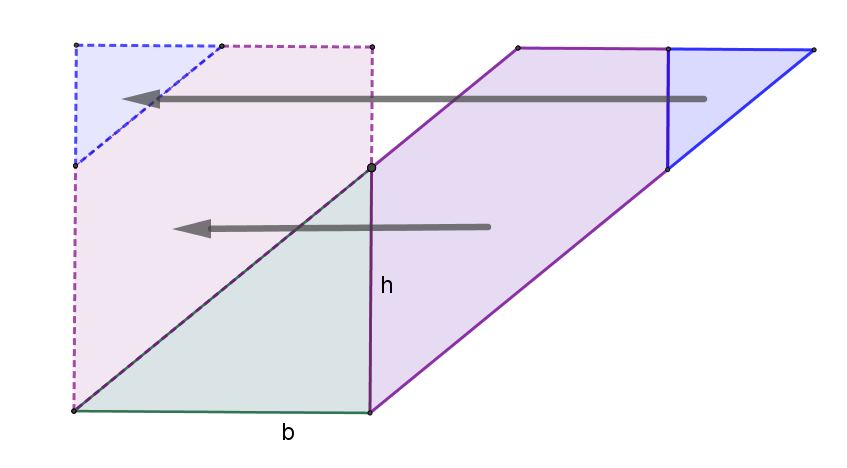
\includegraphics[width=\linewidth]{figurenAuteur/parallellogram2}
\captionof{figure}{}
\label{parallellogram2}
\end{center}
\end{figure}


Om de oppervlakte van een driehoek af te leiden van die van een parallellogram, zijn er verschillende mogelijkheden. Je kunt bv. van de gegeven driehoek en een kopie ervan, één parallellogram maken met zelfde basis en hoogte. De oppervlakte van de driehoek is de helft van die van het parallellogram, dus

$$A_{\text{driehoek}}=\frac {\text{basis}\cdot \text{hoogte}} {2}.$$

Merk op dat er hierbij veel mogelijkheden zijn (figuur \ref{mogelijkheden}). Je mag kiezen welke zijde je als basis kiest, de hoogte is dan de loodrechte afstand van het overstaande hoekpunt tot die rechte (de drager van die basis). 

\begin{figure}[H]
\begin{center}
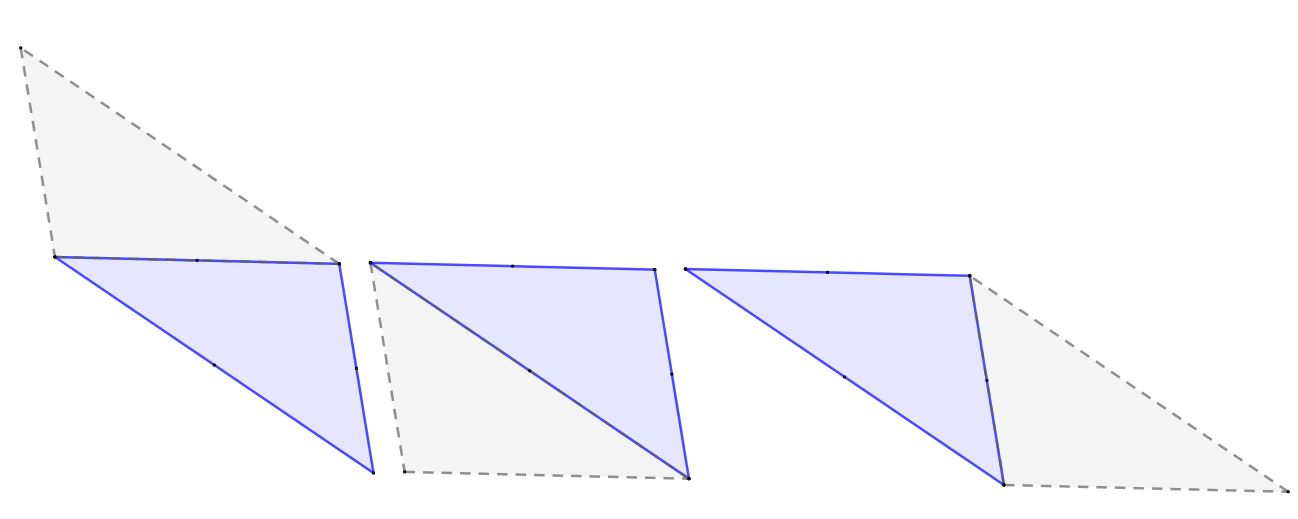
\includegraphics[width=\linewidth]{figurenAuteur/mogelijkheden}
\captionof{figure}{}
\label{mogelijkheden}
\end{center}
\end{figure}

Het `recept’ om de oppervlakte van een driehoek te berekenen, bestaat eerst en vooral uit het kiezen van een basis. De oppervlakte hangt niet af van welke basis je kiest. Dit kan heel nuttig zijn: om de hoogte uit $B$ te vinden in de driehoek $ABC$ van figuur \ref{oefke}, kun je de oppervlakte op twee manieren berekenen en gelijkstellen. 
\begin{align}
\frac{3\cdot 4}{2}&=\frac{5\cdot x}{2}\\
x&=2,4
\end{align}

In de tweede graad kunnen de leerlingen deze oefening ook oplossen met gelijkvormige driehoeken, maar ik blijf de oplossing met oppervlakten gemakkelijker vinden.

\begin{figure}[H]
\begin{center}
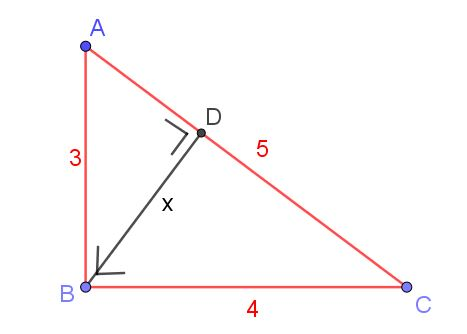
\includegraphics[width=0.6\linewidth]{figurenAuteur/oefke}
\captionof{figure}{}
\label{oefke}
\end{center}
\end{figure}

Met deze formules voor de oppervlaktes van parallellogrammen en driehoeken is meteen de volgende eigenschap bewezen: ``parallellogrammen (driehoeken) met een zelfde basis en gelijke hoogtes, hebben dezelfde oppervlakte’’ (zie figuur \ref{zelfdeopp1}).

\begin{figure}[H]
\begin{center}
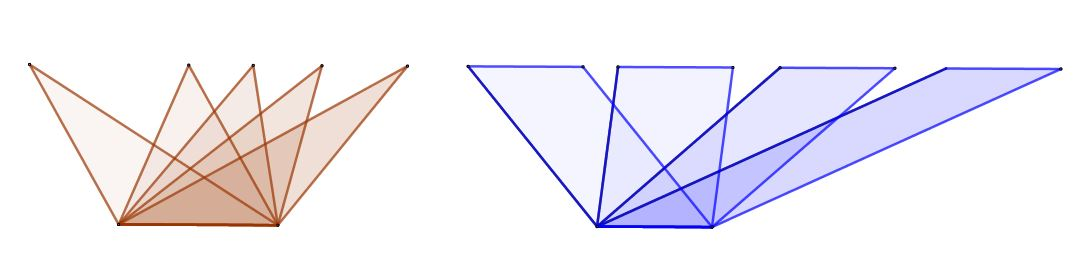
\includegraphics[width=\linewidth]{figurenAuteur/zelfdeopp1}
\captionof{figure}{Zelfde oppervlakte}
\label{zelfdeopp1}
\end{center}
\end{figure}

Dit idee is belangrijk in de Euclidische meetkunde. Als een willekeurige vierhoek gegeven is, kun je hiermee een driehoek construeren met dezelfde oppervlakte. Omdat het construeren van evenwijdigen mogelijk is met enkel passer en liniaal, is hiermee aangetoond dat het omvormen van een vierhoek tot een driehoek met dezelfde oppervlakte, mogelijk is met passer en liniaal.

\begin{figure}[H]
\begin{center}
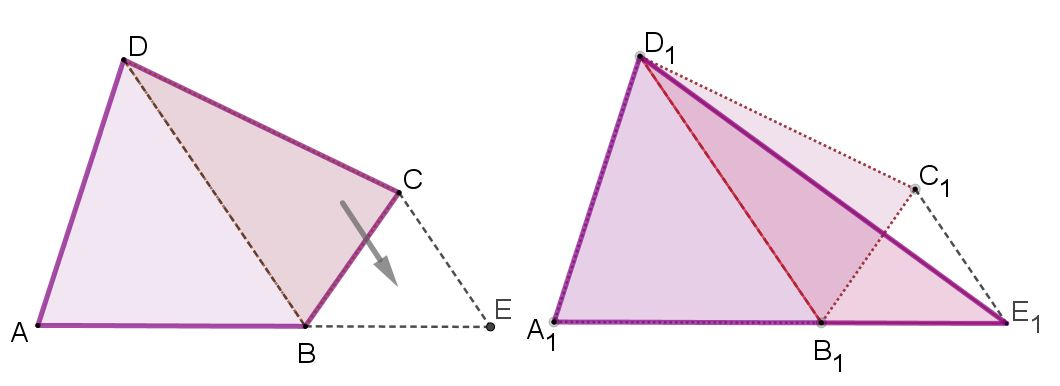
\includegraphics[width=\linewidth]{figurenAuteur/vierhoekdriehoek}
\captionof{figure}{Van een vierhoek naar een driehoek met dezelfde oppervlakte}
\label{vierhoekdriehoek}
\end{center}
\end{figure}

Met analoge knip- en plakpuzzels kan de oppervlakte van een trapezium en van een ruit afgeleid worden uit die van rechthoeken, parallellogrammen en driehoeken.

\subsection{De stelling van Viviani}

We sluiten af met een verrassend eenvoudig bewijs voor een mooie stelling.

\emph{Stelling van Vincenzo Viviani (17de eeuw)}

Gegeven: een gelijkzijdige driehoek $ABC$ en daarbinnen een willekeurig punt $P$. Bewijs dat de som van de afstanden van $P$ tot de zijden niet afhangt van $P$. Waaraan is die vaste afstandensom gelijk?

Als het waar is dat die som voor elk punt $P$ dezelfde is, dan kan die som niet anders dan gelijk te zijn aan de hoogte $h$ van de driehoek. Immers, als je $P$ in één van de hoekpunten plaatst, is die som gelijk aan $0+0+h=h$.

Het bewijs van de stelling is tegelijk creatief en eenvoudig. Verbind $P$ met de hoekpunten. Op die manier ontstaan er drie deeldriehoeken $ABP$, $BCP$ en $CAP$. Door uit te drukken dat de som van de oppervlakten van de deeldriehoeken gelijk is aan de oppervlakte van de hele driehoek, is het bewijs geleverd.

Noem $u=d(P, AB)$, $v=d(P, AC)$, $w=d(P, BC)$. De gelijke zijden $|AB|, |BC|$ en $|CA|$ noemen we $z$. Dan hebben we:
$$ \frac {zu}{2} +\frac {zv}{2} +\frac {zw}{2} =\frac {zh}{2}$$
$$u+v+w=h.$$
\begin{figure}[H]
\begin{center}
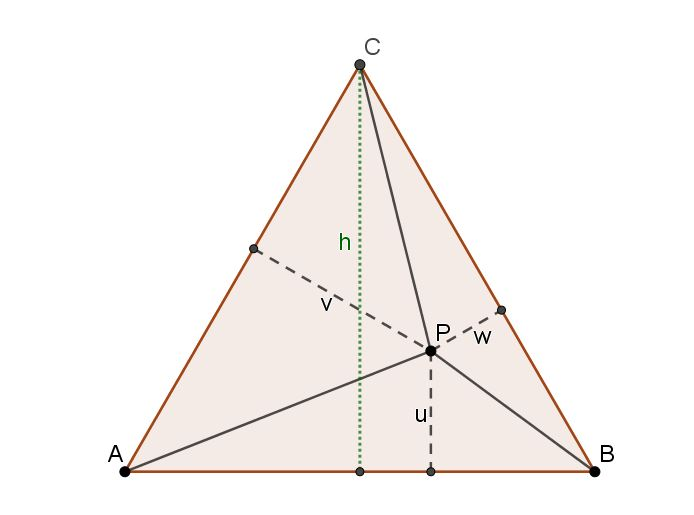
\includegraphics[width=\linewidth]{figurenAuteur/Viviani4}
\captionof{figure}{Bewijs van de stelling van Viviani}
\label{Viviani}
\end{center}
\end{figure}


\end{multicols}

\stopcontents[mainsections]			        % altijd laten staan, opsomming in inhoudstafel enkel tot loep beperken


% bronnen toevoegen
\begin{bronnen}

\item De Bock, D., Roelens, M. (1990). Vierhoeken: een verslag van een groepswerk. \emph{Uitwiskeling 6/4}, 3-7.
\item Depoorter, J., Roelens, M. Verbeeck, G. (2012). Goochelen in de wiskundeles. \emph{Uitwiskeling 28/2}, 16-58. \item de Villiers, M. (2006). Rol en functie van het bewijs in de dynamische meetkunde, \emph{Euclides 81/4} (2006), 184-188, besproken in Uitwiskeling 22/3 (2006).
\item Eggermont, H., Roelens, M. (2014). Meetkundige plaatsen. \emph{Uitwiskeling 30/2}, 15-43.
\item Eggermont, H., Roelens, M. (1995). Getallen en meetkunde in de eerste graad. \emph{Uitwiskeling 11/4}.
\item Grand’Henry – Krysinska, M. (2018). Production des premières expressions littérales dans le cadre des suites figurées. \emph{Losanges 41}, 28-47.
\item Groupe d’Enseignement Mathématique (1994). \emph{Mathématiques 2. De question en question.} Bruxelles: Didier Hatier.
\item Guissard, M.-F, Wettendorff, I. (2018a). Des figures en évolution: les carpettes carrées. \emph{Losanges 40}, 3-12.
\item Guissard, M.-F, Wettendorff, I. (2018b). Des figures en évolution: les tapis rectangulaires. \emph{Losanges 42}, 27-36.
\item Malle, G. e.a. (2008). Themanummer Begründen, \emph{Mathematik Lehren 110},  besproken in Uitwiskeling 24/1 (2008).
\item Op de Beeck, R., Roelens, M. (1998). Bewijzen, wie heeft er iets aan?, \emph{Uitwiskeling 15/1} (1998), 14-33.
\item Op de Beeck, R., Willems, J. (2010). Patronen leren herkennen in de eerste en de tweede graad. \emph{Uitwiskeling 26/1}.
\item Padilla, T. (s.d.). \emph{Divisibility trickx}. Numberphile, https://www.numberphile.com/videos/divisibility-tricks, filmpje met goocheltoer gebaseerd op deelbaarheidskenmerk.
\item Roelens, M., Willems, J. (2005). Oppervlakte en volume door de eeuwen heen. \emph{ Uitwiskeling 21/3}, 16-37.
\item Roelens, M. (2008a). Som van de hoeken van een driehoek: een interessant fout bewijs. \emph{Uitwiskeling 24/2}, 2-5.
\item Roelens, M. (2008b). \emph{Maar waarom? Bewijzen en redeneren in de onderbouw.} Plenaire lezing op de jaarvergadering van de Nvvw (november 2008).
\item Schatteman, A. (2010). \emph{Als we kiezen voor bewijzen, laten we dan niet toveren.} Kortrijk: Syllabus Dag van de Wiskunde.
\item Schmid, A, Schweizer, W. (Ed.) (1990-1991). \emph{Lambacher Schweizer Geometrie Eins/Zwei.} Stuttgart: Ernst Klett Verlag.
\item Serra, M. (1997). \emph{Discovering geometry. An inductive approach.} Emeryville, California: Key Curriculum Press.
\item van Asch, B. (2006). Bewijzen: voor alle zekerheid, \emph{Euclides 81/4}, 151-154, besproken in Uitwiskeling 22/3 (2006).
\item Van Dieren-Thomas, F. e.a. (1993). \emph{Mathématiques 1. De question en question.} Bruxelles: Didier Hatier
\item Van Leemput, G., Roelens, M. (2006). Betegelingen. \emph{Uitwiskeling 22/3}.

\end{bronnen}

